% !TEX encoding = UTF-8 Unicode
% !TEX TS-program = pdflatex

%%%%%%%%%%%%%%%%%%%%%%%%%%%%%%%%%%%%%%%%%%%%%%%%%%%%
%% TESI DI LAUREA MARTINA GHEDIN 
%% TOPIC MODA SOSTENIBILE
%%%%%%%%%%%%%%%%%%%%%%%%%%%%%%%%%%%%%%%%%%%%%%%%%%%%  Esempio con molte opzioni
\documentclass[%
    corpo=12pt,
    twoside, % impostazione per margini in libro
%   stile=classica,
    oldstyle,
    autoretitolo,
    greek,
    evenboxes,
%    tipotesi,
]{toptesi}
%%%%%%%%%%%%%%%%%%%%%%%%%%%%%%%%%%%%%%%%%%%%%%%%%%%%

\usepackage[utf8]{inputenc}   %% si può scegliere anche latin1, ma lo si sconsiglia 

\usepackage{comment}
\usepackage[T1]{fontenc}
\usepackage{lmodern}  
\usepackage{amsmath}            %% per la matematica estesa
\usepackage{lipsum}             %% Per scrivere testo fasullo in "latinorum"

%%\usepackage{natbib}
\usepackage{booktabs}           %% del Sistema Internazionale
\usepackage{latexsym}
\usepackage{caption}
\usepackage{subcaption}
\usepackage{graphicx}
\usepackage{listings}
\usepackage{color}
\usepackage{longtable}
\usepackage{wrapfig}
\usepackage{longtable}
\usepackage{setspace}
\usepackage[margin=3cm]{geometry}
                                               
\usepackage{sidecap}   %% Didascalie a fianco della figura
\usepackage[autostyle,italian=guillemets]{csquotes}   %% Per il corretto funzionamento di BibLatex
\usepackage[sorting=none,style=numeric-comp,backend=biber]{biblatex}


% Vedere la documentazione italiana o inglese di TOPtesi
% per le attenzioni che bisogna usare al fine di ottenere
% un file veramente conforme alle norme per l'archiviabilità.


% Lasciare questo per ultimo dopo aver caricato tutti gli altri pacchetti
%
% Se si è già caricato hyperref anche indirettamente (tramite altri
% pacchetti) questo statement evita di ricaricarlo
\usepackage[a-1b]{pdfx} % è utile, tienilo
\unless\ifcsname ver@hyperref.sty\endcsname\usepackage{hyperref}\fi

\hypersetup{%
	pdfpagemode={UseOutlines},
	bookmarksopen,
	pdfstartview={FitH},
	colorlinks,
	linkcolor={black}, %pink
	citecolor={black}, %pink
	urlcolor={black}
}
%%%%%%%%%%%%%%%%%%%%%%%%%%%%%%%%%%%%%%%%%%%%%%%%%%%%%%%%%%%%%%%%%%%%%%%%%

%%%%%%% Definizioni locali
\newtheorem{osservazione}{Osservazione}% Standard LaTeX
\addbibresource{bibliography.bib}

\begin{document}
\english
\onehalfspacing % Set line spacing to 1.5



\ateneo{\textsc{University of Trento}}
%\nomeateneo{Sede di Torre Elettra}
	\nomeateneo{Department of Sociology and Social Research}
	
	\titolo{Investigating customers' willingness to pay for sustainable clothing through conjoint analysis: the business case of Atotus}
	%\sottotitolo{pensare ad un sottotilo}     
	\CorsoDiLaureaIn{Data Science}

\renewcommand*\IDlabel{\\\quad Student Id: }
	
 \candidato{Martina Ghedin}[222674]

	\relatore{Prof.~Diego Giuliani}
	
	\secondorelatore{Prof. ~Giuseppe Alessandro Veltri}


	\sedutadilaurea{\textsc{Academic year} 2022-2023}
	\logosede[95 pt]{STN} %immagine del logo 
%%%%%%%%%%%%%%%%%%%%%%%%%%%%%%% Per mettere 4 relatori con classica
%\AdvisorName{Supervisors}% esempio per l'inglese
%\direttore{prof. Albert Einstein}% per il dottorato
%\coordinatore{prof. Albert Einstein}% per il dottorato
%    \relatore{prof.~Albert Einstein}% per la laurea e/o il dottorato
%    \secondorelatore{dipl.~ing.~Werner von Braun}
%    \terzorelatore{\tabular[t]{@{}l}
%    Mario Rossi\\[0.5ex]
%    Piero Negri
%    \endtabular}% per la laurea magistrale
%%%%%%%%%%%%%%%%%%%%%%%%%%%%%%% Alternativa senza opzione classica
%    \AdvisorName{Relatore}
%    \relatore{prof.~Giovanni Bianchi}
%    \secondorelatore{\tabular{@{}l}%
%    \bfseries Correlatori\\[0.5ex]
%    ing.~Lucio Verdi\\[0.5ex]
%    dott.~Mario Rossi\\[0.5ex]
%    dott.~Piero Neri
%    \endtabular}
%%%%%%%%%%%%%%%%%%%%%%%%%%%%%%% Alternativa con 4 relatori senza
%%%%%%%%%%%%%%%%%%%%%%%%%%%%%%% indicazione dei correlatori e senza
%%%%%%%%%%%%%%%%%%%%%%%%%%%%%%% opzione classica
%    \relatore{prof.~Giovanni Bianchi}
%    \secondorelatore{ing.~Lucio Verdi}
%    \terzorelatore{\tabular{@{}l}
%    dott.~Mario Rossi\\[0.5ex]
%    dott.~Piero Neri
%    \endtabular}

%%%%%%%%%%%%%%%%%%%%%%%%%%%%%%% Altro trucco per mettere il correlatore
%%%%%%%%%%%%%%%%%%%%%%%%%%%%%%% senza usare l'opzione classica
%\relatore{\tabular{@{}l@{}}
%prof.\ Albert Enstein\\[1.5ex]
%\textbf{Correlatore:}\\
%dipl.~ing.~Werner von Braun
%\endtabular}
%%%%%%%%%%
%
%%%%%%%%%% Trucco per scrivere anche un quarto relatore
%\terzorelatore{{\tabular{@{}l}dott.\ Neil Armstrong\\prof. Maria Rossi\endtabular}}

%%%%%%%%%%%%%%%%%%%%%%%%%%%%%%%%%%%%%%%%%
%%%%%%% Change the strings if you want a title page and a
%%%%%%% copyright page in another language
%%%%%%% Comment just the \iflanguage statement and the
%%%%%%% closing line of the language test if you want to
%%%%%%% make a global change instead of a conditional one.
%%%%%%% Comment the following indented lines if you don't
%%%%%%% care about the title page in English
\iflanguage{english}{%
	\retrofrontespizio{This work is subject to the Creative Commons Licence}
	\DottoratoIn{PhD Course in\space}
	\CorsoDiLaureaIn{Master degree course in\space}
	\NomeMonografia{Bachelor Degree Final Work}
	\TesiDiLaurea{Master Degree Thesis}
	\NomeDissertazione{PhD Dissertation}
	\InName{in}
	\CandidateName{Candidates}% or Candidate
	\AdvisorName{Supervisors}% or Supervisor
	\TutorName{Tutor}
	\NomeTutoreAziendale{Internship Tutor}
	\CycleName{cycle}
	\NomePrimoTomo{First volume}
	\NomeSecondoTomo{Second Volume}
	\NomeTerzoTomo{Third Volume}
	\NomeQuartoTomo{Fourth Volume}
	\logosede{STN}% or comma separated list of logos
}{}


\ifbool{classica}%
{\tomo
  \paginavuota
    \begin{dedica}
        A mia mamma

    \end{dedica}
}{%
    \frontespizio % sarebbe meglio usare l'ambiente
}

\sommario 

Slow fashion is a movement born recently to contrast the fast fashion trend. It consists in implementing a better and more sustainable supply chain with a positive environmental and social impact. Nevertheless, there is a common bias where people perceive ethical products to be too expensive. This is due partially to the actual high prices of some brands but it is also a consequence of greenwashing. In order to investigate this aspect, an empirical research has been conducted with Atotus.
It is both an e-commerce and a physical shop in Trento that sells ethical articles of clothing as a core business and it has built a circular economy network. 

A choice based conjoint analysis is performed. The first step is to build two different surveys, which have been submitted to individuals through two channels. Both questionnaires present three product profiles and individuals choose the one they would buy. Each profile is composed by one level of each attribute. These attributes are design, material and price.

Respondents are actual and potential Atotus customers reached through its social networks. Next, the collected data are given as input to the multinomial logit model to identify respondents preferences across attributes. It is the standard model, where only the individual-specific variables are taken into account. The advanced or mixed multinomial logit model includes more detailed aspects, such as heteroscedasticity and random parameters. Moreover, the willingness to pay (WTP) and the market shares of sustainable products are investigated. 

The analysis shows that all attributes are equally significant for respondents. This is the case both for the standard model and the mixed one. Moreover, the WTP shows that respondents would pay €38 more in order to buy a t-shirt made of recycled cotton and €34 for a t-shirt made of certified organic cotton. Additionally, the design, p1 and p2 are the preferred ones. As regard the shares prediction, almost 50\% of individuals would buy a product made of a  sustainable material of design p1 or p2 with a price of 50€. 

There is not much literature regarding this specific topic. Indeed, conjoint analysis is performed in many fields, but slow fashion has not been one of them. These results show a starting point of applied data analysis in this specific field. Additionally, it is possible to notice that there is a strong interest among potential and actual customers toward Atotus products and individuals' purchase behavior is coherent with Atotus pricing strategy.

%%%%%%%%%%%%%%%%%%%%%%%%%%%%%%%%%%%%%%%%%%%%%%%%%%%%%%%%%%%%%%%%%%%%%%%%%%%%%%%%%%%%

% \paginavuota 


  \tablespagetrue     %% Lista delle Tabelle
  \figurespagetrue   %% Lista delle Figure
  \indici	             %% Produce l'indice




%%%%%%%%%%%%%%%%%%%%%%%%%%%%%%%%%%%%%%%%%%%%%%%%%%%%%%%%%%%%%%%%%%%%%%%%%%%%%%%%%%%%%%%%%%%%%%%%%%%%%%%
%%% Qui Inizia il corpo dell'elaborato vero e proprio
%%%%%%%%%%%%%%%%%%%%%%%%%%%%%%%%%%%%%%%%%%%%%%%%%%%%%%%%%%%%%%%%%%%%%%%%%%%%%%%%%%%%%%%%%%%%%%%%%%%%%%%
%\mainmatter]


\part{Introduction}

\chapter{Introduction}

What has been one of the main dangers humanity has faced throughout its history? The first answers that can be given are war or climate change, but there is another great threat that has severely affected the lives of almost all human populations over time: diseases and epidemics. There were no periods - not in the past, nor nowadays - when illnesses didn't influence human lives. 

Looking at the past, the consequences of epidemics on the population were worse than today mostly because of the lack of knowledge about medical science and the poor hygienic conditions. During the bubonic plague of the 14th century, for example, 25 million deaths were reported in Europe out of a population of 100 million. The pandemic also triggered social unrest: Jews were considered responsible for the illness spread and they began to be persecuted.

\begin{figure}[]
	\centering
	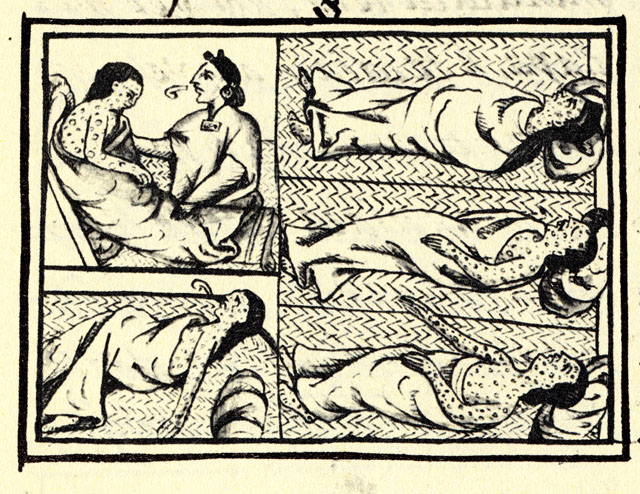
\includegraphics[width=0.4\linewidth]{0_introduction/images_introduction/FlorentineCodex_smallpox}
	\caption[Smallpox on native Americans]{Representation of smallpox disease on the Mexican population in the $XIV$ century. Figure from the Florentine Codex \cite{Sahagun1965}. }
	\label{fig:florentinecodexsmallpox}
\end{figure}

In addition, during the course of the Americas' colonization, the diseases imported by the Europeans were one of the main causes of the genocide of the local population, largely contributing to their defeat against the Spanish conquistadores. In fact, diseases like smallpox and cholera were unknown in these countries and native Americans had no antibodies to contrast them. 
Other important epidemics, famous for their consequences, were Spanish influenza, Smallpox, Typhus, HIV/AIDS, and the more recent COVID-19. 
It is straightforward to notice the effect that diseases have on our lives.

The development of modern medicine and hygiene contributed to enhancing the quality of life. An example of this is that only in the last three centuries and especially in the most economical developed countries, a significant increase in life expectancy has been observed \cite{Anderson_82}.
This increase is also happening in poorer regions, such as Sub-Saharan Africa. Although their current life expectancy is lower than that of wealthier countries, recent research \cite{Vollset_2024} predicts a significant rise over the next 30 years. This study also forecasts that this trend will lead to a global convergence in life expectancy between now and 2050.
The most plausible explanation for this future prediction is that improvements in healthcare levels lead to changes in the causes of mortality as nations' wealth increases. In poorer regions, the primary causes of death are communicable, maternal, neonatal, and nutritional diseases, whereas in more developed and wealthier countries, non-communicable diseases like cancer and cardiovascular conditions become the main causes of death \cite{CITARE_DEVO_RITROVARE_LA_FONTE}.

However, despite rising life expectancy, epidemics continue to be one of the most significant threats to populations. In fact, there was a notable increase in the frequency and magnitude of reported epidemics during the 19th and 20th centuries \cite{Anderson_82}. This makes it essential to develop effective policies to control and mitigate their impact, requiring coordinated implementation by countries within the same macro-region.
\begin{figure}[h]
	\centering
	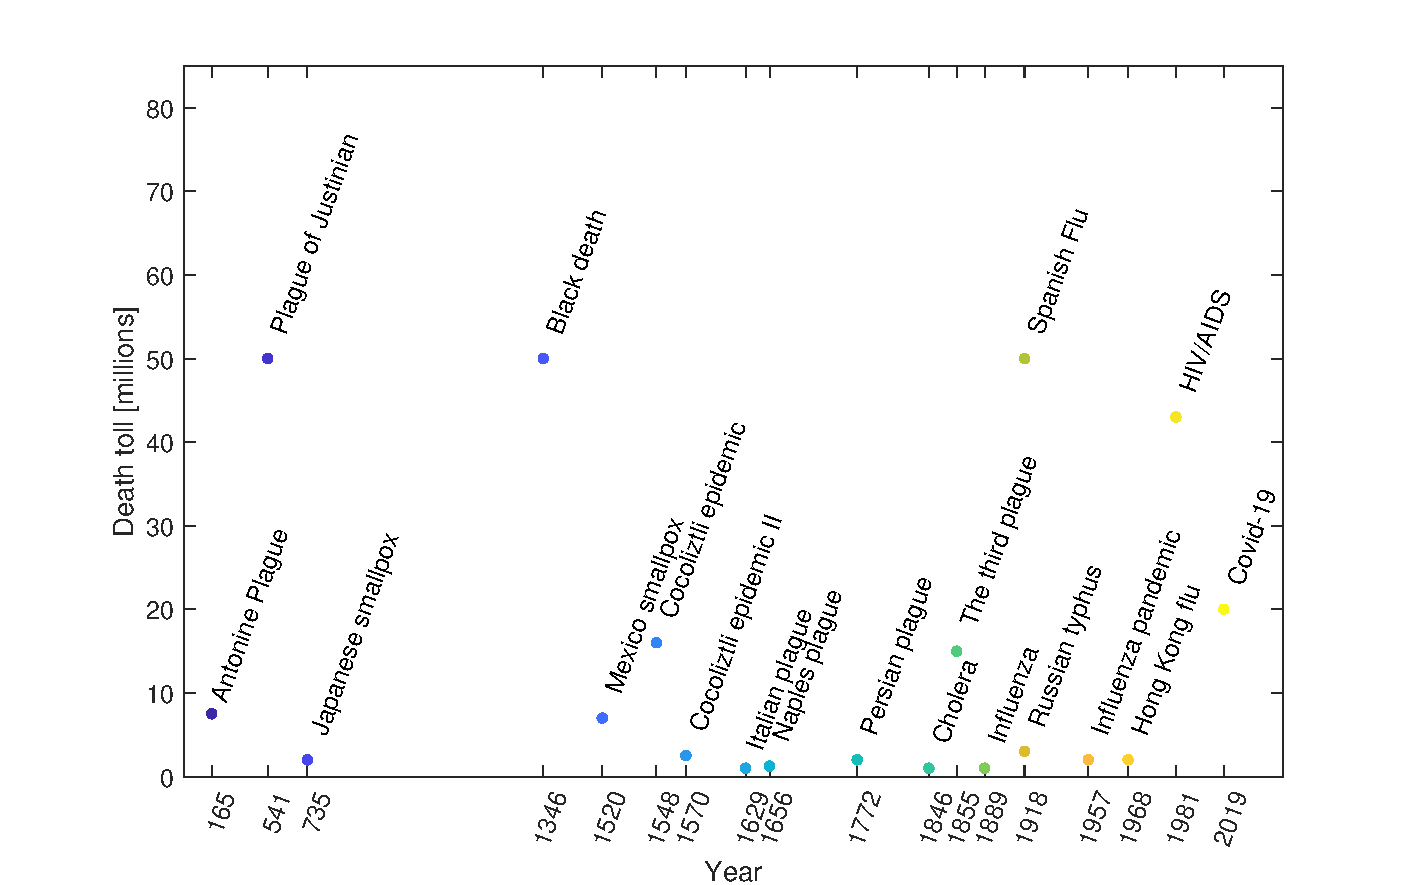
\includegraphics[width=0.85\linewidth]{0_introduction/images_introduction/worst_epidemic}
	\caption[Epidemic distribution in time]{A graphical representation of the epidemic distribution over the years and of their associated death toll. It is observable how there is an increment in the number of these event in the last three centuries. Data extracted from \cite{owid_historical_pandemics,wiki_pandemics}}
	\label{fig:worstepidemic}
\end{figure}

Figure \ref{fig:worstepidemic} highlights this trend. Although it becomes increasingly difficult to obtain reliable information about disease outbreaks the further back in time one goes, epidemics remain a tangible and present threat. This underscores the need for attention and action in shaping health policies that effectively address these dangers.
However, health status is not the only factor impacted by disease. Illness can profoundly alter relationships, work, and social life, leading to a deterioration in overall social well-being as well \cite{Yang_2020}. 
There is also an economic cost associated with the cure necessary to be healed. Only in a few nations worldwide, is treatment covered free of charge by the state. In the majority, being ill can result in having to sustain high costs, causing people to go into debt or not take care \cite{esteban_2017, Barlow2021}. 
All these effects sum together and influence how populations behave when facing an epidemic. What are the consequences of adopting a certain behavior during a disease outbreak? It's a crucial question and can help to understand how to develop more efficient policies for contrasting epidemics. It is also the question that represents the first objective of study for the present work: How can a multidisciplinary model be developed that integrates elements from both social and epidemiological aspects to provide some insights into their mutual influence during the spread of a disease?
\\
\newline
Taking a step back, it's important to understand why epidemic models are crucial and what this field of research entails.
When a new disease emerges, the primary objective is to develop a defense against it. This begins with an epidemiological investigation to understand the disease's origin, the biological mechanisms behind its spread, and its resistance to existing drugs. The goal of this investigation is to gather all available information and understand the unfolding situation.
The next crucial step involves studying the dynamics of the disease and developing a predictive model for its evolution. This process requires understanding and estimating various parameters associated with the disease, including the transmission mechanisms within the population, the reproductive rate of the infectious agent, the acquisition and persistence of immunity, and the contagion mechanism.
Creating a reliable model is not only scientifically valuable but also serves as a powerful tool for stakeholders, helping to formulate effective policies during a pandemic emergency. Theoretical epidemiology aims to provide insights and policy recommendations in this context. Furthermore, data acquisition and analysis are essential for statistically modeling epidemic coefficients. 
Ultimately, a model that can address stakeholders' questions and make predictions—whether or not safety regulations are implemented—has significant implications for society. Beyond the economic costs associated with illnesses, there are also substantial social costs. Developing tools to understand better disease transmission can help mitigate its impact and alleviate the social burden, potentially saving numerous lives.
\\ \newline
A clear example of the potential benefits of having an epidemic model is the ability to generate synthetic insights that are easy to understand and can be expressed numerically. Such models can provide answers to critical questions like:
\begin{itemize}
	\item Is the disease so infective that can cause a pandemic?
	\item What are the threshold conditions that can cause an outbreak? 
	\item What is the expected number of infections over time?
\end{itemize}

At first glance, the problem may appear straightforward. However, the creation of a model capable of evaluating every disease remains an unsolved challenge.
Research in epidemic modeling requires striking a balance between simplification and maintaining accuracy. A good model effectively reproduces key phenomena with reasonable sophistication. While creating an overly complex model that attempts to incorporate every detail of a disease might be tempting, it often requires significant effort and data. In many cases, such models don't outperform simpler ones that focus on capturing the most important dynamics of disease spread. By prioritizing essential characteristics, simpler models can provide more practical insights while remaining computationally efficient.

Over the past century, various aspects of epidemics have been extensively studied. Notable achievements by scientists include:
\begin{itemize}
	\item Development of epidemiological models using different mathematical tools, such as differential equations, networks or agent-based models \cite{Hernandez_Vargas_2022, Keeling_2005}.
	\item Predictions about the progression of epidemics or reconstructions of the events' dynamics \cite{diekmann2000mathematical, brauer2012mathematical, Ledder_2023}.
	\item Insights into epidemics, explaining phenomena like the periodicity of re-infection for certain diseases or the seasonal patterns observed in cases such as influenza \cite{Bjoernstad2016}.
	\item Understanding the effectiveness of specific strategies against outbreaks, such as vaccines or quarantines \cite{Wang_2015_review}.
\end{itemize}
Furthermore, by using multilayer networks or systems, more complex analyses can be performed. The objective is to create models capable of simulating the evolution of multiple phenomena simultaneously or to develop a more accurate representation of the real world by constructing more intricate scenarios. Examples of such models include:
\begin{itemize}
	\item The simultaneous evolution of two different diseases \cite{DeDomenico2016}.
	\item The formation of public opinions during an outbreak \cite{teslya2022}.
	\item The progression of a disease for which a vaccine exists, but where there is public fear of both the disease and potential vaccine side effects \cite{Epstein_2021}.
\end{itemize}

\section{Presentation of the work realized}
The work presented in this thesis is part of the multi-system field of research. Its focus is on understanding the mutual influence between people's behavior and an epidemic. On one hand, it examines how the presence of an epidemic affects individuals' behavior; on the other hand, it explores how these behavioral changes impact the progression and dynamics of the epidemic itself. 
For this reason a new model has been developed based on a study of existing multi-system models, and on empirical data that integrate epidemic and behavioral or opinion components.

A framework is developed where a SIR-like disease model is coupled with a new behavioral model consisting of three compartments: Heedless, Against, and Compliant individuals. These distinctions are designed to represent different courses of action taken during a disease epidemic.
"Heedless" individuals represent the segment of the population that is either unaware of the disease’s spread, particularly in its early stages, or simply indifferent to the risks. These individuals continue with their regular routines, unaware of which actions might increase their likelihood of infection.
The "Compliant" group consists of those who actively seek to avoid infection by adhering to health policies and precautions. On the other hand, the "Against" group includes skeptics who reject precautionary measures and refuse to follow established guidelines.

In the model, the main mechanism used to change behavior among different social groups is peer pressure, but also the intervention of a central global actor is considered. The fatigue from belonging to a certain behavioral spectrum (either being compliant with the rules or against them) is also considered. An epidemiological model capable of tracking both the initial phase of an epidemic and successive waves of contagion is developed, including the possibility of reinfection.

A key aspect of this work is the verification of its predictions using empirical data. For a novel multi-system model like the one implemented, it is essential to compare its results with real-world data to understand if it can accurately capture and reconstruct dynamic patterns, thereby testing its validity.

Moreover, a powerful feature of multi-system models is their ability to reveal phenomena that would not be apparent when examining the individual components in isolation. This approach allows for a more comprehensive understanding of complex interactions and dynamics. 
Additionally, understanding which of these emerging mechanisms are most relevant in real-world contexts, rather than purely theoretical models, highlights the critical need to compare the developed model with empirical data, that can help to understand better the appearing dynamics. 

Empirical data for this analysis was sourced from a research study conducted by Meta during the COVID-19 pandemic, focusing on people's opinions and behaviors.

These data were then used to investigate the model's ability to reproduce what occurred during the pandemic, specifically examining if the model could accurately simulate real behavioral patterns recorded during the emergency.

Additional aspects that were analyzed include whether peer pressure alone was sufficient to explain the observed trends in population behavior or if the influence of external global factors, such as laws implemented by governments during the pandemic, was necessary for the model to accurately reflect these trends.

%%% i risultati a lavoro finito
The main result achieved is that the model is functional and demonstrates reliability when compared with COVID-19 data. The study highlights the crucial importance of respecting quarantine measures and avoiding contact when infected, as these actions can significantly reduce the model's reproduction number, thereby limiting the spread of the disease. Altri risultati arriveranno concludendo la tesi.

\chapter{Main objectives and summary of the contents}

In this chapter, the main objectives pursued with the current work are presented and it is described the composition of the thesis. 
Starting from an analysis of the theoretical contributions already developed for epidemiology, and in particular focusing on multilayer systems and mean-field models, the following questions are studied:

\begin{itemize}
	\item how can population behaviors be effectively included in epidemiological models? What are the characteristics that must be considered?
	\item Can people's behavior influence the development of an epidemic?
	\item Is it sufficient to stop an outbreak by relying on the natural subdivision of the population into compliant and non-compliant groups regarding safety measures, or is the intervention of a central "controller" necessary to set new behavior rules?
	\item Is it useful for the model to create a quantity that express awareness of the society about the disease state? 
\end{itemize}
About the last question, consciousness or awareness is a parameter considered useful to gain insight into society's reaction to the disease. Furthermore, there can be differences in behavior when the same conditions occur at different times, such as at the beginning of an outbreak versus several months later. For this reason, it is imagined a parameter that can change its value according to such dynamic and then it is tested how effectively is in the model. 

The quantity and quality of information available to the population can make a difference in how deal with difficult situations.

Starting from these questions, the following objectives have been identified:
\begin{itemize}
	\item Create an original epidemic-behavioral multi-system model capable of tracking the development of a disease and representing behavior modification using a peer pressure mechanism within the same population.
	\item Add a second control mechanism to the model, represented by government rules that can modify people's behavior in a centralized way.
	\item Develop a comprehensive analysis of the epidemiological and behavioral model to understand its mechanisms and correctly interpret the mutual effects arising from the coupling of the social and health systems.
	\item Conduct a study using available data on population behavior during the COVID-19 pandemic to verify if the developed model can accurately reconstruct events and how people reacted to them.
\end{itemize}
The work consists of an introductory chapter \ref{ch:theo_back} where the main concepts of social science and epidemiology are presented. This chapter provides all the necessary information to understand the research. It includes a glossary \ref{subsec:glossary} of the most important terms and an overview of the mathematical tools used in epidemiology. Additionally, the different models implemented to simulate an epidemic are shown in section \ref{sec:models_categ}, with a focus on the properties of the mean fields model, which is the primary model used in the thesis. Furthermore, a historical background of the research field is provided to give a perspective on the principal milestones.
In the \ref{ch:literature_review}th chapter, a review of the literature analyzed for the thesis is presented. The articles are categorized into different main topics: epidemiology theories, opinion models, behavior models, and multi-agent and multi-system models. This subdivision highlights the most interesting aspects of each work and identifies the elements that have been considered for inclusion in the thesis.
The \ref{part:the_model} part of the thesis is composed of three main chapters. In chapter \ref{ch:model_alone}, the chosen epidemiological and behavioral models are simulated, and their characteristics are studied individually. Chapter \ref{ch:epi_behav_model} presents the model resulting from the integration of the two, which becomes a layer of a more complex multi-system model. The main features of this model are analyzed using analytical tools. The study is performed with theoretical values, sensitivity analysis, and the measurement of principal metrics, such as the reproduction rate, to provide a general description of the model and develop an understanding of it.
In chapter \ref{ch:data}, the data analysis is presented. The data available from the Meta COVID-19 research are used to test and validate the model, assessing its ability to represent a real scenario. Finally, the last chapter contains the conclusions of the thesis.
 

% ! Ci sta inizialmente concentrarsi sulle epidemie, ma  devi intrudurre anche il secondo macro filone, quello delle opinioni. é uno spin off metodologico del primo, quindi gli stumenti matematici poi sono simili, ma va detta anche questa cosa. E poi sulle opinioni hai visto quante sfumature diverse esistono sul come considerarle e anche questo è da tenere in considerazione. 
\chapter{Theoretical background}
\label{ch:theo_back}
\section{Epidemiological theory foundations}

Having a clear description of the main concepts in social science and epidemiology is essential for understanding the rest of the work. In this chapter, the theoretical basis and main concepts that will be used in the present work are defined. 

First, a brief historical review of the emergence of the epidemiology field is provided, focusing on the explanation of its genesis. Indeed, these key findings laid the foundation of modern  epidemiology. 
The following section presents a glossary of the key terms used throughout this thesis. This glossary ensures clear communication of the core concepts that will be referenced later. Initially, terms related to epidemiology are explained, followed by definitions of behavior-related concepts.

Subsequently, the most commonly used mathematical tools are introduced, including an overview of various modeling techniques. Special attention is given to the theoretical background of the mean-field model.

\subsection{Epidemiological research historical background}
\label{subsec:history}
% Se ti piace l'idea di fare un piccolo excursus storico, va bene. Le info principali sono:
% 1- primo lavoro di Bernoulli
% 2- lavori di Hamer (1906) mass action principle, epidemic description in discrete time 
% 3- Ross, formulation in continous time 
% 4- Kermack and Mc Kendrick (1927) che danno risultato bello perchè introducono "legge" del thresold di una epidemia
% Dopo aver scritto quest'ultimo evento hai il LA per parlare di come funziona un mean field model. 

The research field regarding the development of techniques to understand how epidemics can evolve during time has a history starting back in the 20th century. The first important discovery in this field must be attributed to the scientists that found the mechanism used by disease to spread. 
A first innovative work was the one did by John Snow, that during an epidemic of Cholera in London in 1854 successfully determined the source of the infection, even without knowing its etiological agent. Then advancing in the microbiological research were conducted by Pasteur and Koch. They found the etiological agent of disease, enabling the possibility to treat and prevent people from an infection. 
Then, Hamer's work in 1906 added a first major theoretical contribution. He formulated a theory about the correlation between the course of an epidemic and the interaction, or contact ratio, between susceptible and infectious individuals. It was the so called “mass -action” principle. The number of contacts between these two groups determines the spread rate of the disease. 
This law, originally written in discrete time, was then updated in 1908 by Ross, that re-written it  in continuous time. For the first time the problem could be studied using a clearly, well defined mathematical theory. Then the contributions of Kermack and McKendrick in 1927 added another fundamental principle to the modern epidemiology. They formulated a threshold theory explaining which condition can generate the development of an epidemic. The theorem affirms that a certain value -called reproduction number- must be exceed, depending on the proportion of susceptible and infectious individual. Controlling this value permits to understand if the number of infections will increase, until a peak is reached or if the epidemic is a descendent phase \cite{Mata2021, Anderson_82}. 
Their contribution with the mass action principle represents the base for the mean field model theory, that will be presented and analysed in section \ref{subsec:SIR}. 



\subsection{Epidemiological glossary}
\label{subsec:glossary}
To permit a better comprehension of the subject analyzed in the present work a list of principal concepts and terms is presented. 

\subsubsection{Micro and Macro parasite}
	The first difference when presenting infection is distinguishing the type of origin that can cause it. An etiological organism responsible for a disease can be divided into microparasite and macroparasite. The former lives and reproduces within the host, generating an immune response and the infections caused by them usually have two possible outcomes: death or immunity. Infections origins from them are shorter than the life span of an individual, and so have a transient nature.Most viral and bacterial parasite, are into the microparasitic category.
	
	Instead, macroparasite may be described by those having no direct reproduction within their host. Arthropods and helmints are in this category. They are larger and have a much longer generation times than microparasites, with a life span that can be a considerable fraction of host life span.
	
\subsubsection{Types of infectious diseases}An nnfectious disease is indicated as an illness resulting from the presence of a pathogenic microbial agent such as bacteria, viruses, parasites or other microorganism.

 It is possible to distinguish between \textit{transmittable} and \textit{communicable} disease. A transmittable disease can be transmitted between persons through unnatural routes. A communicable disease is one is one that spreads from one person or animal to another or from a surface to a person.  

\subsubsection{Disease transmission} A disease can spread in different ways: 
	\begin{itemize}
		\item Person to person: for example sexual transmission, involving direct or indirect contact.
		\item Airborne: through inhalation of infected air.
		\item Food or water borne: ingesting contaminated food or water. 
		\item Vector born: the contagion is mediated by infected animals.
	\end{itemize}
	Furthermore when the diffusion is among the same generations is called horizontal transmission, while vertical transmission is the one developing between different generations, from parents to children. 
	Zoonosis is the phenomenon in which a disease that starts in an animal species mutates and infects humans. The opposite can also happen and it is called inverse-zoonosis. 
	
\subsubsection{Epidemic disease} An increase in disease prevalence typically manifests as a rapid outbreak. This type of illness is confined to a limited geographical region, unlike a pandemic which affects a much larger area.

\subsubsection{Endemic disease} It is a disease that lasts for a long time and requires consideration of its impact on population renewal and in the number of susceptible individuals.

\subsubsection{Pandemic disease} It is an epidemic that diffuses across multiple regions, on a global scale. The severity of the disease also makes a distinction in calling a disease a pandemic. For example, a common cold is diffused in the whole world but is not defined as a pandemic by the WHO (World Health Organization). 

\subsubsection{Incubation, Symptoms, Infected and Infectious}  When a person comes into contact with an infectious individual, they may or may not become infected. The incubation period refers to the time after infection when the disease grows within the host without producing symptoms.

Symptoms refer to the physical signs of illness caused by a disease in the affected individual.

A person is described as infectious when they carry the disease and can transmit it to others, while infected refers to someone who has been exposed to the infection and has become ill.


\subsubsection{Outbreak} The rapid raise in the number of infected during an epidemic.

\subsubsection{Incidence and prevalence} The first term refers to the number of new cases within a certain period (daily or weekly for example), while prevalence is the portion of the population affected by a disease in a specific time.

\subsubsection{Immunity and herd immunity}
Immunity refers to the protection from a disease gained after contracting it. This immunity can be lifelong or diminish over time. When a person is immune, re-exposure to the virus does not result in infection, or there is only a reduced chance of being infected, known as partial immunity.

Herd immunity is a phenomenon where a large portion of the population becomes immune, either through vaccination or surviving the disease. This majority limits the spread of the illness, indirectly protecting those who are not immune by slowing or halting disease transmission.

\subsubsection{Virulence and Contagiousness}  Virulence is used to describe how aggressive, harmful, and pathogenic is a biological agent in attacking cells. Contagiousness is the capability to transmit a disease. 

\subsubsection{Overdispersion and Superspreading} Overdispersion is a term that refers to observing a larger variance than expected from a normal distribution. It is used in statistics to measure superspreading, a circumstance in which there is an anomaly (higher) number of secondary infections brought about by low numbers of spreaders.

\subsubsection{CFR, IFR and mortality excess} The case fatality rate, CFR, is the ratio between the number of deaths due to a specific disease and the total number of confirmed positive cases detected by testing. 
The infection fatality rate, IFR, is instead the percentage of people infected with the disease that are expected to die. The two quantities can have a similar value: if every person who contracts the disease and every death attributable to the disease is known and recorded, then the CFR will equal the IFR.
The excess in mortality can be calculated by observing the difference between the total death rate (due to any reason) in a month per month in a comparison between a time period with an epidemic and one without. 

\subsubsection{Reproduction number $R_0$} It is the fundamental measure of the infectiousness of a disease. It is the average number of secondary infections caused by one infected person in a fully susceptible population. If it is recalculated during the epidemic progression is called $R(t)$, a time-varying reproduction number. Finally exist also the effective reproduction number, that is obtained
rescaling the Reproduction number value with the true number of susceptible.

\subsubsection{Incubation period and serial interval} The incubation is the time after exposure in which the infection develops in the host and ends when the infected start to show symptoms. The serial interval is instead the time that exists between two transmissions in a chain of infections. 

%%%%%%%%%%%%%%%%%%%%
\section{Opinion/behaviour glossary}
To establish a framework suitable for developing and understanding behavioral models, the following key concepts from social science are outlined.
\subsubsection{Awareness} It is the knowledge that an individual has on a certain subject or situation. It changes with time and it is developed with information or experience.  
\subsubsection{Information} The term "information" is commonly understood as "knowledge communicated." However, given its crucial role in modern society, there is considerable debate about its various meanings \cite{Capurro_2003}. Today’s world is often described as an "information society," where the advancement of information technology has impacted nearly every aspect of life.

Currently, the term "information" carries two key meanings. The first, more general, definition refers to anything that is valuable in answering a question. The second definition pertains to Information Science, the discipline that manages information in all its forms. In this context, information is something with the capacity to inform. On a fundamental level, anything that is not entirely random can be considered to convey some degree of information. 

\subsubsection{Belief} It is the conviction of the truth of a statement or the reality of a being or phenomenon, especially when based on the examination of evidence, but also on matters for which there is no proof.

\subsubsection{Behaviour} It is how one acts or conducts oneself. It can depend on the response of external stimuli and have effects, especially on others.
\subsubsection{Trust} It is the sentiment of confidence associated with the ability, strength, and truth of someone or something. 

\subsubsection{Perception} It is the mechanism for which something is regarded, understood, or interpreted.

\subsubsection{Group decision-making} It is a phenomenon at the intersection of psychology, management, biology, and applied mathematics studying how people in groups interact, exchange information, and realize decisions. The decision made by the group is no longer attributable to any single individual but to the whole group. 
 
\subsubsection{Threshold theory}

It is a theory formulated by Granovetter in \cite{Granovetter_1978} regarding collective behavior. The theory posits that in a society where individuals face two possible alternatives, and their choices involve certain costs and benefits depending on how many others choose each alternative, an individual will decide based on the number of others who have already chosen a particular option when this number exceeds a certain threshold.

\subsubsection{Polarization and Consensus}

Polarization refers to the divergence of beliefs within a population. There are several mathematical methods available to measure the degree of polarization. For instance, one can collect data on opinions, beliefs, or behaviors within a group and then measure the distance between the most extreme views, or analyze their distribution across a defined range.

This contrasts with the concept of "consensus," where the exchange of opinions, information, or resources among individuals leads to widespread agreement. Both polarization and consensus can be studied and modeled using network theory.

\subsubsection{Homophily} The tendency to bond and associate with similar others. 

\section{Epidemiological models categorization}
\label{sec:models_categ}
Starting from the observation of the real world, the desire to understand better a certain phenomenon is the fundament of mathematical model development. A perfect model does not exist, because it is based on data or on assumptions that are incomplete w.r.t reality. However, a useful model guarantees the possibility of realizing general predictions and can be a powerful instrument for researchers and policymakers.  For example, an application is the estimation of certain policies' effects on the population during an epidemic: in this case, the aim is to have meaningful results, under a given set of real-world circumstances.
When working on a model the importance of the uncertainty related to claims realized with this instrument must always remembered. This concept is remarked also on the definition of mathematical model present in \cite{Ledder_2023}. 
\begin{displayquote}
	"A Mathematical model is a self-contained collection of one or more variables together with a set of rules (usually formulas and equations) that prescribe the values of those variables. Models serve as an approximate quantitative description of some actual or hypothetical real-world scenario. They are created in the hope that the behavior they predict will capture enough of the features of that scenario to be useful."
\end{displayquote}

There are several different typologies of mathematical models developed.
A first classification can be done considering the method used to obtain them: mechanistic, empirical, phenomenological or conceptual models.
The mechanistic model is based on assumptions about reality, or theoretical principles, modeled using a collection of one or more variables together with a self-contained set of rules. These models have an explanatory value on the reality they represent.
Empirical models are realized by fitting a set of data. They are a powerful instruments, because data can be modeled quite well, but they lack the explanatory value of the mechanistic models.
A phenomenological model describes the empirical relationships between phenomena in a way that aligns with fundamental theory, but it is not directly derived from first principles. These models define the relationships between variables and provide insights into the phenomenon under study. They are particularly useful in cases where no exact analytical solution exists to explain a certain scientific phenomenon.
Finally, with conceptual model, it is meant a verbal description of a real-world scenario. 

For the present work, a mechanistic/phenomenological model is the strategy used.  This is because, in the epidemiology field, the scopes that conduce to the realization of a model go beyond just fitting data. Examples of possible scopes are:
\begin{itemize}
	\item following the epidemic evolution
	\item collect and realize a structure to understand the information related to the disease 
	\item obtaining general insight about control strategies
	\item realize predictions
\end{itemize}
Considering the mechanistic category, several different types of models have been developed or are adapted to be used in epidemiology modeling. In this section, the principal typologies are now introduced. 
Regarding mean field model also a focus dedicated to its basic theretical concepts is done in section \ref{subsec:SIR}, because it represents the mathematical base model of the multi-layer system implemented in the present work. 
It is important to introduce the logic underlying its structure, its main mechanisms, and the first important conclusion that can be derived from it because it is a useful introduction to the approach that will later be employed in the rest of the thesis.

\subsection{Mean field models}
\label{subsec:mean_field}
 Mean field models, also known as compartmental models, are the first developed and most studied type of mathematical model used in epidemiology \cite{kermack1927, brauer2012mathematical, Anderson_82, anderson1991infectious}.  This model assumes that a well-mixed population is divided into several subgroups. Each compartment is a different stage of the disease under consideration. Some possible states are susceptibles, asymptomatic (infected), symptomatic (infected), infected (if in the model no distinction between symptomatic or asymptomatic is done), exposed, vaccinated, quarantined, dead, recovered, and hospitalized. The classes considered in the realized model determine its base structure. The choice to include a certain compartment depends on the disease that is modeled and on the assumptions that are under analysis. Different models can be suitable to analyze the same disease but can be used with different aims. The difference is that a more complex model can emphasize some aspects or effects of the disease, that are not highlighted by a simpler one.
 
For example, both a SIR \cite{Dehning_2020} and a SPQEIR \cite{Proverbio_2021} can be used to model COVID-19, but the second model considers explicitly quarantine, exposed and use of protections to avoid infection. Elements that cannot be observed or considered with a simpler model like a SIR.
  
In this class of models, the severity of infection is typically not considered; individuals are either infected or not. The primary focus is on describing the spread of the disease rather than its biological impact on health states. The transitions between compartments (such as Susceptible, Infected, and Recovered) are governed by differential equations.

The parameters that control these transitions are coefficients whose interpretation depends on the underlying assumptions of the model. Mathematically, these parameters determine the rate of flow between compartments.

The most critical metric in these models is the "basic reproduction number" (often denoted as $R_0$), which represents the average number of secondary infections caused by one infected individual in a fully susceptible population. It is considered a fundamental threshold in epidemiology, indicating the potential severity of an outbreak \cite{Hernandez_Vargas_2022}. 
\begin{figure}[]
	\centering
	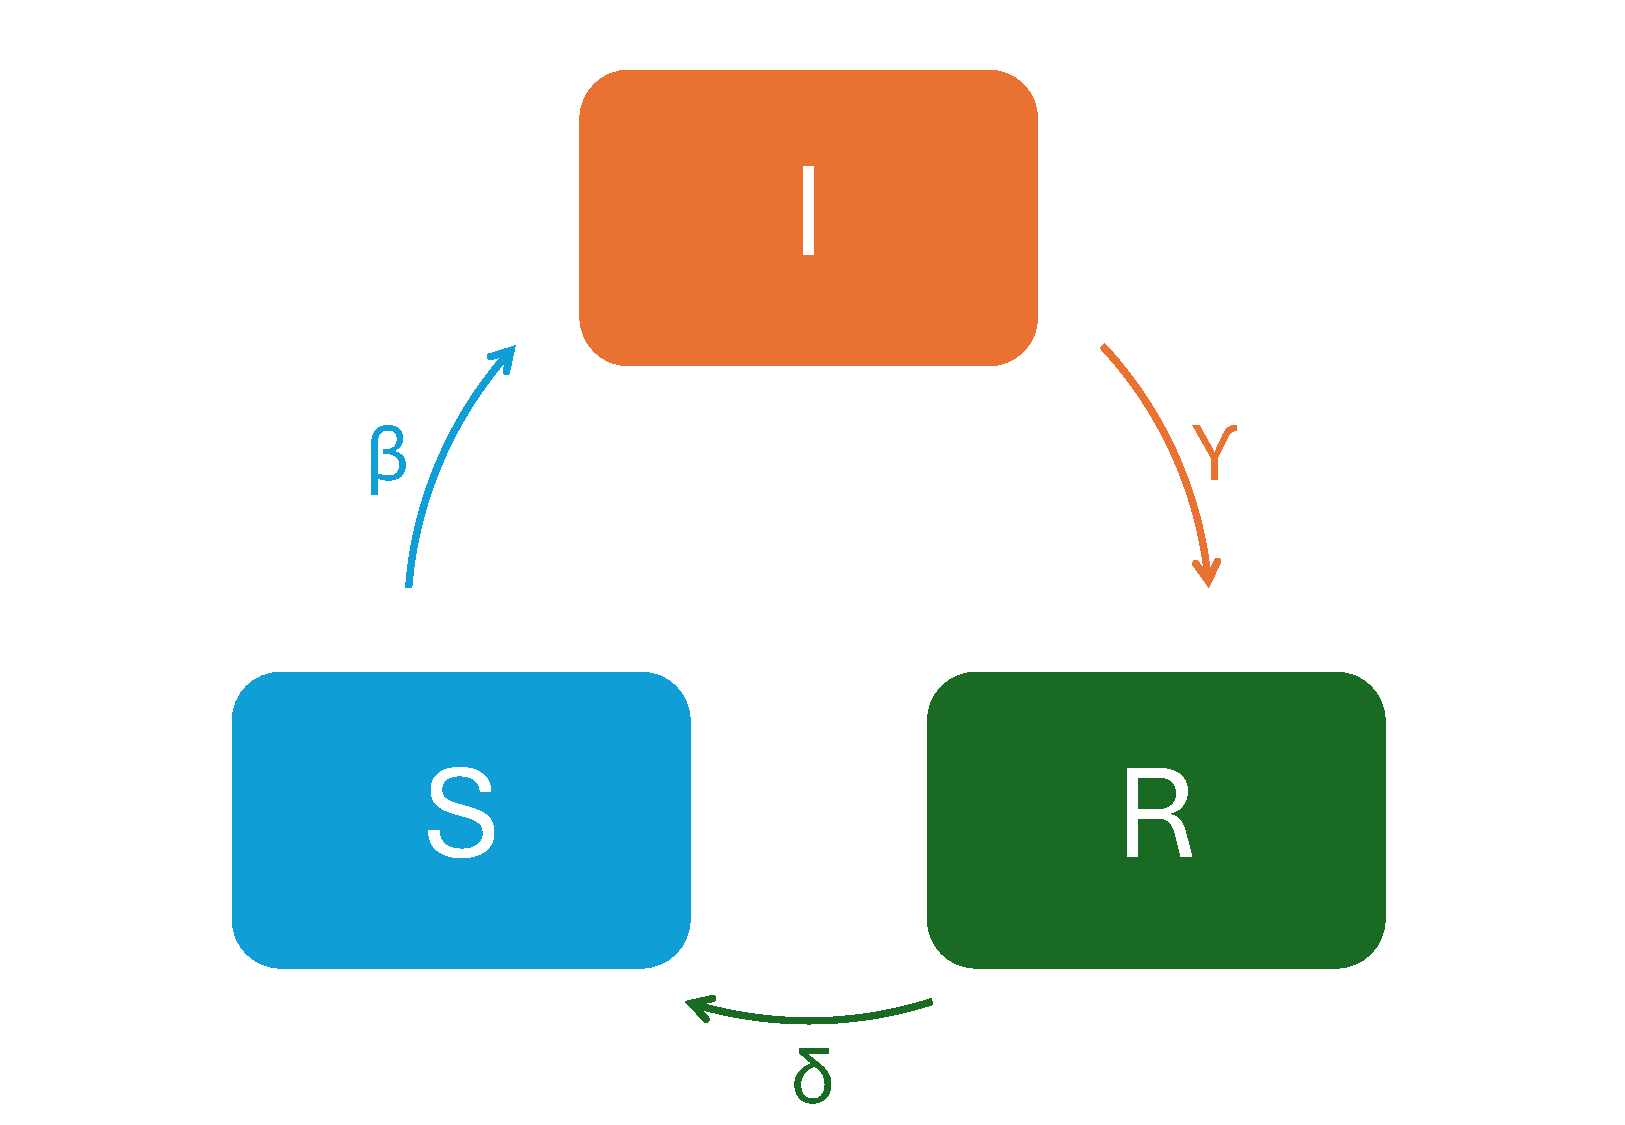
\includegraphics[width=0.65\linewidth]{0_introduction/images_introduction/SIRS_figure_compartmental}
	\caption[SIRS example]{An example of the graph structure of a mean field SIRS model. There are three compartments and the flow rate between them is ruled by the coefficients $\beta$, $\gamma$ and $\delta$.}
	\label{fig:sirsfigurecompartmental}
\end{figure}


\subsubsection{SIR model}
\label{subsec:SIR}
The foundational model for studying epidemics mathematically is the SI model. In this model, the population is divided into two compartments: Susceptible $(S)$ and Infected $(I)$. Individuals transition from being susceptible to infected, but there is no recovery, meaning once infected, individuals remain infectious indefinitely.

An extension of this is the SIR model, which adds a third compartment, Recovered $(R)$. This additional compartment represents individuals who have either gained immunity or have died, removing them from the cycle of infection. After spending a certain period in the infected state, individuals transition to the recovered state, making them no longer susceptible to the disease.

  Here the population or density of individuals is divided into three groups: Susceptible, Infectious, and Recovered. At time $t$ the three groups are identified with the symbols: $S(t)$, $I(t)$, and $R(t)$. 
The symbols used to indicate the density of each group are $s$, $i$, and $r$, while the capital letters are used to specify both the name of the groups or the absolute number of participants in each one. 

The total population size deriving from the sum of the three comportments are defined with the letter $N$.




Usually, the assumption that N remains stable is done. This is possible considering that the term epidemic identifies a disease with a duration much lower than the life of a person. Considering this assumption the number of deaths and births can be neglected. Alternatively, we can consider that the number of births, which can be modeled as an influx in the S compartment is roughly equal to the number of deaths, which is an outflux. These statements imply $s(t) + i(t) + r(t)= 1$ and $\dot{s}+ \dot{i} + \dot{r}= 0$.
The disease reproduces horizontal incidence within the population. So, it is the connection with others that causes the infection diffusion. 
$\beta$ is a coefficient that expresses the number of adequate contacts on average of a person per unit of time. The simplest way to explain the meaning of $\beta$ is to consider that not every contact between a susceptible and an infected person can generate a contagion. The formula  $\beta \frac{I}{N} = \beta i$ is then the average number of contacts with infectives per unit time of one susceptible. Finally, the number of new cases per unit of time due to the $S = N s$  susceptibles is $\beta \frac{I}{N} S = \beta N i s$. This form of horizontal incidence is called the standard
incidence. In this incidence, there is no dependence on population size \cite{Hethcote_2000}. This is because the contact of individuals daily is independent of the country dimension in which they live. 

The second transition process in the model is that individuals move from the infectious state to the recovered one at a rate $\gamma$. So the infection duration lasts an average time of $1/\gamma$ days. The $\gamma$ parameter represents the healing or recovery rate of the population. A mathematical interpretation of this term is that  
corresponds to exponentially distributed waiting times in the $I$ compartments. The transfer rate $\gamma I$ corresponds to $P(t) = e^{\gamma t}$. It is the fraction of infected that are still in their class after time $t$ of entering it and with a mean waiting time of $\frac{1}{\gamma}$.


%%
In this initial model, the immunity acquired after recovering from the illness is lifelong. It is equivalent if after being sick a person recovers or dies because it is considered that it will not transmit the infection anymore.  This assumption can be modified and there are often diseases in which after a certain period individuals become again susceptible. Another initial simplification is the one of considers the coefficient $\beta$ and $\gamma$ constant. 

Although the SIR model is quite simple it can predict a very important aspect of an epidemic, the threshold value. This effect was the main novelty studied in the pioneering work of Kermack and McKendrick \cite{kermack1927}. They found that in a fully susceptible population if and only if R0 > 1 an infection can start diffusing. Thus the origin of the term "threshold value" in epidemiology. 

The dynamic of this system has been extensively studied and analyzed during the years \cite{Breda_2012}, \cite{akinboro2014numerical}, \cite{Jard_n_Kojakhmetov_2021}, \cite{Ledder_2023}, \cite{Okabe_2020}, \cite{Prodanov_2022}, \cite{Xu_2014}, and \cite{Turkyilmazoglu_2021}. The threshold effect distinguishes between two scenarios. The first is when $R_0 <1 $. It is called "free disease equilibrium. 
In a fully susceptible population, a disease with a $R_0$ less than one does not spread. The initial small number of infected tends to zero and at equilibrium the whole population has remained in the $S$ group. This state, as proved in \cite{Hernandez_Vargas_2022}, is globally asymptotically stable. The second case is when the threshold is larger than one. Here, the number of infected grows until a peak and then decreases to zero. Both this max value of infected and the final number of susceptible can be calculated knowing the system's initial condition ($s_0$ and $i_0$) and the value of $\beta$ and $\gamma$, as explained in \cite{Hethcote_2000}. 
This second scenario analyzed with a simple SIR model permits us to immediately understand how a very aggressive infection can spread across a large part of a population. In this situation, if no countermeasures are taken in time, there can be severe consequences on the society, with social and economic damages. 

\subsubsection{Derivation of I evolution and SIR differential equations presentation}
After having theoretically presented the model, it is now explained one method to derive the mathematical form of the infection compartment evolution. 
The set of differential equations that  describe the dynamic of infection is the following:
\begin{equation}
	\begin{cases}
		dS(t) / dt = -\beta S(t) I(t)\\
		dI(t) / dt = \beta S(t) I(t) - \gamma I(t)\\
		dR(t) / dt =  \gamma I(t)
	\end{cases}
\end{equation}
Here $X(t)$ is indicated as the population at time $t$ in the X compartment. Remember that the assumption of constant population size is also done, so $S(t)+I(t)+R(t) = N$ holds.

The number of infected, with an interval  $\Delta t$, that in a base case can coincide with one day, is given by the equation:
\begin{equation}
	I(t+\Delta t) = I(t) + [\beta S(t)I(t)/N - \gamma I(t)]\Delta t
\end{equation}

If the value of N is large, the variables can be considered as continuous, and imposing a time interval close to zero it becomes:

\begin{equation}
	\frac{d I(t)}{dt} = \lim_{\Delta t \rightarrow  0} \frac{I(t+\Delta t)-I(t)}{\Delta t} = \beta S(t) I(t)- \gamma I(t)
\end{equation}

Consider now the initial state of the system. At the beginning of the disease, considering that there are few infected, the majority of the population is in the susceptible groups, so $S(0) \approx N$. Furthermore, during the initial days of contagion diffusion, this quantity remains stable. Considering this approximation, we have 
\begin{equation}
	\frac{d I(t)}{dt} = (\beta S(0)-\gamma)I(t),
\end{equation} 
which gives now a differential equation with only a variable, $I(t)$, that has a well-known solution:

\begin{equation}
	I(t) = I(0) \exp ^{(\beta S(0)- \gamma)t}
	\label{eqn:sol_I}
\end{equation}



From the analytic solution of the infectious dynamic equation in \ref{eqn:sol_I}, we can see what happens at the beginning of an epidemic.  If the exponential argument has a positive sign it is observed an exponential increase in the number of infected. While, in the opposite case, infected people tend to zero. 
The value $\frac{ \beta}{\gamma} S(0) = 1$ is defined as the epidemic threshold. In the initial phase of the epidemic the relation $\frac{ \beta}{\gamma} S(0) = \frac{ \beta}{\gamma} N $  holds. 
This quantity, normalized, is called the basic reproductive rate, and indicated with the symbol $R_0$.

It measures the intensity of the contagion or the number of secondary infections a sick person can generate. Analysing the equation of susceptibles, with this model we see that it is always decreasing. In the SIR model, if the condition to start the epidemic is satisfied after an increase in the number of Infected, there is a point at which $\frac { \beta}{\gamma} S(0)$ becomes less than one. It is when this happens that the peak of the $I(t)$ curve is reached. Then, the disease begins its falling phase. It is the natural behavior of an epidemic.

\begin{figure}[h]
	\centering
	\subfloat[][\emph{}]
	{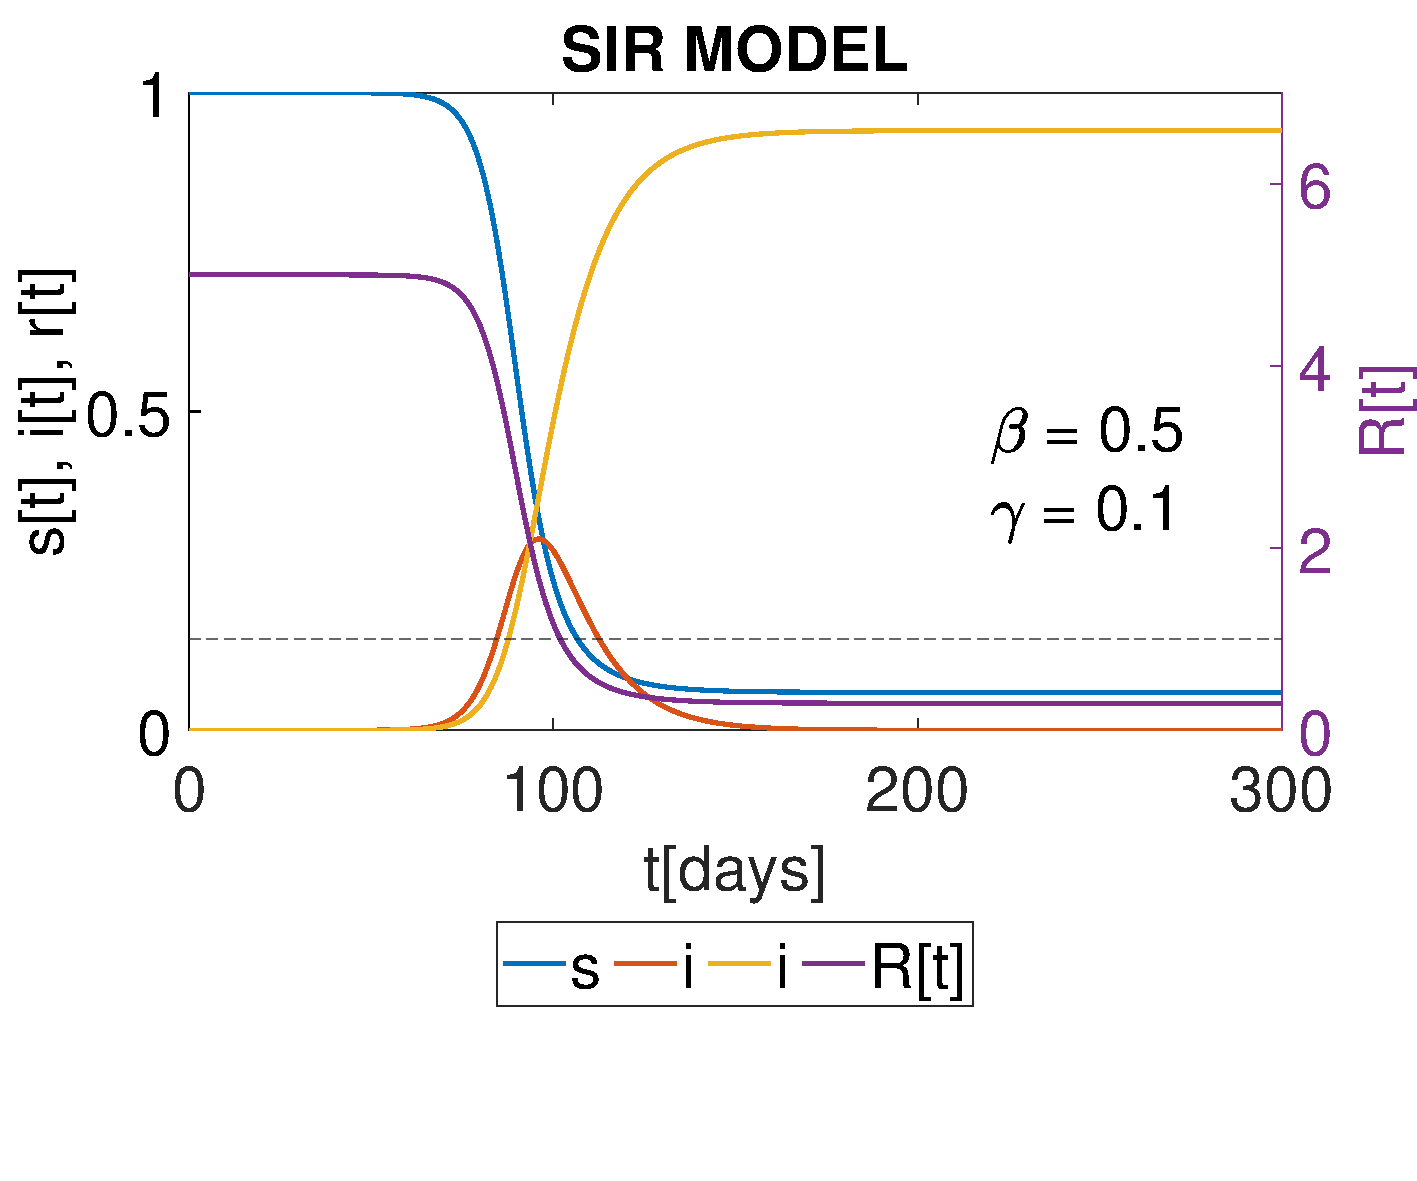
\includegraphics[width=0.48\linewidth]{0_introduction/images_introduction/sir_con_rt}} \quad
	\subfloat[][\emph{}]
	{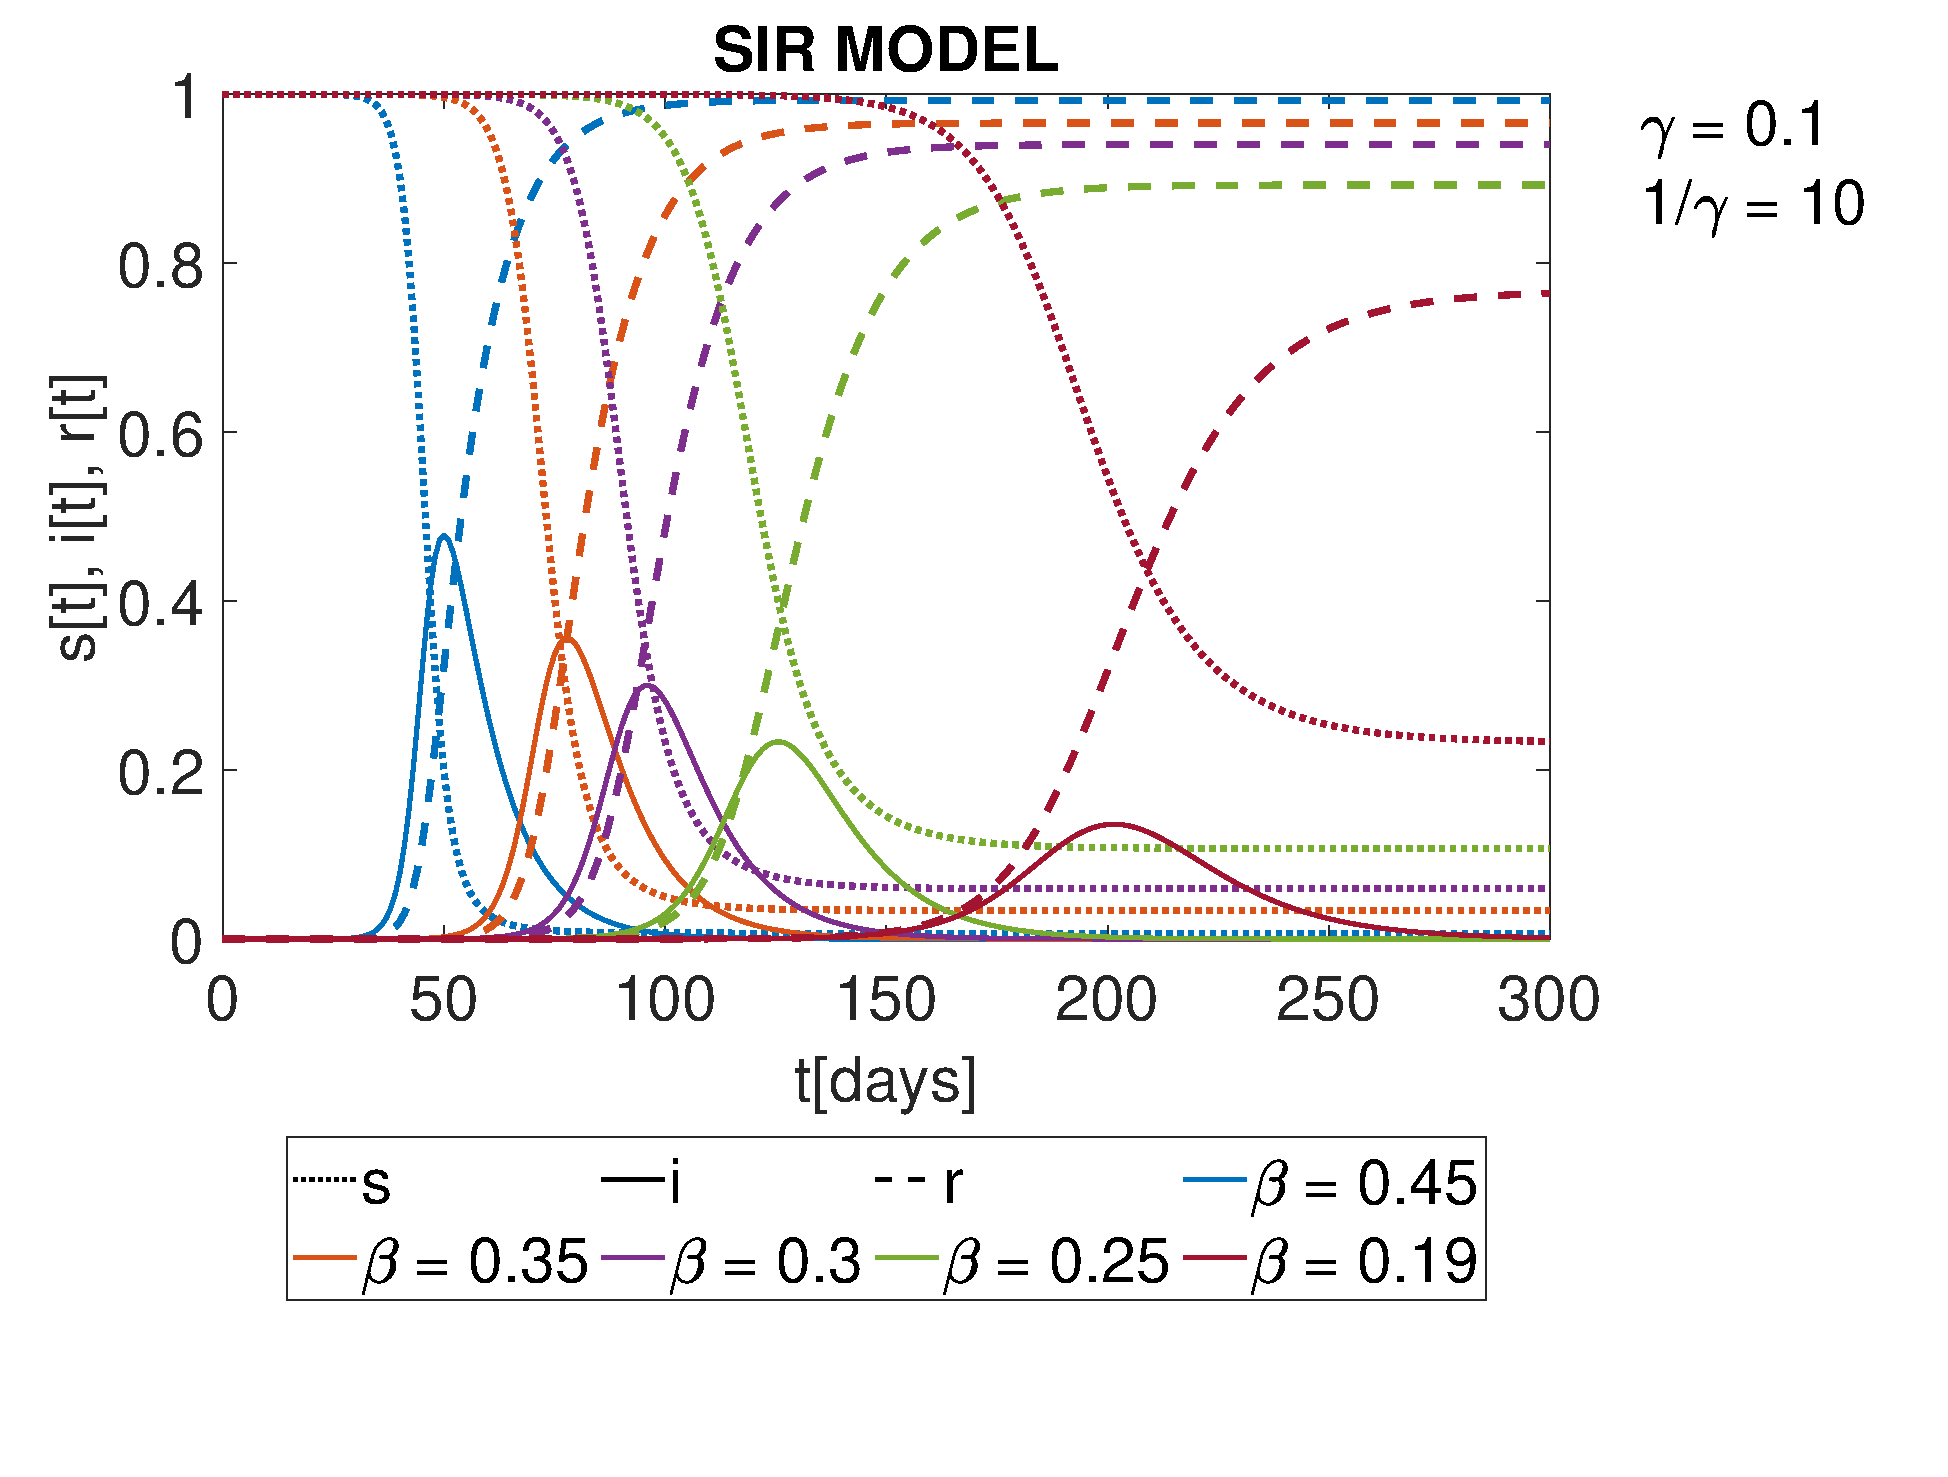
\includegraphics[width=0.48\linewidth]{0_introduction/images_introduction/sir_multipli_beta}} \\
	\caption[SIR dynamic example]{SIR system numerical solutions. Figure a) shows the evolution of compartments in the case of an epidemic. The violet dotted line represents the time-dependent $R_0(t)$. It can be seen that when this parameter is equal to $1$, the number of infected reaches its maximum value. In b) are presented different evolutions of the disease varying only the $\beta$ coefficient. The smaller its value the flattened and the more delayed the infectious curve is.}
	\label{fig:sir_example}
\end{figure}
Other two interesting quantities to consider when a new disease appears are the rate of increase of the infectious and the final size of remaining susceptible at the end of the epidemic. There is a large difference when a population suffers from an epidemic if this ends rapidly because a lot of people get sick or if this number can be controlled, and the infectious curve is flatter. A strategy to flatten the curve can reduce the contact between susceptibles, actuating social distancing or avoiding contact with infected, implementing quarantine measures. These are two simple examples of actions that reduce the value of $\beta$. Another countermeasure is represented by vaccination. Its immediate effect on the epidemic is to remove susceptibles people, so the disease can afflict only a small group and be quickly extinguished. 

\subsubsection{Stochastic models} 	
This is a group of models deriving by the mean-field, but using a different mathematical approach.
In this typology, the transition from one state to another is determined using a function of probability.  Conceptually are derived using the same framework used with ODE models. They are useful when the disease to study has a lower number of infected or if there is a connection between the epidemic outcome and changes in individual dynamics. This is called demographic variability, and it concerns changes in transmission, births, recovery, or deaths within the population. Using stochastic models with Monte Carlo simulations can be useful to investigate epidemic models on networks \cite{Allen2017}. 
The two most important types of models using this approach consider the time variable as continuous, $t \in [0, \infty) $and then the state variable is either discrete (Continuous-Time Markov-Chain) or continuous (Stochastic Differential Equations).
Referring to the SIR model to make a simple example here the S and I compartments are modeled as random variables. The probability of individuals changing groups depends on infection and recovery, the possible events that can occur. It is called transition probability. 
In a Markov chain approach the transition probability is discretized, and there is no dependence on the history of the epidemic to know how it will evolve at time $t + \Delta t$. It is necessary to know only the current state of the process at time $t$. 
In the Stochastic differential equation, the random variables are continuous. 

\subsection{Networked models}
\cite{Newman2002}, \cite{VanMieghem2009}, 
The evolution of a disease is considered over complex and realistic networks. The focus of this type of model is to understand how the network structure influences the epidemic by observing parameters such as the rate of spread.

In this framework, the nodes of the graph represent individuals (with all the properties that the modeler deems relevant for the study), while the edges represent interactions between people. Nodes can also represent subgroups of people, and using weights on edges makes it possible to characterize the strength of these interactions.

Only if this class of model is highly capable of realistically reconstructing a real network can it be a reliable instrument, and achieving this requires very complex work.
\subsection{Agent-based models}

VEDI E AGGIUNGI ANCHE \cite{Tizzoni2014}

DA WIKI INTEGRA: "An agent-based model (ABM) is a computational model for simulating the actions and interactions of autonomous agents (both individual or collective entities such as organizations or groups) in order to understand the behavior of a system and what governs its outcomes."

Agent-based models are an alternative technique used to represent disease evolution. This approach is implemented based on the observation of spontaneous connections made by individuals. 
An advantage of this type of model is that it offers a very intuitive approach to epidemic modeling. Using an individual perspective guarantees an immediate interpretation of the model. A precise agent-based model can provide a greater understanding of the illness under consideration and direct information about countermeasures to implement to stop or mitigate its spread. However, to be powerful and capable of performing good analyses and predictions, a lot of information must be integrated into the model. 
\begin{figure}
	\centering
	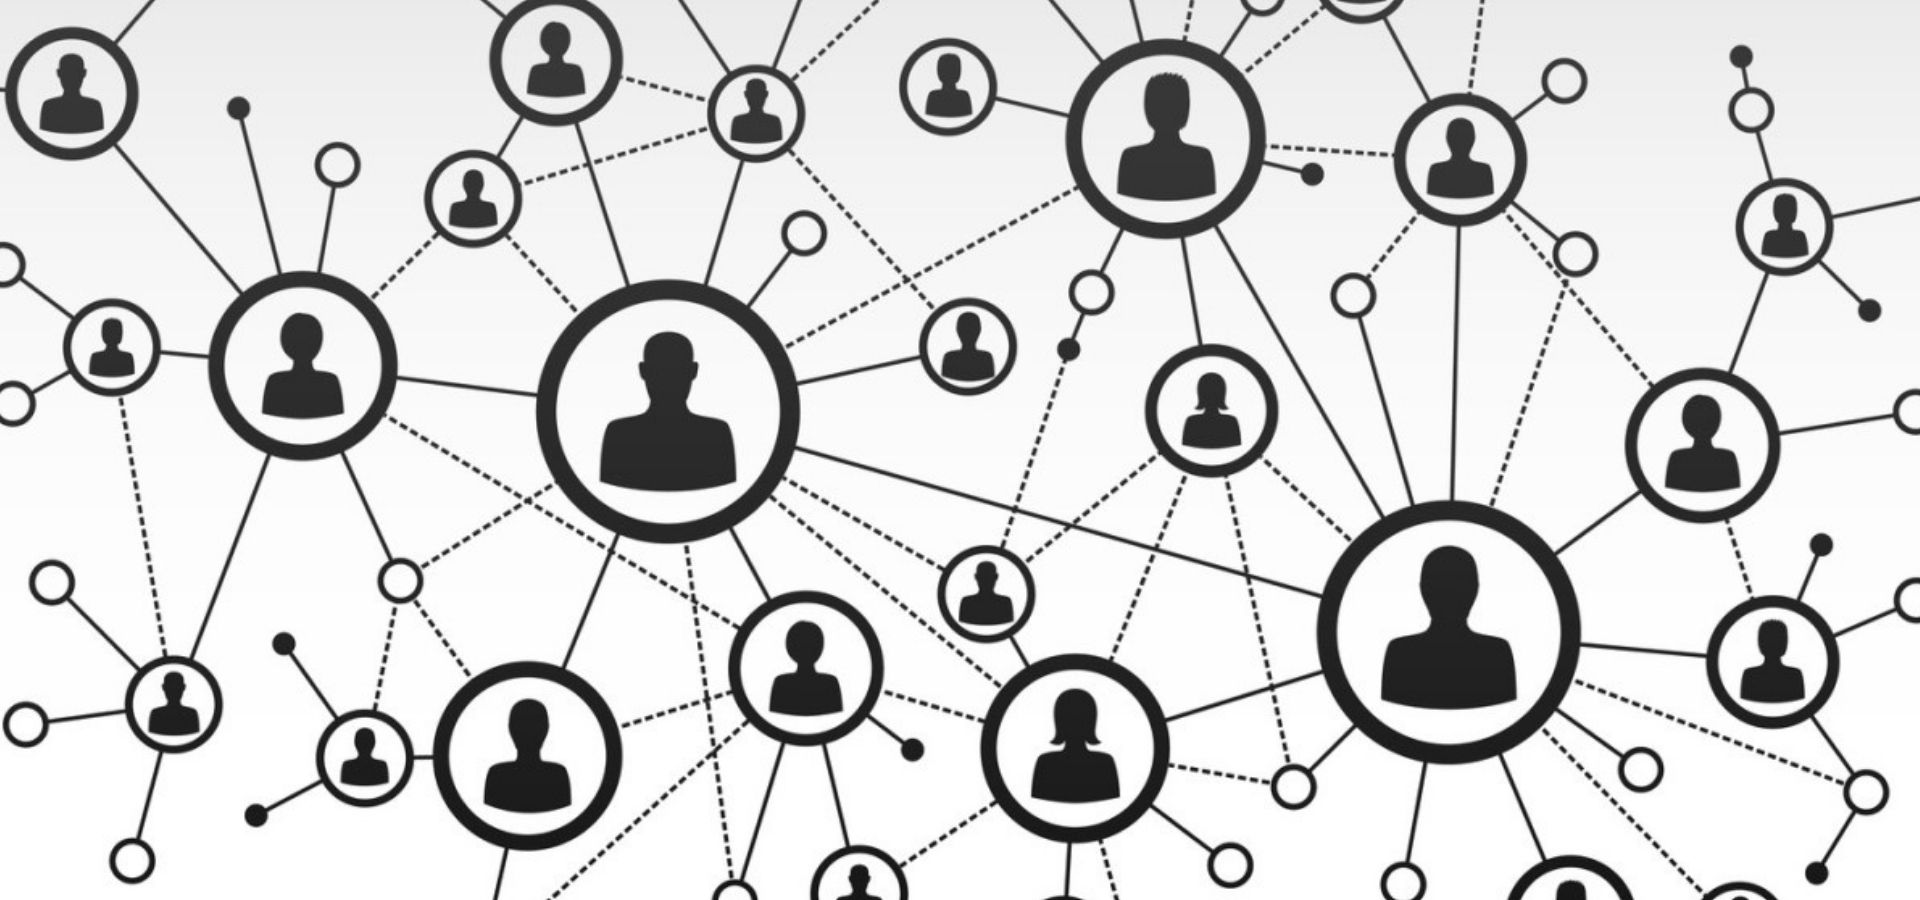
\includegraphics[width=0.5\linewidth]{0_introduction/images_introduction/agent_based}
	\caption[Agent based network representation]{Agent based network representation}
	\label{fig:agentbased}
\end{figure}

%%

An example of a possible mathematical implementation of this class of models is now briefly presented. One possible technique to describe peer-to-peer contact in a graph structure is realized through a probabilistic framework. Here, assuming a total of $n$ agents in the model, spread processes can be described as a function of probability. Using Markov processes, each agent has a certain probability of transitioning from one state of the disease to another. To calculate the value of these probabilities, both the information derived from the network structure and parameters related to the disease, such as infectivity and recovery rates, are used. In this way, a stochastic evolution model of the processes is developed.

Considering an SIS model described with a Markov process: it has a dimension of $2^n$, while implementing an SIRS model requires a dimension of $3^n$. Because the size of models developed in this manner becomes rapidly enormous, a mean-field approximation is employed. It is based on the assumptions of a network composed of a sufficiently large number of agents and on the independence of these nodes. With this technique, by taking expectations, the transition rates of individuals are approximated. Using these approximations, the boundary values of the agent's probability of infection can be determined at each time step \cite{Hernandez_Vargas_2022}.

\subsection{Multilayer systems and networks} 

AGGIUNGI ANCHE \cite{Wang_2019} \cite{Krickel_2023}

The complex dynamic of interactions existing in the real world, develops in multiple patterns, with complicated relationships. This connection can change over time, and using the theory of multilayer systems it can improve the comprehension of such complexity. Additional information can be added to the model, for example, different types of interactions, like physical contact or information sharing, time dependency coefficients, or reliance between different parameters in nature, creating cause-effect relationships. 
It is a more recent development of the research, the traditional network theory was revisited, to create a framework that can include multiple networks, that evolve and influence each other \cite{DeDomenico2016} and can be helpful to manipulate complex systems like human relationships. Some interesting results obtained are the possibility that the onset of one disease can depend on the onset of the other one. There can be regimes in which the criticality of the two dynamics is interdependent and others in which the critical effect is only one-directional \cite{DeDomenico2016}. 
One possible way to develop models with this structure is to imagine that each layer represents a different type of interaction. An epidemiological example is a layer in which the physical contact between people is simulated and another represents social structure, the network of relations that every person has. This instrument provides a natural representation of coupled structure and dynamical processes. It has been presented in multiple works in the past years, for example in CITA. 
The dynamic realized in multiple systems can be single or coupled. In the first, there is a top layer with its dynamic evolution running on top of a multilayer network. The coupled structure instead is the one in which the phenomena described in each layer evolve with the influence of what is happening in the other. 
Multilayer networks have multiple dimensions of connectivity, called "aspects" and they have to be considered simultaneously. 
They can also be considered with two different mathematical structures. 
\begin{figure}[]
	\centering
	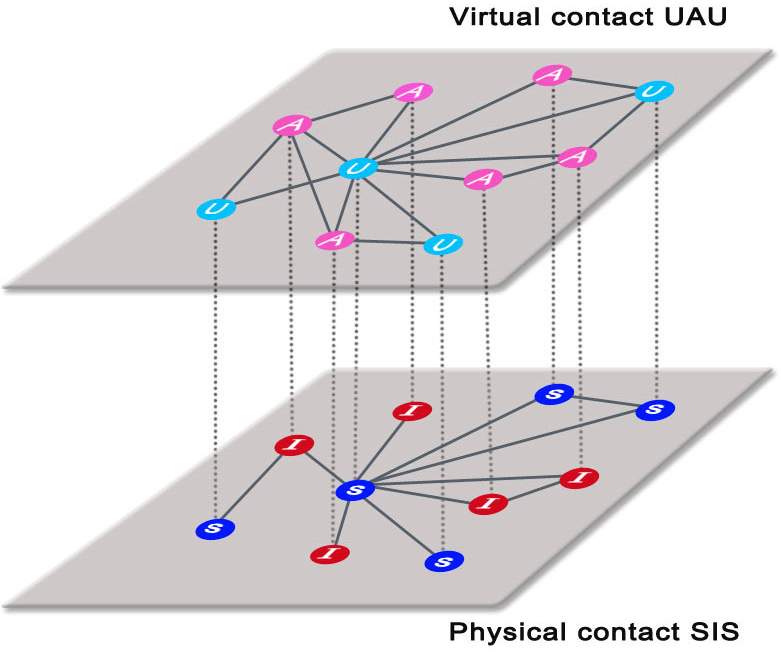
\includegraphics[width=0.6\linewidth]{0_introduction/images_introduction/multi_layer}
	\caption[Multi-layer network]{Representation of a multiplex structure. The figure is taken by the work of \cite{Granell2013} and shows the network implemented in their model. There is an awareness and an epidemic layer. In this case, the node connected with the interlayer connection represents the same individual.}
	\label{fig:multilayer}
\end{figure}

The first uses the same set of compartmental structure and mean-field models presented in the section before \ref{subsec:mean_field}. Here, from a mathematical point of view, there is no such difference in the manipulation and analysis of the system. The distinction relies on the meaning of the compartments and parameters created and on the dependence of the coefficients, which can be time and state-dependent.

The second option considers an agent-based structure. Here, considering a graph structure, composed of nodes and links between them, it is possible to classify three types of edges:
\begin{itemize}
	\item intra-layer edges, the connection of nodes on the same layer.
	\item inter-layer edges, the connection between a replica of the same node, but lying on a different layer of the structure;
	\item inter-layer edges, but coupling nodes representing distinct entities. 
\end{itemize}

 
%%%%%%%%%%%%%%%%%%%%%%%%%%%%%%%%%%%%%%%%%%%%%%%%%%%%%%%%%%%%%%%%%%%%
\chapter{Review of epidemiological behavioural and opinion models in literature}
\label{ch:literature_review}
%NUOVO TESTO
The scientific community's interest in epi-behavior models has existed for several years. Initially, as noted by \cite{Bauch_2012_overview}, the behavioral aspect of epidemiology was not given significant attention. Its development has been a gradual process, resulting from years of evolution in research.

In fact, in the initial works \cite{kermack1927}, the focus of scientists was primarily on presenting the evolution of diseases. The resulting models did not account for the effect of behavior; the population was considered homogeneously mixed, leading to random contact between susceptibles and infectives \cite{Hernandez_Vargas_2022, Mata2021}. 
It was only later, as epidemiological models proved to be effective and reliable in describing and predicting disease spread, that interest among policymakers grew. Tools capable of integrating real data with epidemiological models emerged, aiding decision-making on matters such as the duration of school closures or travel restrictions, as described in \cite{Bauch_2012_overview}.

Furthermore, new categories of models have emerged, such as agent-based models, networked models, and multi-layer/multi-system models. Despite their differing approaches, they aim to integrate various population characteristics, for example contact structure, age distribution, and movement patterns, to address the limitations of the original homogeneity assumption \cite{brauer2012mathematical}.
This focus on societal composition and behavior naturally stems from the desire to use modeling tools as a reference for decision-making in safety and health. 
One possible approach is to incorporate changes in the structure of models that describe aspects of behavior or population composition.

In these models, the behavior of the population is implicitly considered by integrating time-variable parameters that capture changes in societal behavior. This approach represents the classical modeling technique used in the formulation of epidemiological models. Examples of studies that uses this methodology for analyzing COVID-19 include \cite{Giordano_2020, Dehning_2020, Proverbio_2021}.

Although models developed in this way have proven to be powerful tools for generating insights about disease dynamics and providing recommendations to policymakers, they fall short in their ability to accurately reconstruct how populations behave during an epidemic outbreak. The desire to explore this aspect and develop a framework capable of simultaneously simulating both behavior and disease diffusion—where each mutually influences the other—has driven the development of a specific research field dedicated to behavioral epidemics.

But how can behavior be integrated into pre-existing epidemiological theory? To better address this question, we follow the classification proposed in \cite{Funk_2010}, which offers a possible subdivision of behavioral literature based on the different approaches that most articles focus on. Three major categories emerge:
\begin{itemize}
	\item The source of information used to make decisions;
	\item The type of information used to make decisions;
	\item The effect of behavioral change on the dynamic described by  the model. 
\end{itemize}

\section{Information's sources}
When analyzing the source of information, there is a clear distinction between works \cite{Vogiatzis2010} that assume governments and populations base their decisions on precise data, such as the number of infected individuals (prevalence) \cite{Collinson2014, Tyson_2020}, and those that consider more informal sources, such as conversations between people, public opinion, or media \cite{Bulai2023, Sontag2022}. These media sources include both traditional outlets like television and newspapers, as well as newer platforms like social networks.
This distinction highlights the diversity in how behavioral factors are integrated into models, reflecting the varying degrees of reliability and influence these sources have on decision-making processes during an epidemic.


Regarding information quality and the negative effect of misinformation spreading within the population, an example is the fear of vaccination \cite{Kahan_2013}. Several works analyze its effects to on the spread of infection \cite{Bauch_2012_game, Epstein_2021}.
An example of how this phenomenon can arise is the story of an article originally published by a prestigious source. Even though the thesis presented in this work was later proven wrong by the scientific community \cite{wakefield1998retracted}, the negative impact in terms of spreading fear about vaccines has persisted and, in many cases, has become deeply ingrained. In this specific case, it caused a decrease in herd immunity and a resurgence of measles \cite{Bauch_2012_overview}.

\section{Classification of different types of information}
After introducing the impact that information quality may have, another interesting aspect is related to the different types of information used in model development. Some articles focus on the effect of media on behavior \cite{Collinson2014, Misra_2011}, while others consider peer-to-peer conversations, information exchange, and beliefs among individuals \cite{Tyson_2020}. These are completely different approaches, even though they aim to achieve the same effect: simulating the evolution of people's opinions and behavior. Using media involves hypothesizing that the population is influenced by a few "central" information nodes, so the same news, data, or future predictions are shared with everyone. In contrast, models that use personal information exchanges can depict a scenario where many different ideas about the disease situation circulate simultaneously.
Another concept used in models that simulate a sort of "collective consciousness" is referred to as "awareness" \cite{Funk2009}. To model how awareness spreads in the population, it is often treated like a disease \cite{Silva2019, Granell2013, Granell_2014, Kabir_2019, Zuo_2021, Wang_2019}. Although there are many differences between these two, the main idea is that theories and concepts about a certain topic can spread among people, which can be considered at a higher level as a unified opinion. For example, there may be many different personal positions on how to respond to a health emergency like COVID-19, but it is possible to abstract the various opinions and reconstruct what the majority of people, or macro-groups, ultimately feel. They may either be more cooperative and in favor of following guidelines issued by authorities, or more focused on their well-being and inclined to act independently.
This process can be related to opinion formation studies, which aim to understand how people build their ideas \cite{Devia_2023, Devia2022} and also analyze the possible formation of opinion distributions, such as perfect consensus, consensus, polarization, clustering, or dissension.

\section{How integrate behavior in epidemiology}
While the type and source of information are crucial for understanding the basic framework and synthesizing key concepts of models that consider population behavior, the final criterion used to categorize works related to epidemiological behavior is how the influence of people's behavior on the model is integrated. This aspect is one of the most interesting and was a key focus of the literature reviewed for this thesis, as it plays a significant role in comparing and selecting relevant works for this research.

There are various ways to describe behavior in response to an epidemic and integrate this aspect into epidemic models \cite{Wang_2019, Bedson2021, Wang_2015_review}.

The first approach involves observing and simulating how connected individuals' states are linked to specific behaviors and how this influences the epidemic. This category includes agent-based models. Additionally, the reverse relationship, where disease spread alters individual behavior, has also been considered, as discussed in \cite{Granell_2014}.

There is also a broad class of mean-field models that explicitly consider the effects of behavior. In these cases, time-varying or state-varying parameters are used, resulting in a non-linear system of equations where the parameters are not constant but change based on information such as disease prevalence. Refer to paragraph \ref{subsec:homogeneous} for further details on this topic.

Another possibility involves modifying the structure or connections in the network used to simulate disease evolution \cite{Peng2021}. In network-based models, data extracted from social network structures \cite{Carballosa_2021} or small-world models \cite{Turker_2023} are often used to simulate connections between people more realistically.

In the following paragraphs, several articles are presented using this classification to simplify their categorization. Each article is then discussed in more detail, highlighting its original contribution.

\subsection{Models in which change the individual' state}
\label{subsec:individual_state}
\subsubsection{Multiple network simulated with Markovian process}
The first presented work is done in \cite{Granell_2014}. Here, a multiplex model is implemented with two different connectivity layers: the physical layer, in which spreads the disease, and the virtual contacts layer, where awareness diffuses. The article then uses the Microscopic Markov Chain approach to simulate the interaction resulting from the coupling of the two layers. Interestingly, they observe the existence of a metacritical point for the onset of the epidemic, which depends on awareness dynamic and topology of the virtual network. There is, in fact, a parameter related to the ability to influence through communication and it is observed that it impacts the onset of the epidemic only when it exceeds a certain threshold.
A subsequent work of the same authors \cite{Granell2013}, considers also the effect of a global communication agent. In this case, the metacritical point disappears. 
\begin{figure}[h]
	\centering
	\subfloat[][\emph{}]
	{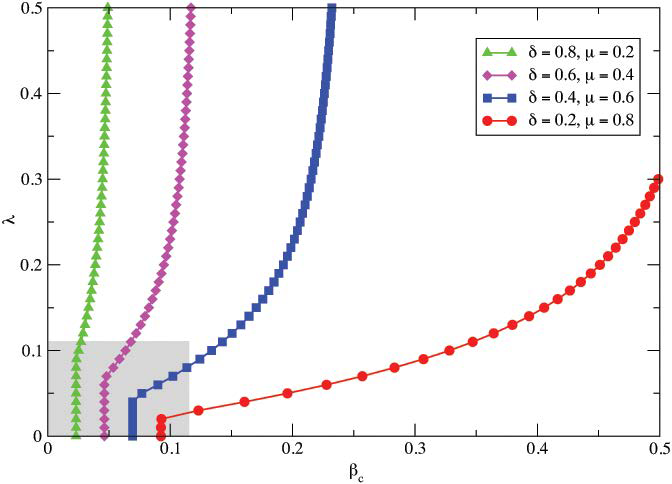
\includegraphics[width=0.47\linewidth]{0_introduction/images_review/metacritical_point_granell_2013}} \quad
	\subfloat[][\emph{}]
	{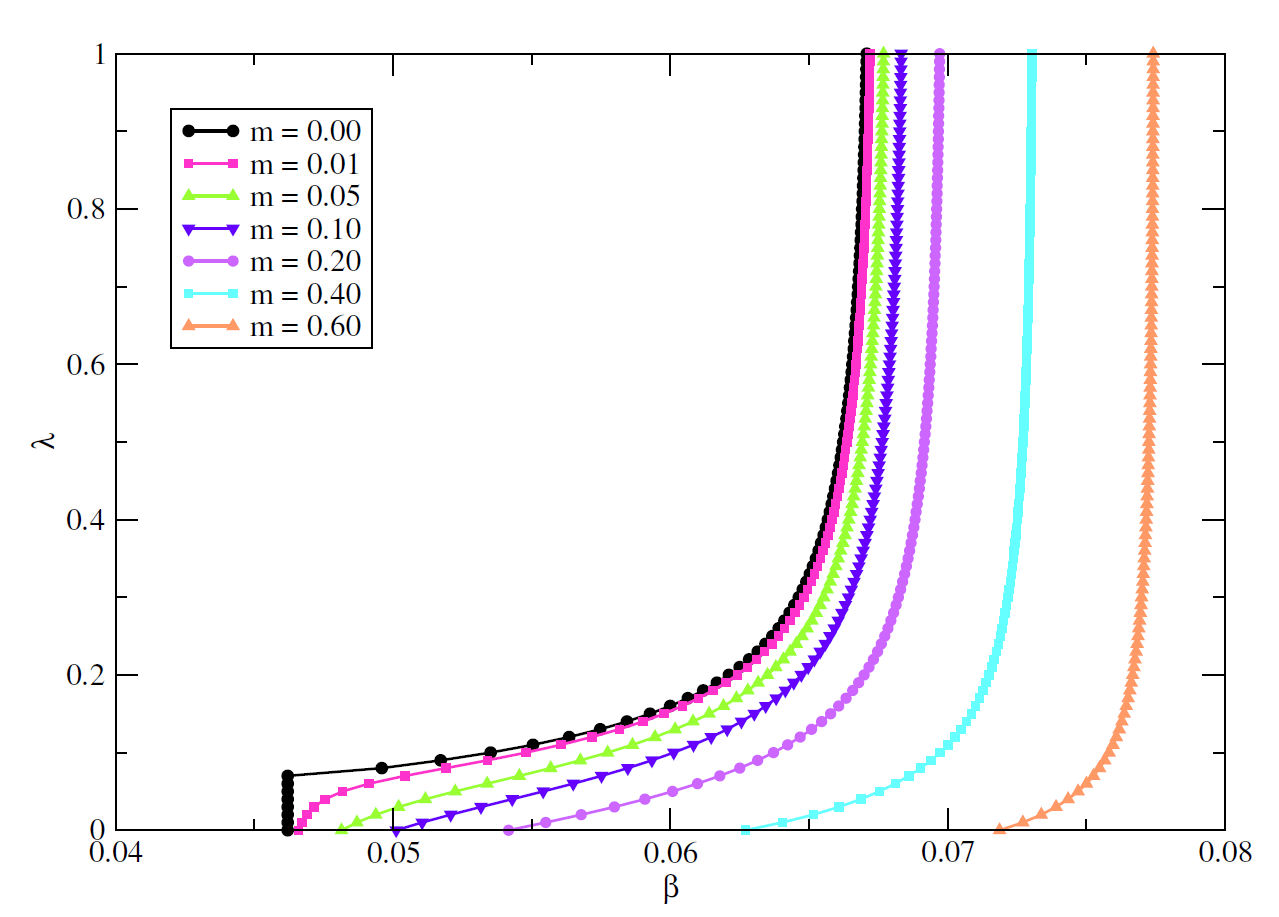
\includegraphics[width=0.49\linewidth]{0_introduction/images_review/metacritical_point_granell_2014}} \\
	\caption[Metacritical effect]{Effect of awareness communication on the onset of an epidemic. Pictures taken from \cite{Granell2013, Granell_2014}. In (a), the metacritical region is highlighted, showing that below a certain influence value $\lambda$, awareness has no significant impact on the epidemic dynamics. Conversely, in (b), the influence of a media parameter $m$, representing a global communication agent, ensures that the epidemic is always affected by the awareness layer.}
	\label{fig:sir_example2}
\end{figure}


In the article by \cite{Sahneh2013}, there is a complete description of the stochastic process at the agent level, which is useful for understanding how agent interactions are modeled across different layers using a Markovian approach. Other works using this method include \cite{Silva2019, Frieswijk_2022, Peng2021, Zuo_2021}. Except for \cite{Frieswijk_2022}, a similar double-layer structure, composed of an SIR model coupled with a UAU process, is presented in the other articles. To simulate the evolution of the complex structure resulting from the coupling of the two models, they build transition trees for all possible state changes and their respective transition probabilities. An example of both can be seen in figure \ref{fig:sir_example3}.  

\begin{figure}[h]
	\centering
	\subfloat[][\emph{}]
	{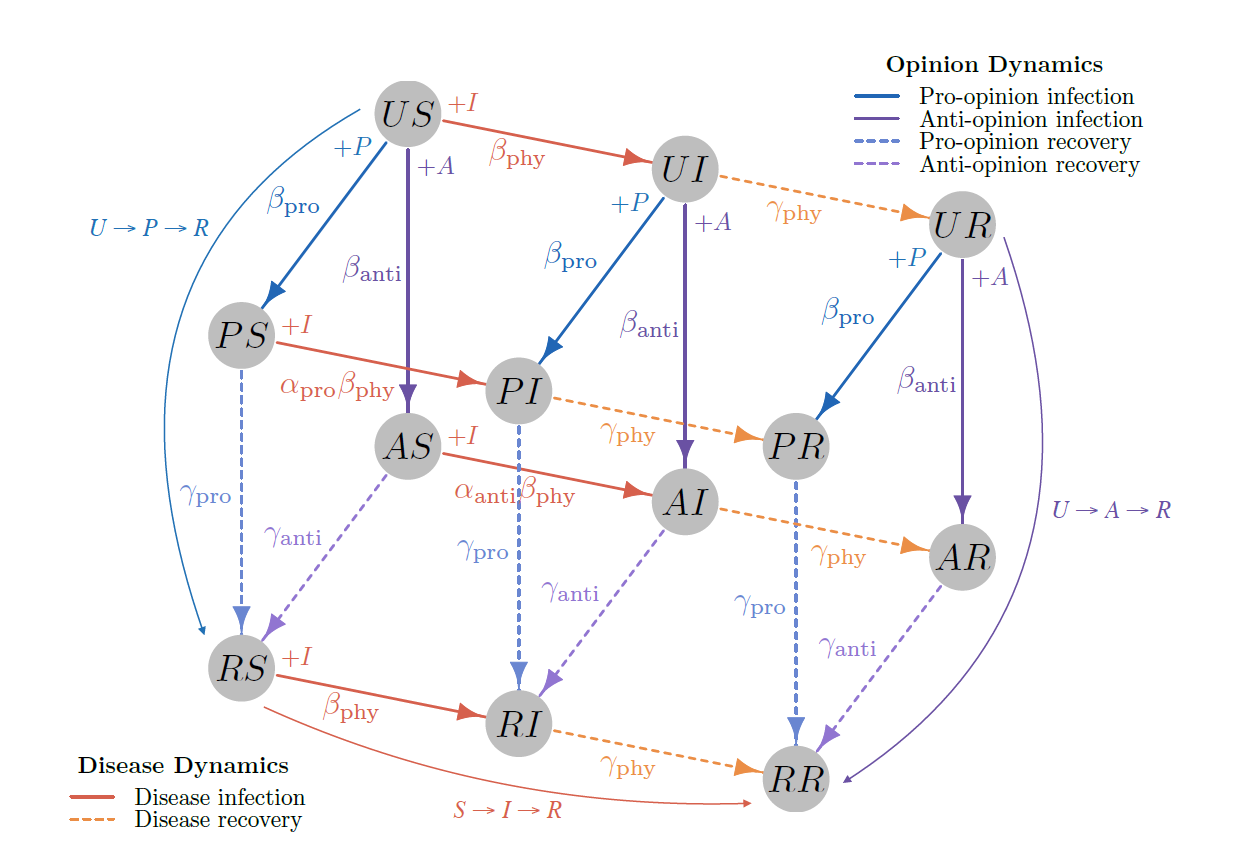
\includegraphics[width=0.63\linewidth]{0_introduction/images_review/peng_2021_bertozzi_coupled_structure}} \quad
	\subfloat[][\emph{}]
	{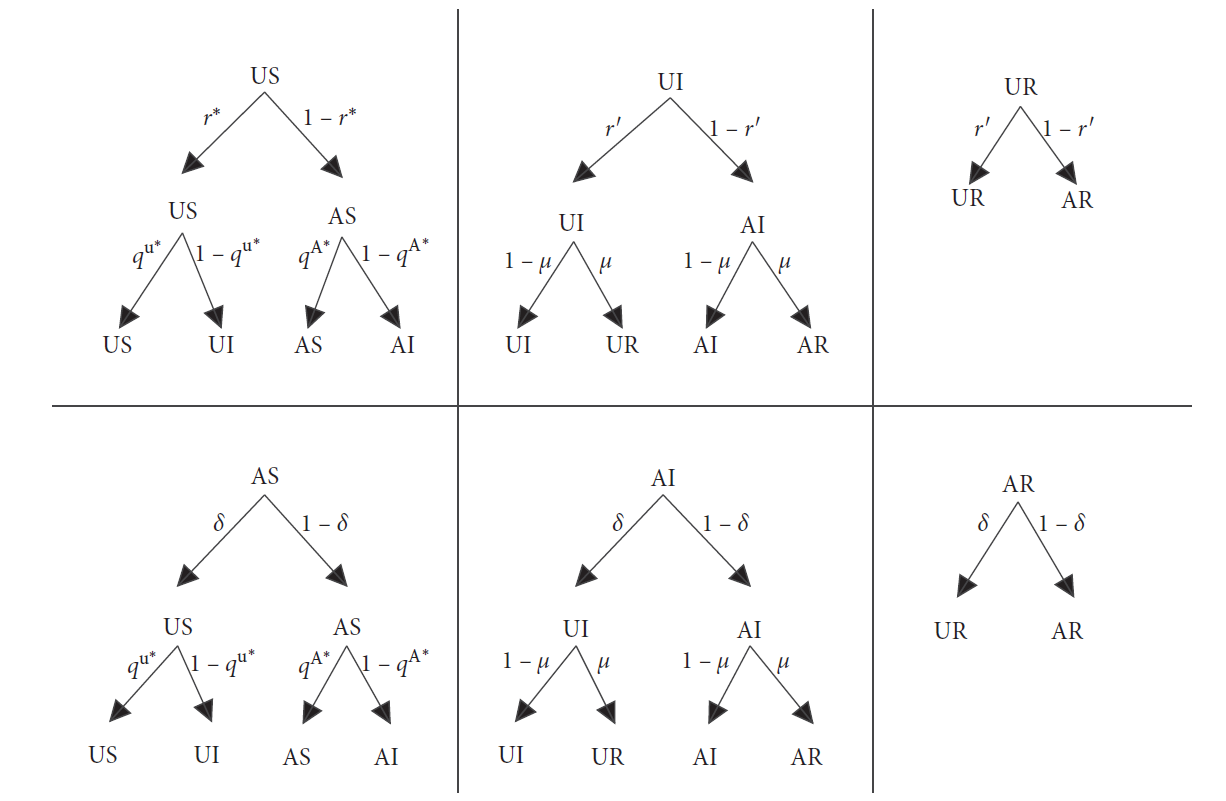
\includegraphics[width=0.6\linewidth]{0_introduction/images_review/silva2019_transition_trees}} \\
	\caption[Multiplex networks]{a) An example of a multiplex network structure resulting from the coupling of a SIR and a U-P/A-R model. b) The transition trees realized to describe the system of a SIR coupled  with a UAU model using a Markovian process. Pictures taken from articles \cite{Peng2021, Silva2019}.}
	\label{fig:sir_example3}
\end{figure}

In \cite{Peng2021}, a slightly more complex situation is described, where two possible opinions—pro-physical distancing (P) and anti-physical distancing (A)—are considered. In contrast, \cite{Frieswijk_2022} studies a simpler structure, where a SIS model is coupled with either adopting or not adopting self-protective measures.

Interesting results derived from these works include: 
\begin{itemize} 
	\item The observation of the influence of opinions on transmission speed and the final epidemic size \cite{Peng2021}. 
	\item The effect of authoritative information, publicizing epidemic prevention processes, and encouraging reasonable behavior, such as isolating when infected \cite{Zuo_2021}. 
	\item The importance of self-awareness as a mechanism to reduce disease prevalence \cite{Silva2019}. 
\end{itemize}

Finally, the experiments conducted in \cite{Frieswijk_2022} provide a stability analysis of the equilibria and explicitly calculate the epidemic threshold. Figure \ref{fig:stability_friesjiw} shows their simulations, which vary a parameter modeled as risk perception. They observe its role in the occurrence of periodic oscillations and identify a set of conditions that lead to global convergence to such a periodic solution. This is an important result, demonstrating that during an epidemic outbreak, there is a collective behavioral response, and it specifies under which conditions the situation evolves into a stable dynamic or not.

\begin{figure}[h]
	\centering
	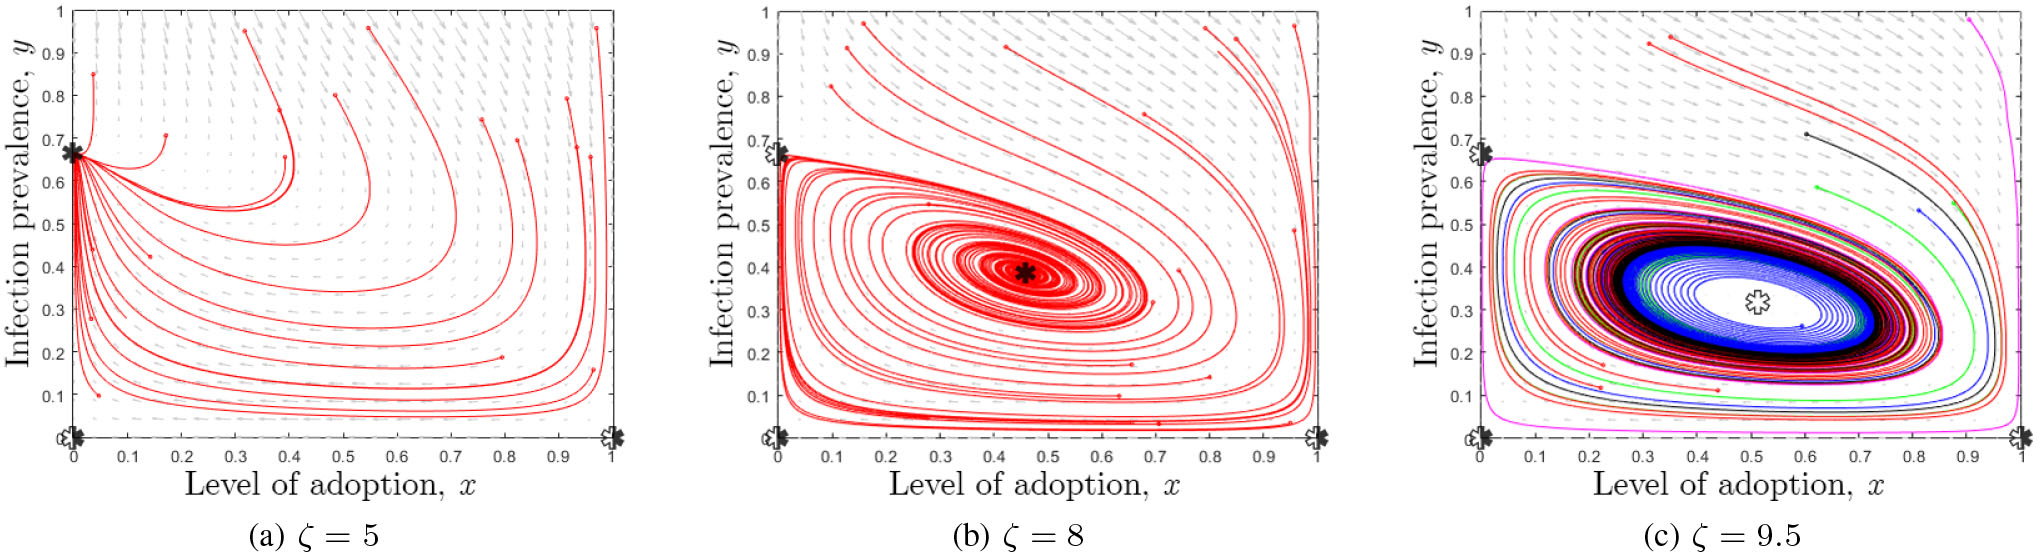
\includegraphics[width=0.95\linewidth]{0_introduction/images_review/stable_unstable_equilibria_friejs}
	\caption[Stability analysis of epi-behavior model]{Simulations taken from the article \cite{Frieswijk_2022} That show of their model evolve for different values of the risk perception parameter. Stable equilibria, saddle points and unstable equilibria are marked with a black, black-white and white asterisk, respectively.}
	\label{fig:stability_friesjiw}
\end{figure}

\subsubsection{Game theoretical models}
In the probabilistic framework, another area involves the use of game theory principles. These are used to explore strategic interactions between individuals, where participants act to maximize their utility, potentially influencing the actions of others. The concept of Nash Equilibrium is also important in this context. It is defined as "a set of strategies such that no player has an incentive to unilaterally deviate from the present strategy" \cite{Wang_2015_review}. That is, the Nash Equilibrium leads individuals to adopt strategies consistent with their goal of maximizing their benefit or utility in a perfectly rational way, forming the best responses to one another.

Many articles use this idea to model how populations adjust their behavior during an epidemic. One such example is  \cite{Auld_2003}, which focuses on the behavior of a population deciding between their sexual habits and the risk of HIV infection. The main result is derived by observing how population behavior changes as information about a possible vaccine spreads. Optimistic news lead to a decrease in the number of contacts, while pessimistic forecasts cause an increase in risky behavior, even at the same level of risk. A particularly interesting conclusion is that focusing public health messaging on dire forecasts may unintentionally lead to an increase in risky behavior.

\begin{figure}[h]
	\centering
	\subfloat[][\emph{}]
	{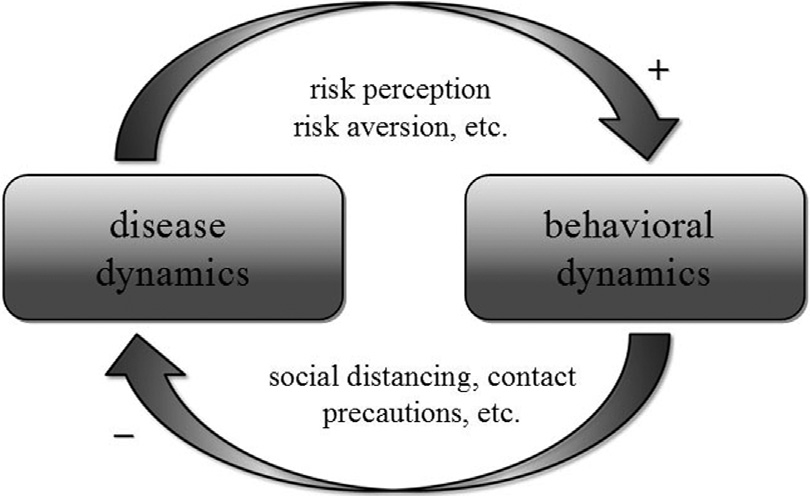
\includegraphics[width=0.38\linewidth]{0_introduction/images_review/disease_behavior_interaction_wang2015}} \quad
	\subfloat[][\emph{}]
	{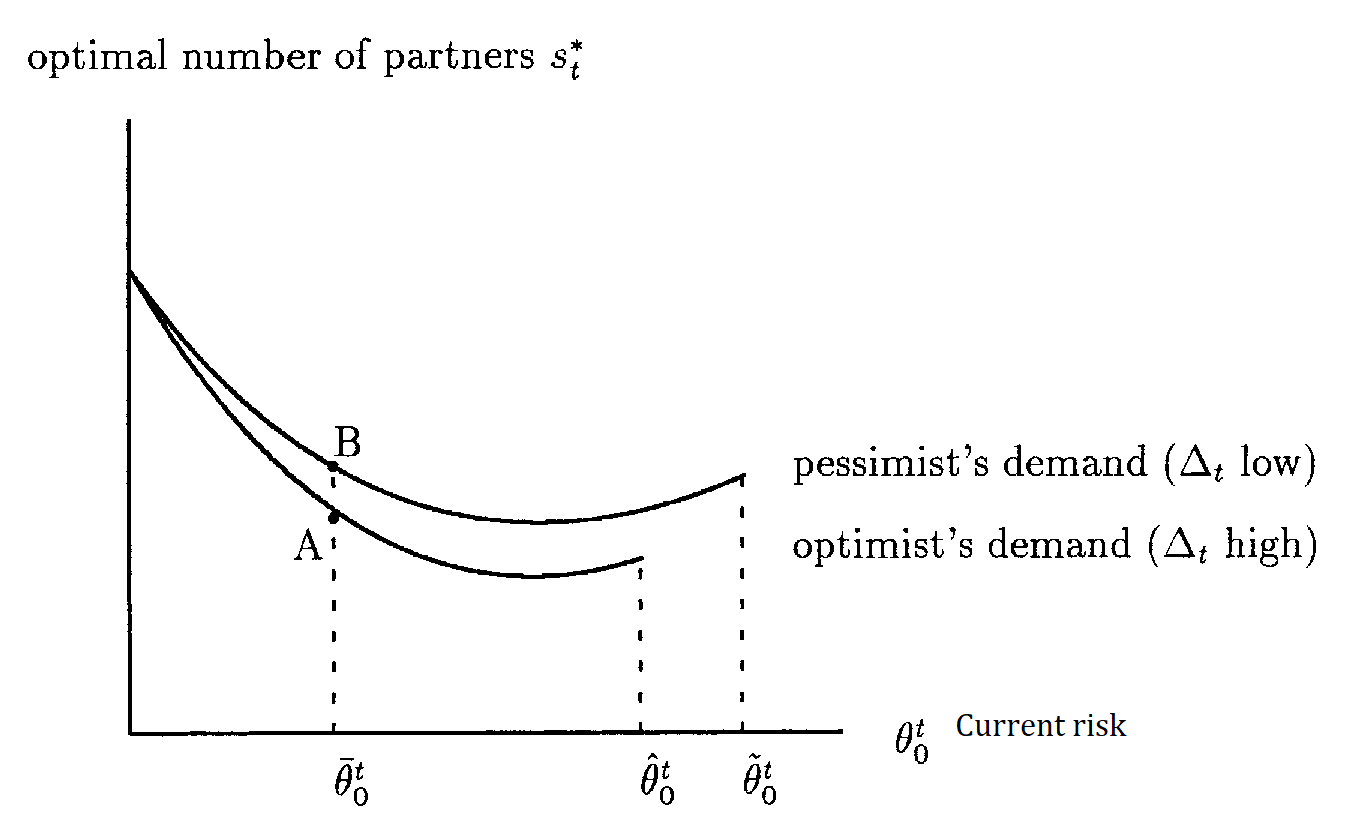
\includegraphics[width=0.58\linewidth]{0_introduction/images_review/risk_forecast_auld}} \\
	\caption[Game theory]{a) A representation of the feedback loop, taken from the article of \cite{Wang_2015}, representing the trade-off between: advantages related to avoid the disease and social cost of behave using precautions.  b) The effect on people's behavior due to optimistic or pessimistic forecasts is described in the illustration presented in \cite{Auld_2003}. The population tends to act more cautiously if there is hope that the situation will improve in the future.}
	\label{fig:abm_game}
\end{figure}

A different focus is the one that the article  \cite{Gosak_2021_game} has. Here, the behavioral change related to contact rate and especially social distancing, in the context of a pandemic situation like COVID-19  is studied to understand the efficacy of policies for partial or full voluntarily contact reduction. They aim to realize more insight into the percentage of adoption from the population of social distancing policies because increasing the quality of these estimations matters in the planning of strategies to handle a pandemic from a government point of view.

Another case study is \cite{Nunner2021}, which defines different utility functions to model the trade-off between social well-being from maintaining connections, the fatigue of doing so, and the potential physical harm those connections may cause. The main results outlined in \cite{Nunner2021} confirm that a higher number of connections between individuals leads to greater disease transmission, resulting in more infections and a shorter epidemic duration. It also highlights that "the higher the (perceived) risks of a disease, the lower the net benefit of a tie, the stronger the social distancing, and consequently the smaller the epidemic size."
Using this co-evolutionary approach, a highly correlated dynamic between the two layers emerges: a feedback loop between the spread of infection and behavioral adaptation, with structural modifications in the network occurring in the simulated scenarios.
The introduction of network-based modeling further develops this work and leads to several key findings. First, including the benefit of social connection creates multiple transmission routes for the disease. Second, a reduction in the final epidemic size only occurs when the indirect benefits are relatively low and the costs of maintaining ties are high. Finally, small changes in social behavior can have large impacts on the epidemic.
In the next paragraph, other similar studies that incorporate network models will be discussed. However, before that, a final case where the game-theoretical approach is often applied will be presented: vaccination. Many models examine the decision-making process behind vaccination, highlighting the trade-off between the benefits of getting vaccinated and the risks associated with it.
In terms of modeling, the link between behavior and epidemic spread in this case is that individuals who choose vaccination are removed from the susceptible group, with a percentage reflecting the vaccine's efficacy, thereby reducing the potential for disease transmission. In the study developed in \cite{Bauch_2012_game}, a feedback loop is established between disease prevalence and individual strategic vaccination behavior. Their model successfully fits vaccine coverage data from both the pertussis and MMR vaccine scares and can also predict future trends in disease prevalence and vaccine coverage. 
Moreover, the article highlights the phenomenon for which the vaccine fear becomes more frequent as eradication goals for more vaccine-preventable diseases are approached.

\subsubsection{Network based models}
The inclusion of networks in the modeling process has gained popularity as a tool for scientists to enhance the accuracy of their models by simulating real-world connections between people. The main goal behind developing network-based models is to create a representation of society and then use it to simulate the spread of disease. A comprehensive example of this approach is presented in \cite{VanMieghem2009}, where a method is introduced to simulate scenarios such as quarantine or regional barriers that limit population movement. By adjusting network connections—reducing contacts between nodes or cutting ties between specific regions—these models effectively demonstrate the impact of interventions like lockdowns or travel restrictions on disease transmission. They also enable analysis of how containment measures affect the trajectory of an epidemic.
Works such as \cite{Tizzoni2014} also fall into this category, utilizing urban mobility patterns as a proxy for modeling epidemics. Similarly, in \cite{Carballosa_2021}, social networks are used as a proxy for connections, hypothesizing that people's behavior in maintaining social contacts is analogous to how they might behave in the context of disease transmission.
Another innovative approach involves the development of multilayer networks, such as in \cite{Turker_2023}, where the social structure of a town is recreated. Each layer represents a different environment—ranging from homes to workplaces, distinguishing between various job types, and even considering a layer for friendships. Each individual exists across multiple layers and interacts with different groups depending on their social environment. This model found that the layer associated with friendship poses the highest risk for outbreak development, due to closer interactions and lower security measures. Consequently, even a relatively low transmissibility rate ($\beta$) can lead to a significant epidemic with many susceptible individuals involved.
\begin{figure}[h]
	\centering
	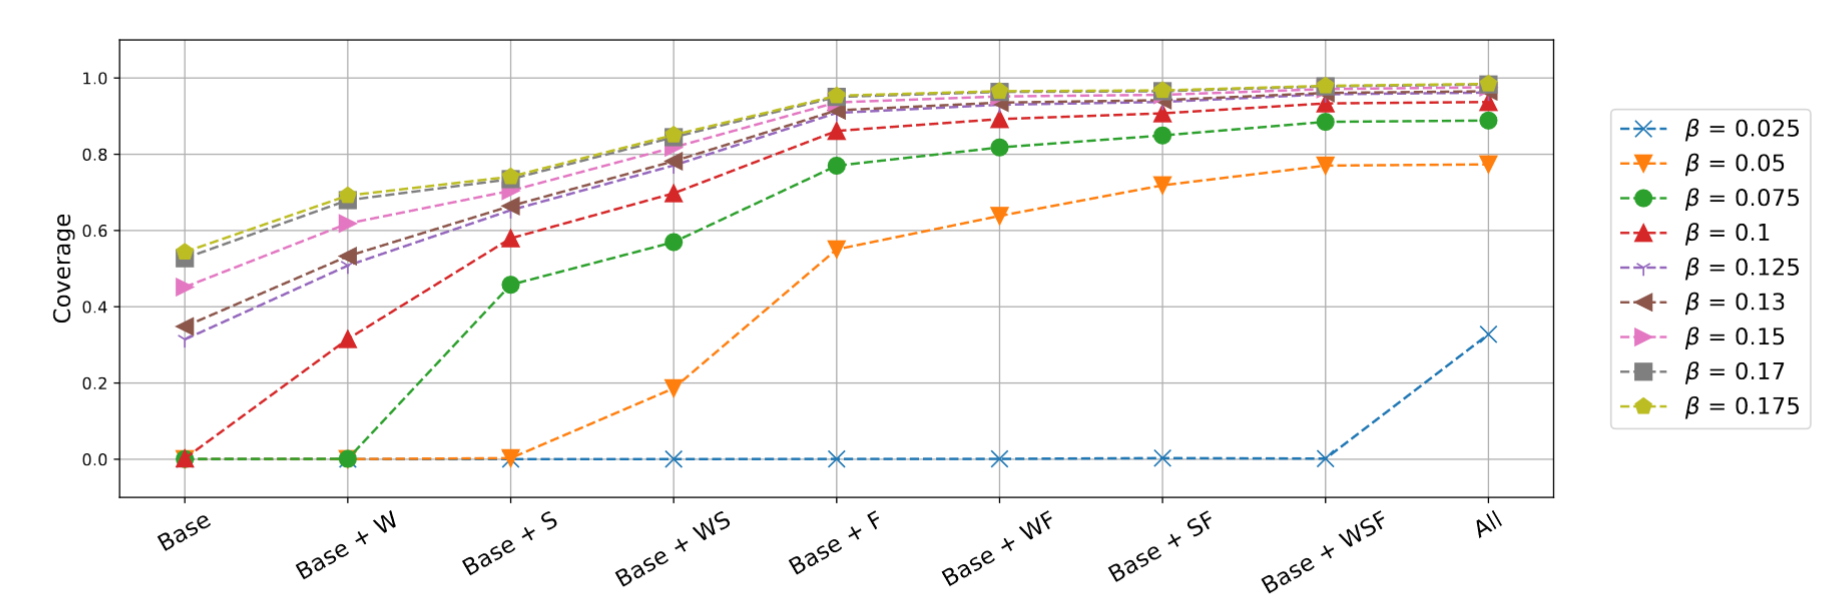
\includegraphics[width=0.9\linewidth]{0_introduction/images_review/turker_city_recreated}
	\caption[Simulation of disease spreading within a city]{In the simulation presented in \cite{Turker_2023}, a city is modeled with people divided into several social groups. They found that the layer associated with friendships is where the disease outbreak occurs with the lowest value of the infectivity parameter, $\beta$.}
	\label{fig:turkercityrecreated}
\end{figure}



\subsubsection{Threshold models}
Another possible mechanism for modeling how individuals change their actions is by observing the behaviors and opinions of their neighbors \cite{Granovetter_1978, Krassa_1988}. A well-known theoretical tool for this context is the Watts threshold model \cite{Watts_2002}, which is foundational for studying such transitions.
In \cite{Wang_2019}, various threshold models are discussed, including the Watts threshold, which is linear. In their model, each node is assigned a random threshold value based on a given distribution. The threshold represents the point at which a node changes its opinion when a certain number of its neighbors adopt a different behavior. The structure of the network is crucial for determining how opinions spread. They found that opinion propagation is most favorable in networks with low randomness and a regular structure. Additionally, they analyzed the effects of network clusters, noting that well-connected clusters can act as opinion hubs, reinforcing the spread of opinions.

\subsubsection{Ad-hoc rule-based models}
The last category of agent-based models focuses on individuals acting according to specific rules designed to simulate particular situations. A clear example of this is found in \cite{Alvarez_Zuzek_2017}, where disease propagation is modeled based on opinions for or against vaccination. The evolution of these opinions is determined by the interaction and exchange of ideas between agents and co-evolves alongside their health condition. A comprehensive set of rules is established to model all possible situations that lead to changes in both opinion and disease states. An example is visible in picture \ref{fig:alvarez_opi_vac}


\begin{figure}[h]
	\centering
	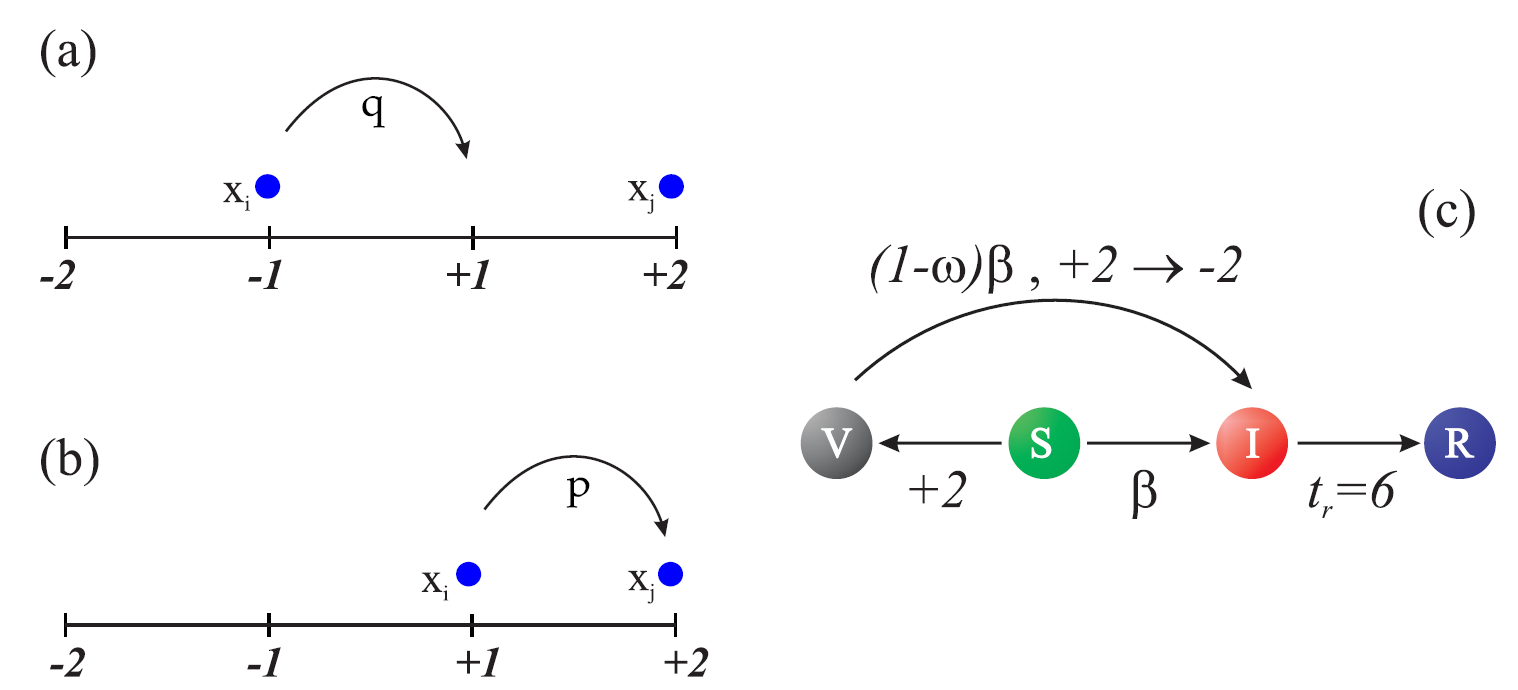
\includegraphics[width=0.8\linewidth]{0_introduction/images_review/alvarez_opi_vac}
	\caption[Rules in opinion disease model]{The picture, taken from the article \cite{Alvarez_Zuzek_2017}, illustrates the mechanisms underlying the model's dynamics. The figures on the left depict opinion dynamics: when two nodes have opposing opinions, one adjusts its state to match the other's opinion with a probability $q(a)$. If both nodes share the same opinion, the opinion is reinforced with a probability $p(b)$. The figure on the right represents contagion dynamics: a susceptible individual $S$ (green) becomes infected (red) with a probability $\beta$ and recovers (blue) after a time $t_r$. A susceptible individual can also become vaccinated $V$ (grey) upon acquiring an opinion state of $+2$. However, they can still become infected with a probability $(1-\omega) \beta$, which causes their opinion to shift to $-2$. }
	\label{fig:alvarez_opi_vac}
\end{figure}

A similar approach is developed in the article by \cite{teslya2022}, where an explicit mechanism is implemented to govern the competition between different health opinions. Individuals with a positive $+$ opinion may switch to the opposing $-$ opinion after interacting with others, following a switch rate function. By varying the parameters of this function, its behavior can become linear, saturating, or sigmoidal similar to established functions used to describe predator responses to prey population density.

Finally, the article by \cite{Collinson2014} extends the SEIR model by incorporating the effect of mass media on disease spread, using a specific set of functions. These functions account for disease prevalence, recovery rate, and media impact. The goal is to conduct a sensitivity analysis on the parameters influencing the epidemic's peak magnitude, timing, and ending. 


\subsection{Homogeneous population models}
\label{subsec:homogeneous}
This section presents the works that have most contributed to shaping the development of the thesis, the mean-field models. The assumption that the population is homogeneously mixed results in models capable of describing phenomena nationwide, which is difficult to achieve when modeling individual behavior.

However, the effectiveness of this class of models relies heavily on the modeling principles applied. Models are powerful tools, but they represent the aspects the modeler chooses to emphasize. Therefore, selecting and integrating the most promising features is crucial for creating a useful instrument. By analyzing prior works, we gain insights into what has been previously explored and the outcomes achieved.
The most interesting characteristics of various models are now presented, followed by an explanation of how they have contributed to the development of the model in this thesis.

The article \cite{Tyson_2020} was one of the first studied for its insteresting modeling approach. It integrates two dynamics: the epidemic evolution influences the parameters governing people's behavior, and, conversely, the population's behavior affects the spread of the disease. This bidirectional interaction allows for a more realistic simulation of how behavioral changes and disease dynamics influence each other.
A SIR model is associated with an opinion dynamic that occurs only within the $S$ compartment. This compartment is divided into four subgroups, representing different attitudes toward prophylactic behavior. In this way, more cautious individuals have a lower probability of becoming infected. The opinion dynamic focuses on the phenomenon of influence, modeled by a specific parameter, and on opinion amplification, a cognitive bias where confronting someone with the same belief strengthens that belief.
The most interesting aspect of their work is the concept that opinion spreads through conversation, not through a utilitarian or contagion process like fear diffusion.

A similar hypothesis of social learning is explored in the article \cite{Tanaka_2002}. In this model, both risky and cautious behaviors coexist in the population and can be transmitted. The model also incorporates the effects of clustering and the phenomenon of "cultural bias." This bias suggests that the risky trait is more likely to be adopted by cautious individuals than the reverse. Additionally, the authors introduce the concept of uncertainty regarding the infection causes, meaning that people are unsure of the best way to behave to avoid contracting the disease.


In the article \cite{Bongarti2023}, compliance with the use of NPIs (Non-Pharmaceutical Interventions) is the central focus of the behavioral component of the model. In this case, non-compliance is modeled as a social contagion: the population is divided into two groups, compliant ($c$) and non-compliant ($nc$). Using the mass-action mixing property, compliant individuals become non-compliant, but there is no recovery once their status changes. The primary goal is to understand the interplay between the stringency of lockdown measures, non-compliant behavior, and the spread of the disease.


Vaccine adoption and awareness diffusion are the main arguments developed in \cite{Zuo2022}. Awareness is present only in the Susceptible compartment, and there is a term, $M(t)$, that represents the accumulated density of awareness programs driven by various information sources. This term is influenced by several factors: awareness generated by neighboring individuals, the intensity of awareness programs in response to the prevalence of the disease, and a waning effect due to the decreasing quality or effectiveness of the information over time. Their complete model and the interplay between disease and behavior is shown in figure  \ref{fig:mean_models_1}. 
An interesting aspect of this article is that the authors evaluate their model using data from the COVID-19 vaccination campaign in China. They observe how their model effectively reproduces the population behavior and government policies during different phases of the epidemic.

\begin{figure}[h]
	\centering
	\subfloat[][\emph{}]
	{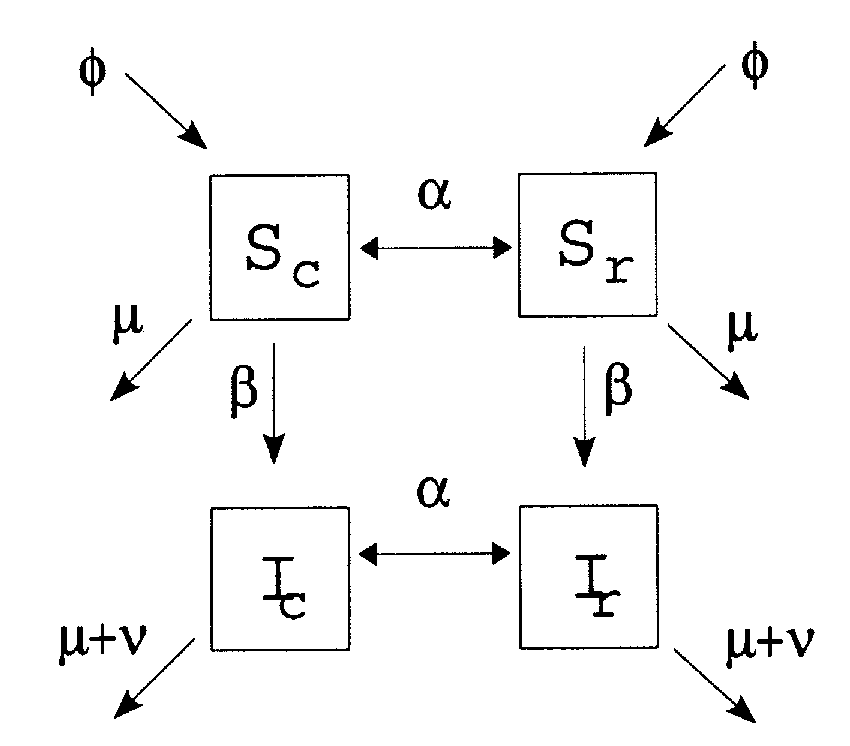
\includegraphics[width=0.35\linewidth]{0_introduction/images_review/Tanaka_model}} \quad
	\subfloat[][\emph{}]
	{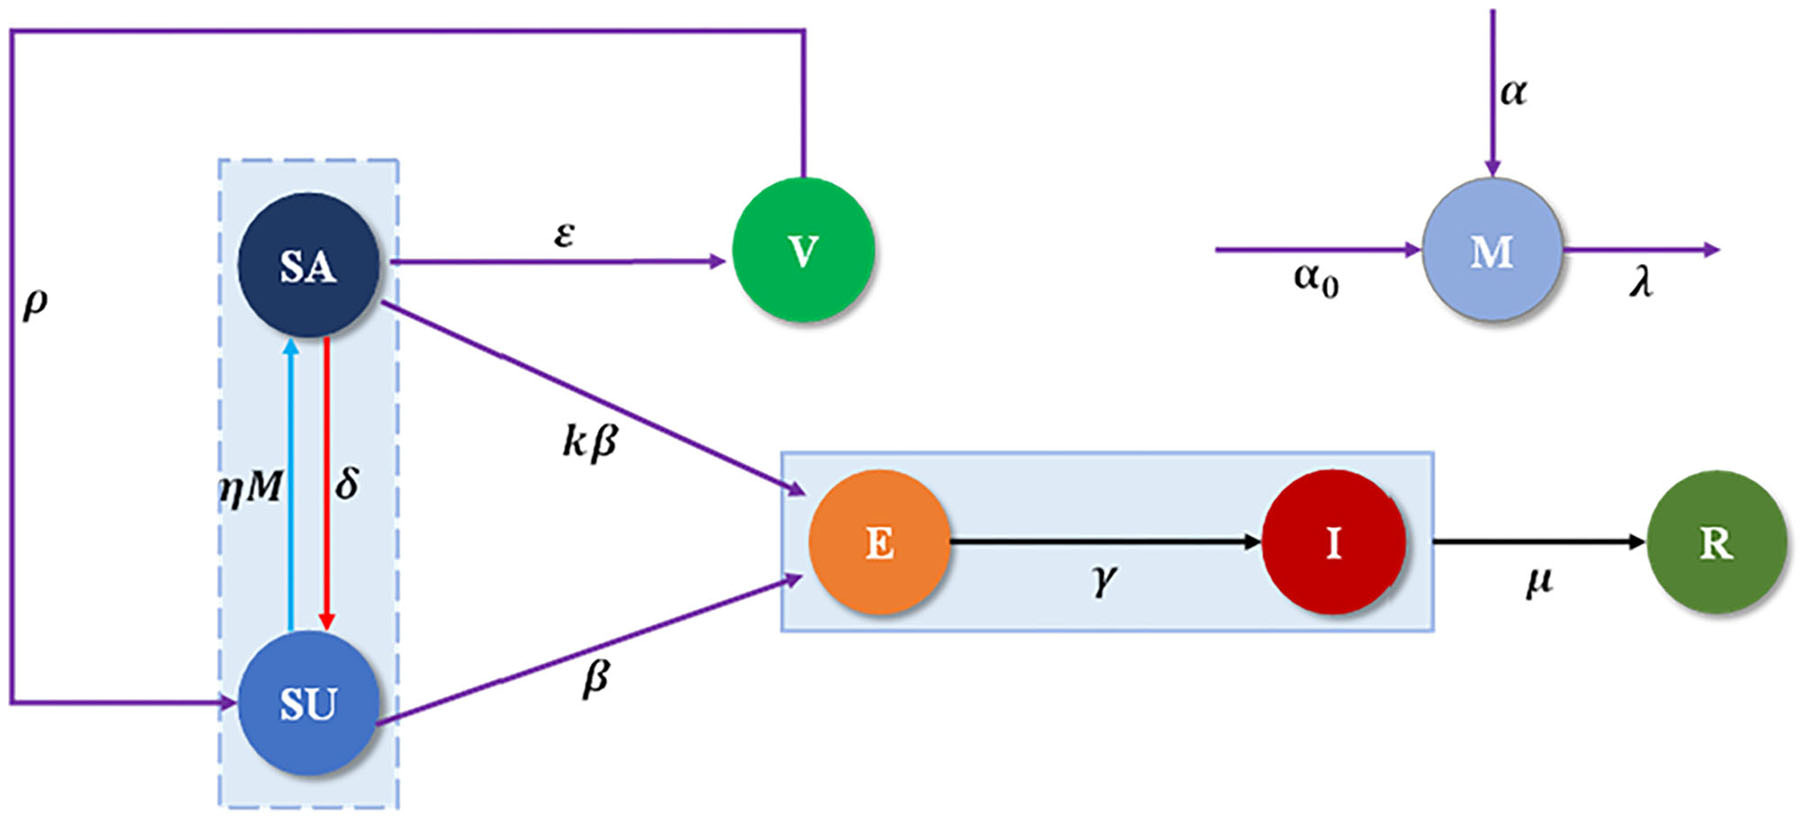
\includegraphics[width=0.6\linewidth]{0_introduction/images_review/zou_2022_SEIRVM}} \\
	\caption[Mean field models literature review]{a) The model presented in \cite{Tanaka_2002} shows horizontal layers representing behavioral diffusion, while vertical layers represent disease spread. Behavior diffuses between both infected and susceptible individuals, but this is not depicted for visual clarity. b) The model developed in \cite{Zuo2022} incorporates behavior dynamics only in the susceptible ($S$) layer, influencing both contagion rates and the probability of vaccination. The $M$ compartment follows its own dynamics, observing the state of the disease and the distribution of public opinion, and it influences the diffusion of awareness.}
	\label{fig:mean_models_1}
\end{figure}

An interesting article on the subject of behavior and vaccines is \cite{Epstein_2021}. In this model, an initially susceptible population can split into two opposing compartments, depending on what they fear more: the disease or vaccination. The model includes six compartments, with the fear dynamics occurring only in the susceptible ($S$) compartment.

In this scenario, fear of vaccination can undermine outbreak control. Initially, people may get vaccinated, but they stop too early as their fears reverse. The study also conducts a sensitivity analysis on the contact rates for the two fears, showing that transmission speed significantly affects the model’s outcomes. The results range from multiple infection waves to complete disease extinction without an outbreak, depending on the conditions.

\section{Analysis of the literature}
To conclude this chapter on the literature review, an analysis of the models discussed is presented, with a focus on how they relate to the scope and aim of this thesis. This evaluation wants to explain the key insights gained from the literature and highlight also what are the differences and novelty introduced in this work.

\subsection{Individual state models}
Referring to the models presented in the previous section \ref{subsec:individual_state}, most face the challenge of developing complex simulations to model the evolution of disease and individual behavior, but struggle to scale these simulations to the nationwide level. In many cases, small groups of agents are used, such as the 50 nodes mentioned in \cite{Nunner2021}, and even in works where a larger number of nodes is implemented, the count is typically in the thousands \cite{Granell2013}, not in the millions, as would be necessary for national-scale modeling. To overcome this difficulty, some articles use mean-field approximations, considering the limit of an infinite population size and employing statistical approaches \cite{Frieswijk_2022}.

Another critical issue these models face is the need for large amounts of data to accurately represent how populations behave during unusual situations like epidemic outbreaks. Without this data, it becomes difficult to draw precise conclusions from the models. While these models can still provide useful insights, their application for making precise, real-world predictions remains limited. They are better suited as scientific tools for exploring theoretical scenarios rather than for offering actionable advice on a larger scale. An article that demonstrates the volume of data required to test a model with real-world scenarios is \cite{Kemp_2021}. In this study, data from three different countries—Luxembourg, Austria, and Sweden—was collected, including information on total detected cases, hospitalized individuals, people in intensive care units (ICUs), and deaths. This comprehensive dataset was used to fit the model.

In the case of behavioral-epidemic models, even fewer data were available until the recent COVID-19 pandemic. As explained in \cite{Gosak2021}, this lack of data was a significant challenge. However, they show how it was partially addressed by implementing models based on population behavior with respect to influence. Despite these improvements, the availability of data today is certainly better, offering more robust insights. 

As they say: \textit{"The issue is that research has not yet provided empirical benchmarks for endogenous contact rates in disease scenarios, so it is unclear how such policies can be evaluated scientifically: ideally a policy is benchmarked against a set of counterfactuals given the disease, not compared with what was before the disease".}

\subsection{Well-mixed population models}
As stated earlier in paragraph \ref{subsec:homogeneous}, a major critique of developing complex mean-field models is that if they are not supported by consistent observation of the phenomena they aim to reproduce, their capacity to generate meaningful insights can be significantly limited. For this reason, proper empirical grounding is one of the main objectives pursued in this thesis work. The comparison of the model's emerging dynamics with real-world data is a reliable method to test the model's validity and evaluate its predictive capacity.
Reading through works in this field, a common approach emerges for modeling systems that aim to incorporate two distinct dynamics, such as behavior and disease spread. Most of these models introduce additional compartments, which represent subgroups of homogeneously mixed individuals sharing common characteristics—typically, their disease state and course of action. The primary distinction lies in how modelers handle the flow between these compartments: while some works focus on the influence of behavior solely within the Susceptible layer \cite{Epstein_2021, Tyson_2020, Zuo2022}, others implement a full double-layer model \cite{Bongarti2023, Bulai2023, Tanaka_2002}. Another key difference is whether the change in behavior dynamics is unidirectional, as in \cite{Bongarti2023}, or bidirectional, as seen in \cite{Epstein_2021, Tyson_2020, Tanaka_2002, Zuo2022}, where individuals can adjust their actions in both directions.
Notably, some of the most influential aspects drawn from the literature for this thesis include the "double fear" structure developed by \cite{Epstein_2021} and the awareness element that influences behavior change, modeled through an external node $M(t)$ in \cite{Zuo2022}. Additionally, this thesis seeks to implement a fully coupled double-layer model for behavior and epidemic spread, incorporating elements such as memory waning and fatigue, which combine with conversational mechanisms to create bidirectional flows in the behavioral model.
Unlike \cite{Tanaka_2002}, which uses a simpler epidemic model, this work employs a more complex one to accurately reflect COVID-19 data. Furthermore, the models developed in \cite{Bulai2023} and \cite{Smaldino_2021} share structural similarities with this thesis. However, \cite{Bulai2023} assumes faster information diffusion than disease transmission, decoupling the two layers, while \cite{Smaldino_2021} focuses on homophily and polarization of compartments—factors not considered here due to data limitations.
The following chapter will explain the development of the model, integrating the features and ideas here presented.


 
\chapter{Old review}

The development of a epidemiological model, that can capture the evolution of a disease influenced by the behaviour of individuals, begins from a study and review of the most significant works already present in this research topic.
These are the different main type of model that have been investigated:
\begin{itemize}
	\item deterministic/mean field models
	\item opinion models
	\item multilayer networks
	\item opinion-disease models	
\end{itemize}

Now it is presented for each of them, the main aspect and knowledge, useful for the development of my model.   

\section{Opinion models}
In the analysis performed by Wang \cite{Wang_2019}, are presented mechanism implemented to explain co-evolution spreading in complex network. The principal methodologies created over time are threshold model, that can use a linear threshold or a “Watts threshold”. Here each node has a random different threshold, based on a certain distribution. Using a threshold means that a node change opinion on the basis of its neighbours’ belief. The shape of the network is then fundamental for an opinion to spread. The best scenario is the one in which there is a low degree of randomness, and the network is regular. Also, cluster can have a reinforcement effect, if they are sufficiently connected to the resto of the graph. Their work then report analysis based on competition or cooperation of opinions “contagions”. And a SAR model is presented. Similar to a SIR, here the meaning of letter A is “adopted”. It means becoming convinced of a certain opinion, but with a probability or rate to then return to the previous behaviour. 

Also the work of \cite{Nunner2021} define and test some different models based on trade-off between the benefit of having connections and the penalty for acquiring infections. It is showed that when the behaviour of people depends on maximizing their net benefit, the individual risk perception plays an important role in the formulation of a cost function. The models derived with this so called co-evolutionary approach, have an overall dynamic very correlated between the two strati: it is a feedback loop between infection spreading, people behaviour adaptation and consequently structural modification in the network.


\section{Multilayer network}
One work based on feedback between two networks concatenated is the one performed by Peng et all, \cite{Peng2021}. Here there is explained a model based on two graphs, where one simulates the evolution of a disease, using a SIR or SIRS dynamic, and another explicit the behaviour of individual in a UPAU network. U means uninformed, P pro-physical distancing and A anti-physical distancing.  In this network the people’s conduct influence the $\beta$ coefficient of the epidemic diffusion. They demonstrate the effectiveness of having an opinion in reducing the negative effect of a disease and that lengthening the duration time for which an individual maintains opinion can help suppressing the transmission.
Study the effect of competition in a multilayer network is the objective of Teslya et all research \cite{teslya2022}. At cause of interpersonal communication individual can change their opinion. They are divided in two main groups, positive or negative w.r.t health conduct. Here is also inserted an influence due to assortatively when contacting with others. Their principal results further than the fact that opinion influence disease, is realizing a model in which the two opinions can coexist at equilibrium. There can be oscillation of prevalence due to increased transmissibility of infection. In SIR model they demonstrate a reverse correlation between the rate of social contact and the peak magnitude of infectious. The causes of oscillations in the disease dynamic are a high infection rate and a pronounced difference in infection rate between individuals with different opinions. The others important factors are the high-rate opinion exchange and high sensitivity of population to prevalence. 
In the article \cite{ Alvarez_Zuzek_2017} the opinion about vaccination is taking in consideration, into a SIR+V mean field model. Conversating is the mean used by individual to modify their opinion. With a very positive opinion susceptible individuals can choose to take the vaccine. Interesting they use a r factor to describe the extremism in opinion. Varying this coefficient, they observe that the best scenario for delay the development of an epidemic is the one where the society is neutral. So, when there aren’t compromise or persuasion, but the conversation is based on “rational” arguments.  Another works analysing two competing opinion is \cite{Epstein_2021}. Here population is sensitive to both fear of vaccine and disease. These two interact and the vaccination grow rate increases only if the fear of the disease is larger than the of vaccine.  The infection curve is very influenced by the presented dynamic, and the best scenario is obviously the one in which the fear of vaccine does not exist. However, in the case where the two fears coexist there is an improvement in the number of infected, for multiple infection waves.
The work by Auld \cite{Auld_2003}, reflect an observed characteristic in society: pessimistic expectations over the future induce a more risky behaviours. This conclusion derives observing and simulation evolution correlated to the news about a vaccine. This knowledge causes a decrease in infection rate before the vaccine becomes available. Then there is a return to normal behaviour. If there are not information, pessimism cause more risky behaviour. 
In \cite{Sontag_2022} there is another SIR and opinion model, with population that is divided in trusting and distrusting. They add in the model the effect of fading and a global force, that simulates central interventions. The main interesting conclusion of their work is that strong public intervention have a similar effect to the network to the ones obtained if the population is composed of trusting and compliant individuals. However, higher percentages of distrusting cause the model to pass a phase transition where outbreaks cannot be suppressed. 
A different approach in using a multilayer network is the one realised in \cite{Turker_2023}, where the social structure of a town is re-created. Every layer describes the places populated by individuals: from house, to work, distinguishing between different type of work, and considering a level for friendship. Each person is present to more than a layer and, in each layer, relates to different agents, based on the social group’s provenience.  Using this approach, they have found that the level in which is easier for an outbreak to develop is the one associated with friendship. Here the interaction is closer with others, the security level is lower. For this reason, a lower value of transmissibility rate $\beta$ is sufficient to have an epidemic with many susceptible involved. 

\section{Opinion-disease model}
The work done by Funk and its colleagues \cite{ Funk_2010}, it is very interesting: they collect and explain systematically the behavioural reaction of population in response to a pandemic. They classify the human behaviour subject to different possible sources of information. An information can be global available or local. This reflects the way it radiates or if develops in social cluster. Another important difference is related to objectivity. Certain information is based on belief and can change with time. This typology can be influenced by the social connections of an individual or by the influence of external agents, like media. Cognitive bias also can have an impact on our opinions: amplification, confirmation, anchoring bias. They then focus on the influence of self-initiated action in the control of disease diffusion. When an individual change its behaviour, form a modelling point of view this can influence: its probability to change state (from S to I for example). The value of $\beta$ or $\gamma$. Modification in the contact network, with a self-isolation or adherence to more cautious conduct. Fear has an important role in how people face epidemic. Due to this emotion, people can decide to get vaccinated for example (or not, if they are more frightened by vaccines). Another phenomenon observed and influenced by fear is saturation. When there is many infectious people tend to decrease their number of contact and this cause a decrement in the I curve.  Another multilayer network with two opinion, 0 where individual not take precautions and 1 where the protective measures are used, is presented in \cite{Frieswijk_2022}. This model is associated to a SIS disease one. The article studies the stability of asymptotically equilibria of the system. Assuming different value of a parameter used to describe risk perception they found a set of final possible states. The most interesting is a stable asymptotical equilibrium in which there is a periodic epidemic outbreak and a consequently population behaviour response, changing behaviour to a safer.
An analysis of people choices about vaccinations is done by \cite{Bauch_2012}, they study the feedback between the positive effect due to vaccination and the fear of being vaccinated. In fact, thanks to vaccines, the disease incidence can become very low, and the perception of risk related to them can seem larger. They implemented an approach based on game theory and using social learning.
A possibility to integrate the effect of opinion in the dynamic of an epidemic, is creating different subgroups of susceptible. They are separated according to their level of opinion, and the less they belief in use of NPI, for example, the higher probability of being infectious they have. This is the approach used in \cite{Tyson_2020}. They also implemented different functions describing the influence between opinion and the possibility to become infected. 
The influence of media has also been analysed. This is interesting, because it’s a communication channel that can be used by government, and so it is an available control measure that can be implemented, to try control the behaviour of population.  For example in \cite{Collinson2014} a parameter depending on I value simulates the effect of media covering the news about the disease. Increasing the number of infectious cause, the creation of news and other media about it. These can have as effect to induce more people practice social distance for example. Study both the effect of media, see as a central node of communication joined with opinion evolution is done in \cite{Granell_2014}. Nodes co-exist into two layer, one for disease spreading and one for awareness, (unaware-aware-unaware model). In their application the awareness process without media, must reach a certain level on the transmissibility of awareness to influence the onset of epidemic. Instead, with an influence of media, greater than zero, this “metacritical” point disappears. A central broadcast, even with a small communication influence power, as a direct effect on all the network dynamic. 
\part{Behavioural Disease Model}

\chapter{Review of epidemiological behavioural and opinion models in literature}

The development of a epidemiological model, that can capture the evolution of a disease influenced by the behaviour of individuals, begins from a study and review of the most significant works already present in this research topic.
These are the different main type of model that have been investigated:
\begin{itemize}
	\item deterministic/mean field models
	\item opinion models
	\item multilayer networks
	\item opinion-disease models	
\end{itemize}

Now it is presented for each of them, the main aspect and knowledge, useful for the development of my model.   

\section{Opinion models}
In the analysis performed by Wang \cite{Wang_2019}, are presented mechanism implemented to explain co-evolution spreading in complex network. The principal methodologies created over time are threshold model, that can use a linear threshold or a “Watts threshold”. Here each node has a random different threshold, based on a certain distribution. Using a threshold means that a node change opinion on the basis of its neighbours’ belief. The shape of the network is then fundamental for an opinion to spread. The best scenario is the one in which there is a low degree of randomness, and the network is regular. Also, cluster can have a reinforcement effect, if they are sufficiently connected to the resto of the graph. Their work then report analysis based on competition or cooperation of opinions “contagions”. And a SAR model is presented. Similar to a SIR, here the meaning of letter A is “adopted”. It means becoming convinced of a certain opinion, but with a probability or rate to then return to the previous behaviour. Also the work of \cite{Nunner2021} define and test some different models based on trade-off between the benefit of having connections and the penalty for acquiring infections. It is showed that when the behaviour of people depends on maximizing their net benefit, the individual risk perception plays an important role in the formulation of a cost function. The models derived with this so called co-evolutionary approach, have an overall dynamic very correlated between the two strati: it is a feedback loop between infection spreading, people behaviour adaptation and consequently structural modification in the network.


\section{Multilayer network}
One work based on feedback between two networks concatenated is the one performed by Peng et all, \cite{Peng2021}. Here there is explained a model based on two graphs, where one simulates the evolution of a disease, using a SIR or SIRS dynamic, and another explicit the behaviour of individual in a UPAU network. U means uninformed, P pro-physical distancing and A anti-physical distancing.  In this network the people’s conduct influence the $\beta$ coefficient of the epidemic diffusion. They demonstrate the effectiveness of having an opinion in reducing the negative effect of a disease and that lengthening the duration time for which an individual maintains opinion can help suppressing the transmission.
Study the effect of competition in a multilayer network is the objective of Teslya et all research \cite{teslya2022}. At cause of interpersonal communication individual can change their opinion. They are divided in two main groups, positive or negative w.r.t health conduct. Here is also inserted an influence due to assortatively when contacting with others. Their principal results further than the fact that opinion influence disease, is realizing a model in which the two opinions can coexist at equilibrium. There can be oscillation of prevalence due to increased transmissibility of infection. In SIR model they demonstrate a reverse correlation between the rate of social contact and the peak magnitude of infectious. The causes of oscillations in the disease dynamic are a high infection rate and a pronounced difference in infection rate between individuals with different opinions. The others important factors are the high-rate opinion exchange and high sensitivity of population to prevalence. 
In the article \cite{ Alvarez_Zuzek_2017} the opinion about vaccination is taking in consideration, into a SIR+V mean field model. Conversating is the mean used by individual to modify their opinion. With a very positive opinion susceptible individuals can choose to take the vaccine. Interesting they use a r factor to describe the extremism in opinion. Varying this coefficient, they observe that the best scenario for delay the development of an epidemic is the one where the society is neutral. So, when there aren’t compromise or persuasion, but the conversation is based on “rational” arguments.  Another works analysing two competing opinion is \cite{Epstein_2021}. Here population is sensitive to both fear of vaccine and disease. These two interact and the vaccination grow rate increases only if the fear of the disease is larger than the of vaccine.  The infection curve is very influenced by the presented dynamic, and the best scenario is obviously the one in which the fear of vaccine does not exist. However, in the case where the two fears coexist there is an improvement in the number of infected, for multiple infection waves.
The work by Auld \cite{Auld_2003}, reflect an observed characteristic in society: pessimistic expectations over the future induce a more risky behaviours. This conclusion derives observing and simulation evolution correlated to the news about a vaccine. This knowledge causes a decrease in infection rate before the vaccine becomes available. Then there is a return to normal behaviour. If there are not information, pessimism cause more risky behaviour. 
In \cite{Sontag_2022} there is another SIR and opinion model, with population that is divided in trusting and distrusting. They add in the model the effect of fading and a global force, that simulates central interventions. The main interesting conclusion of their work is that strong public intervention have a similar effect to the network to the ones obtained if the population is composed of trusting and compliant individuals. However, higher percentages of distrusting cause the model to pass a phase transition where outbreaks cannot be suppressed. 
A different approach in using a multilayer network is the one realised in \cite{Turker_2023}, where the social structure of a town is re-created. Every layer describes the places populated by individuals: from house, to work, distinguishing between different type of work, and considering a level for friendship. Each person is present to more than a layer and, in each layer, relates to different agents, based on the social group’s provenience.  Using this approach, they have found that the level in which is easier for an outbreak to develop is the one associated with friendship. Here the interaction is closer with others, the security level is lower. For this reason, a lower value of transmissibility rate $\beta$ is sufficient to have an epidemic with many susceptible involved. 

\section{Opinion-disease model}
The work done by Funk and its colleagues \cite{ Funk_2010}, it is very interesting: they collect and explain systematically the behavioural reaction of population in response to a pandemic. They classify the human behaviour subject to different possible sources of information. An information can be global available or local. This reflects the way it radiates or if develops in social cluster. Another important difference is related to objectivity. Certain information is based on belief and can change with time. This typology can be influenced by the social connections of an individual or by the influence of external agents, like media. Cognitive bias also can have an impact on our opinions: amplification, confirmation, anchoring bias. They then focus on the influence of self-initiated action in the control of disease diffusion. When an individual change its behaviour, form a modelling point of view this can influence: its probability to change state (from S to I for example). The value of $\beta$ or $\gamma$. Modification in the contact network, with a self-isolation or adherence to more cautious conduct. Fear has an important role in how people face epidemic. Due to this emotion, people can decide to get vaccinated for example (or not, if they are more frightened by vaccines). Another phenomenon observed and influenced by fear is saturation. When there is many infectious people tend to decrease their number of contact and this cause a decrement in the I curve.  Another multilayer network with two opinion, 0 where individual not take precautions and 1 where the protective measures are used, is presented in \cite{Frieswijk_2022}. This model is associated to a SIS disease one. The article studies the stability of asymptotically equilibria of the system. Assuming different value of a parameter used to describe risk perception they found a set of final possible states. The most interesting is a stable asymptotical equilibrium in which there is a periodic epidemic outbreak and a consequently population behaviour response, changing behaviour to a safer.
An analysis of people choices about vaccinations is done by \cite{Bauch_2012}, they study the feedback between the positive effect due to vaccination and the fear of being vaccinated. In fact, thanks to vaccines, the disease incidence can become very low, and the perception of risk related to them can seem larger. They implemented an approach based on game theory and using social learning.
A possibility to integrate the effect of opinion in the dynamic of an epidemic, is creating different subgroups of susceptible. They are separated according to their level of opinion, and the less they belief in use of NPI, for example, the higher probability of being infectious they have. This is the approach used in \cite{Tyson_2020}. They also implemented different functions describing the influence between opinion and the possibility to become infected. 
The influence of media has also been analysed. This is interesting, because it’s a communication channel that can be used by government, and so it is an available control measure that can be implemented, to try control the behaviour of population.  For example in \cite{Collinson2014} a parameter depending on I value simulates the effect of media covering the news about the disease. Increasing the number of infectious cause, the creation of news and other media about it. These can have as effect to induce more people practice social distance for example. Study both the effect of media, see as a central node of communication joined with opinion evolution is done in \cite{Granell_2014}. Nodes co-exist into two layer, one for disease spreading and one for awareness, (unaware-aware-unaware model). In their application the awareness process without media, must reach a certain level on the transmissibility of awareness to influence the onset of epidemic. Instead, with an influence of media, greater than zero, this “metacritical” point disappears. A central broadcast, even with a small communication influence power, as a direct effect on all the network dynamic. 




\chapter{Models description and analysis}
The model developed for the thesis work is a behavioural disease multilayer system. Before present in its entirety, a discussion about its two standalone component, a SIRS and a behavioural model is presented.

\section{Epidemiological model}

\subsection{SIR model}
\label{subsec:SIR}
The first model we present is one of the simplest used to describe an epidemic. Here the population or density of individuals is divided in three groups: Susceptible, Infectious and Recovered. 
The sum of all three groups is N, the total number of people. Usually, the groups are normalized and in this way their sum is equal to 1. 

\begin{equation}
	\frac{S}{N} + \frac{I}{N} + \frac{R}{N} = 1 
\end{equation}
The symbols used to indicate the density of each group are $s$, $i$, $r$, while the capital letters are used to specify both the name of the groups or the absolute number of participants in each one. 
Usually, the assumption that N remains stable is done. This is possible considering that the epidemic time span is much lower than the life duration of a person, and so the number of death and birth is neglected. Alternatively, we can consider that the number of births, which is an input in the S compartment is roughly equal to the number of deaths, which is an output. 
The net rate at which the number of infections increase is proportional to the number of encounters between S and I individuals, expressed by $ \beta s i $, where $\beta$ is a disease transmission coefficient. The simplest and easier way to initially explain the meaning of $\beta$ is to consider that not every contact between a susceptible and an infected person can generate a contagion. The value of $\beta$ is used to describe this parameter. 
Individuals pass from the infectious state to the recovered one at a rate $\gamma$. So the infection duration last an average time of $1/\gamma$ days. 
 In this initial model the immunity acquired after recovering from the illness is lifelong. It is equivalent for the model if after being sick a person recover or die, because it considers that it will not transmit the infection any more.  This assumption can be modified and there are often disease in which after a certain period individuals become again susceptible. Another initial simplification is the one of consider the coefficient $\beta$ and $\gamma$ constant. Also there is not a network structure defined in this model, but the population is considered homogeneously mixed. 
Most frequent alternatives groups used to expand these three initial categories are: Exposed, Asymptomatic, Vaccinated, Symptomatic.These are intermediate groups, while a possible final state that can be add is the one of the "Deceased" individuals.   
Although, SIR model is quite simple it can predict a very important aspect of an epidemic, the threshold value. Because of this, two phases can be distinguished in the disease: a free-disease scenario, while the contagion is almost disappeared and a second state in which there is a large number of infected, called endemic equilibrium.

\subsubsection{Derivation of I evolution}
The number of infected on the next day is in a discrete time $\Delta t$ given by the equation:
\begin{equation}
	I(t+\Delta t) = I(t) + [\beta S(t)I(t) - \gamma I(t)]\Delta t
\end{equation}

If the value of N is large, the variables can be considered as continuous, and imposing a time interval close to zero it becomes:

\begin{equation}
	\frac{d I(t)}{dt} = \lim_{\Delta t \rightarrow  0} \frac{I(t+\Delta t)-I(t)}{\Delta t} = \beta S(t) I(t)- \gamma I(t)
\end{equation}

Observing the dynamic development,  at $time = 0$ the population is almost composed by Susceptible, so $S(0) \approx N$, and in the first steps of contagion evolution this quantity remains stable. Considering this approximation, we have
\begin{equation}
		\frac{d I(t)}{dt} = (\beta S(0)-\gamma)I(t),
\end{equation} 
which gives,

\begin{equation}
	I(t) = I(0) \exp ^{(\beta S(0)- \gamma)t}
	\label{eqn:sol_I}
\end{equation}

 and the final set of differential equations that  describe the dynamic of infection is the following:
 \begin{equation}
 	\begin{cases}
 		dS / dt = -\beta S I \\
 		dI / dt = \beta S I - \gamma I\\
 		dR / dt =  \gamma I
 	\end{cases}
 \end{equation}


From the analytic solution  of the infectious dynamic equation in \ref{eqn:sol_I}, we can see what happens at the beginning of an epidemic. Furthermore, observing the exponential sign we can deduce the disease behaviour and how the situation can evolve.
In fact if the exponential is greater than zero the number of sick grows exponentially. While, in the opposite case, infected people tend to zero. 

The value $ \beta S(0)/\gamma = 1$ is defined as epidemic threshold. This quantity, normalized, is called $R_0$ index:
\begin{equation}
	R_0 = \beta/\gamma
	\label{eqn:basic_rep_number}
\end{equation}
It measure the intensity of the contagion, or alternatively the number of secondary infections a sick person can generate. Analysing the equation of susceptibles, with this model we see that it is always decreasing. In the SIR model, if the condition to start the epidemic is met after an increasing in the number of Infected, a peak is reached. Then, the disease begins its falling phase. It is the natural behaviour of an epidemic.
This transition happens when the value of $R = \beta S(t)/\gamma$, the effective reproduction number become less of 1.

 
INSERIRE FIGURE DAL MATLAB FATTO DA TE!e dei commenti su quello. 

Other two interesting quantities to consider when a new disease appears are, the rate of increase of the infectious and the final size of remaining susceptible at the end of the epidemic. In fact, there is a large difference when a population suffering for an epidemic, if this ends rapidly because a lot of people get sick or id this number can be controlled, and the infectious curve is flatter.

\subsection{SIRS model}
\label{subsec:SIRS}
To describe the epidemic evolution a  SIRS model is implemented. It is an extension of the most famous SIR. Its main addition is the possibility for individuals to become again susceptible after a certain period of time beyond the end of the infection. The choice of a SIR-like model is done because they are well-known as capable to describe disease like the COVID-19 CITA. From an epidemiological point of view, an "Exposed" compartment will be very suitable, to describe better the evolution of the disease. In fact, in this class of infections, after the contact with an infectious there is a certain period of incubation before the development of symptoms and contagiousness. Nevertheless this compartment was not insert in the model, because it was demonstred CITA, that also a more simple SIR can be able to model correctly the disease. In this case for realise a better fit of the real data a delay in the time scale of the system can be added in the model. This delay can be considered as an extra time to ... CITA E VEDI ARTICOLO.

The possibility of become again susceptibles is added in the model, because it is considered an interesting feature in the study of a long range time scenario. 
Considering the effect of people behaviour on the evolution of a disease, it is hypothesized that two keys moment of this influence can be the initial stages and after the first peak of epidimic. 
All'inizio il sirs si comporterà come un modello sir normal, perchè non ci saranno abbbastanza tempo trascorso perchè le persone possano reinfettarsi. Però dopo le persone posso no reinfettarsi e la loro opinione e comportamento diventerà importante. da spiegare meglio

\section{Behavioural model}
The behavioural network alone is composed of three compartments.
These are Compliant, $Co$, Careless $Ca$, Against $Ag$. 
The differential equations describing the model evolution are \ref{eq:behavioural_eq}: 
\begin{equation}
	\begin{cases}
		\dot{Ca} = -k_1 Ca Co - k_2 Ca Ag + \lambda_1 Co + \lambda_2 Ag \\
		\dot{Co} = k_1 Ca Co -  \lambda_1 Co \\
		\dot{Ag} = k_2 Ca Ag -  \lambda_2 Ag\\
	\end{cases}
	\label{eq:behavioural_eq}
\end{equation}
As initial condition the hypothesis is that at the start time of the simulation most of the population is in the Careless compartment. It is considered that if a new infection developed, it is not well known and so population have little information about it. The Careless compartment is composed by people that do not know about the risk associated with becoming infected, or that have not sufficient fear of the infection to modify their normal behaviour. 
As an example of this possible initial configuration it is considered the covid-19 case in Italy. At the early stage of its development, when the disease was spreading in China it was not considered a menace for most of the population in western countries. It is seen as a disease involving a different and far state. So, when the epidemic arrives in Europe and Italy, both the population and the government did not expect it and there is an initial time delay before the countermeasures were activated and before reliable information about the evolution of the disease are available to the population. 
There are then two opposite behavioural standings: Compliant and Against.
In the Compliant set there are population worried about the disease and that want to reduce their possibilities of becoming infected. Conversely, the Against is formed by a group of individuals that have anti-scientific ideas about the disease. Here are summarised phenomena like:
\begin{itemize}
		\item vaccine denialism;
		\item misinformation diffusion;
		\item refusal about existence of the disease;
		\item lack of trust on doctors and government policies.
\end{itemize}

%The idea of having the Against compartment is born, because specially in the early phase of a new disease diffusion, there is a lack of reliable knowledge. This documented CITA event can cause the spread of wrong beliefs in the population. It has also been demonstrated CITA that the effect of false information can eradicate, if associated with fears. The most famous example is the conviction about the possibility that vaccine against rosolioa eccettera can generate autism in child. Even if the original publication describing this effect has been scientifically disproved, this idea is still today the most popular and had caused a reduction in the percentage of vaccine population, the so-called “free rider problem”. CITA
For the study of model evolution different coefficient values has been considered.  The rates studied in the models have the following meaning:
\begin{itemize}
	\item $k_1$ influence rate between Ca and Co;
	\item $k_2$ influence rate between Ca and Ag;
	\item $\lambda_1$ rate of leave compliant behaviour due to fatigue;
	\item $\lambda_2$ rate of leave against behaviour due to fatigue.
\end{itemize}

The behaviour of the model is influenced by the value of each of this parameter. For example if the compliant have strong influence, the equilibrium of the model will be composed by most of the population with Compliant behaviour and an Against groups that tend to zero. On contrary, the opposite group composition will be the result. However, if the fatigue due to being Against is less than the one related with being Compliant the final equilibrium can be favourable w.r.t the Against group, even if the rate of $k_1 \ge k_2$.
These effects can be explained looking at the equilibrium for time that goes to infinite. It is found that depends on comparison between the ratios that can be calculated with the formula: 
\begin{equation}
	R_i =\frac{ k_i }{\lambda_i}
	\label{eq:behave_rate}
\end{equation}
This expression is the reproductive ratio of each behaviour. The behaviour with the grater value has a dominant effect on the final stable value reached by the compartments.

\subsubsection{Equilibrium and stability analysis}
There are different final equilibrium value of the system depending on the values of the parameters. In particular, the four coefficients are combined, obtaining two reproduction rates $R_1,R_2$. 
First the nullclines lines are calculated and plotted. To do this, the system can be reduced to two equations assuming the mass conservation and that the following relation holds:
$N=Ca+Co+Ag$
Then the first  two equations are rewritten, rescaling also Ca,Co,Ag with N, the humans population. Using mass conservation condition the Ag term can be substituted in the first equation, resulting in a system of two equations with two unknowns. 
The nullclines lines are calculated and varying the R1 and R2 values the different scenarios are evaluated. 
\[
\begin{cases}
	\dot{Ca} = -k_1 Co Ca - k_2 (N-Co-Ca) Ca + \lambda_1 Co + \lambda_2 (N-Co-Ca)\\
	\dot{Co} = k_1 Co Ca - \lambda_1 Co
\end{cases}
\]
The equations become
\[
\begin{cases}
	\dot{x} = -k_1 y x - k_2 (1-y-x) x + \lambda_1 y + \lambda_2 (1-y-x)\\
	\dot{y} = k_1 y x - \lambda_1 y
\end{cases}
\]
The nullclines lines can be calculated imposing $\dot{x} = 0$ and $\dot{y} = 0$. Solving the system with this condition applied gives the following two equations. For the first nullcline, with $\dot{x} = 0$:

\begin{equation}
 y = \frac{x(k_2 - k_2 x + \lambda_2)  \lambda_2}{x(k_2 - k_1)+ \lambda_1- \lambda_2}
\end{equation}
and for the second with $\dot{y} = 0$
\[x = \frac{\lambda_i}{k_i} = 1/R_i
\]
The choice of the right $R_i$ to use for the second nullcline depends on the comparison between the two reproductive ration values. The larger is the one that must be used. 
Now are presented four main possibilities of the system evolution, and the stability of the found equilibria are studied.

%%%%%%%%%%%%%%%%%%
\textbf{I case:} $R_1 >1$ and $R_1> R_2$ \\
The plots of the system evolution in this case is:

\begin{figure}[h]
	\centering
	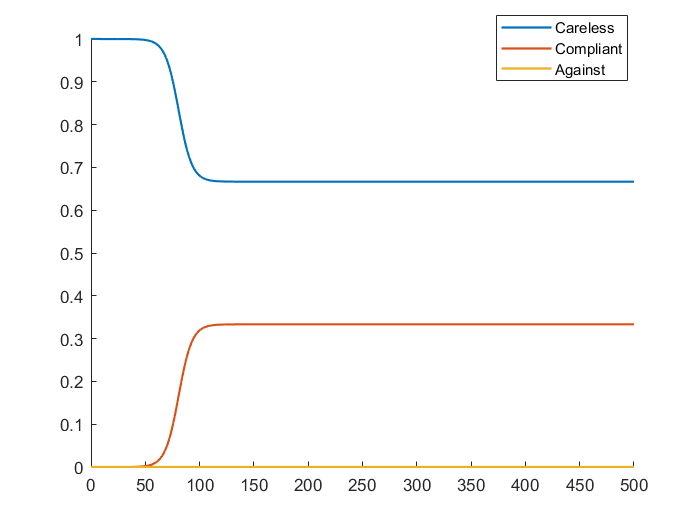
\includegraphics[width=0.7\linewidth]{1_corpo/figure/behavioural_equilibrium/r1greater1_dyn}
	\caption[Behavioural dynamic first case]{The behavioural system dynamic with $R1 > R2$ and $R1 > 1$.}
	\label{fig:r1greater1dyn}
\end{figure}
In this first scenario, as visible in figure \ref{fig:r1greater1dyn}, the Against compartment tend to zero, so the equilibrium point can be calculated as $Ca = \lambda_1/k_1$ and $Co = 1 - \lambda_1/k_1 $. 
The nullcline resulting plot is visible in \ref{fig:r1greater1nullcline}. 
\begin{figure}[h]
	\centering
	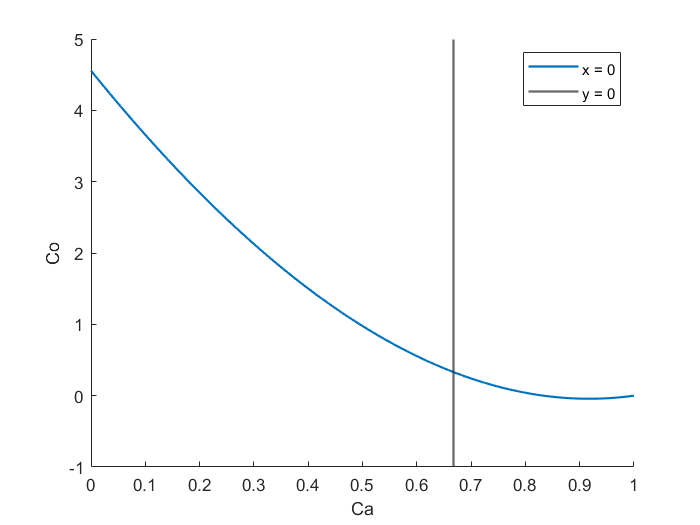
\includegraphics[width=0.7\linewidth]{1_corpo/figure/behavioural_equilibrium/r1greater1_nullcline}
	\caption[Behavioural nullcline first case]{The behavioural system nullcline lines with $R1 > R2$ and $R1 > 1$.}
	\label{fig:r1greater1nullcline}
\end{figure}

The equilibrium found as intersection of the two lines correspond to the one calculated with the numerical equation. With the Routh-Hurwitz criteria the stability of this point is verified. To evaluate if the criteria is satisfied the Jacobian matrix of the system is calculated. Then the equilibrium is used to evaluate the trace and determinant of the system in this value. To see if the equilibrium satisfies Routh-Hurwitz condition it must holds:
\begin{itemize}
	\item trace(J) $< 0$
	\item det(J) $> 0$
\end{itemize}
Both condition holds and the solution is asymptotically stable and does not depends on the initial condition.
%%%%%%%%%%%%%%%%%%

\textbf{II case:} $R_2 >1$ and $R_2> R_1$\\
The plots of the system evolution has an opposite behaviour w.r.t the first case. So here, is the Compliant compartment that tend to zero at equilibrium. 

\begin{figure}[h]
	\centering
	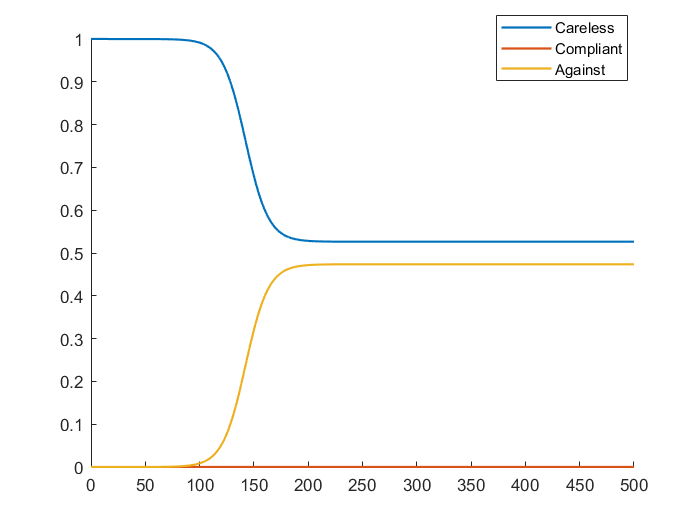
\includegraphics[width=0.7\linewidth]{1_corpo/figure/behavioural_equilibrium/r2greater1_dyn}
	\caption[Behavioural dynamic second case]{The behavioural system dynamic with $R2 > R1$ and $R2 > 1$.}
	\label{fig:r2greater1dyn}
\end{figure}
The equilibrium point can be calculated as $Ca = \lambda_2/k_2$ and $Co = 1 - \lambda_2/k_2$. 
The nullcline resulting plot is visible in \ref{fig:r2greater1nullcline}. 
\begin{figure}[h]
	\centering
	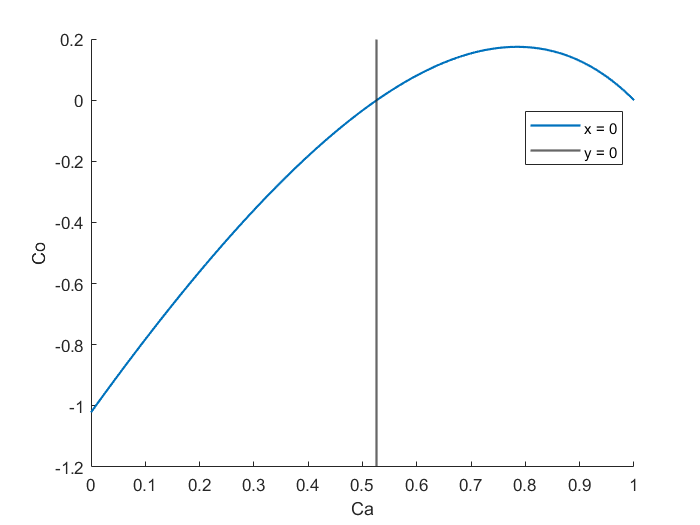
\includegraphics[width=0.7\linewidth]{1_corpo/figure/behavioural_equilibrium/r2greater1_nullcline_1}
	\caption[Behavioural nullcline second case]{The behavioural system nullcline lines with $R2 > R1$ and $R2 > 1$.}
	\label{fig:r2greater1nullcline}
\end{figure}
The equilibrium is asymptotically stable. 
%%%%%%%%%%%%%%%%%%%%%%%%%%%%

\textbf{III case:} $R_1 <1$ and $R_2<1$ \\
If both the "reproduction rates" have a value lower than one, the stable equilibrium is the one in which both Compliant and Against goes to zero. 

\begin{figure}[h]
	\centering
	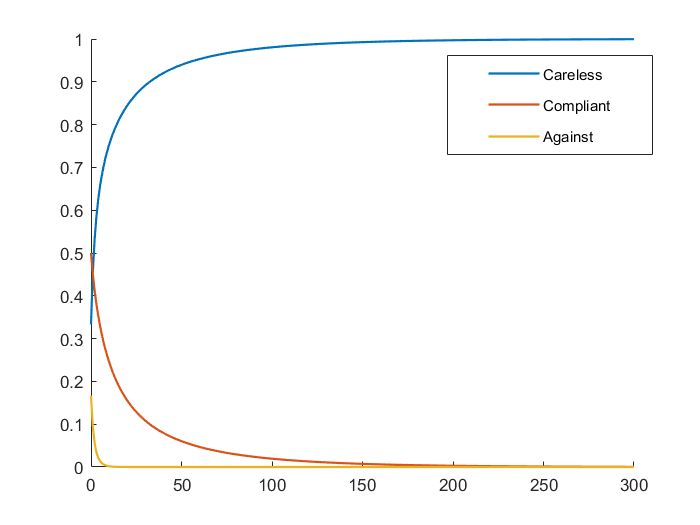
\includegraphics[width=0.7\linewidth]{1_corpo/figure/behavioural_equilibrium/r1r2less1_dyn}
	\caption[Behavioural third second case]{The behavioural system dynamic with $R1 < 1$ and $R2 < 1$.}
	\label{fig:r1r2less1dyn}
\end{figure}
From the nullcline plot \ref{fig:r1r2less1nullcline}, it can be seen that there is not an intersection. The plot of the second nullcline result in a vertical line with a value grater than one. In this condition the only equilibrium is the one for which $Ca = 1$ and both $Ag$ and $Co$ are equal to zero. 
The equilibrium is asymptotically stable. 
\begin{figure}[h]
	\centering
	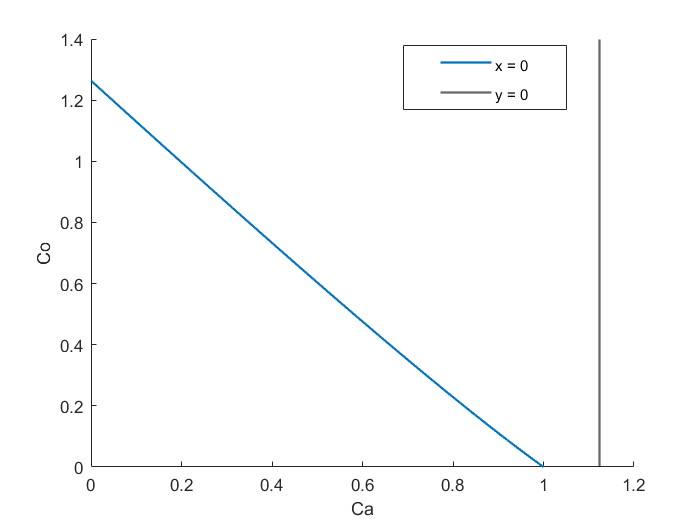
\includegraphics[width=0.7\linewidth]{1_corpo/figure/behavioural_equilibrium/r1r2less1_nullcline}
	\caption[Behavioural nullcline third case]{The behavioural system nullcline lines with $R1 < 1$ and $R2 < 1$.}
	\label{fig:r1r2less1nullcline}
\end{figure}
%%%%%%%%%%%%%%%%%%%%%%%%%%%%

\textbf{IV case:} $R_1 = R_2$ \\
This final situation is the most difficult to analyse. In fact, due to the equal value of the two influence processes, the final equilibrium of the compartments cannot be calculated using only the previous relations, but depends also on the initial condition. 
The Careless compartment can be calculated using the same equation of previous cases, and the same value is found using both $Ca = \lambda_1/k_1$ and $Ca = \lambda_2/k_2$. As it can be seen from the system evolution and nullcline plots \ref{fig:r1r2equaldyn},at the equilibrium the Against and Compliant groups are formed by a subdivision of the $1 - Ca$ part. The initial condition have an influence on how this subdivision is composed. Using the Routh-Hurwitz criterium nothing can be said on this equilibrium because the determinant of the Jacobian have a null value.
\begin{figure}[h]
	\centering
	\subfloat[][\emph{System  evolution.}]
	{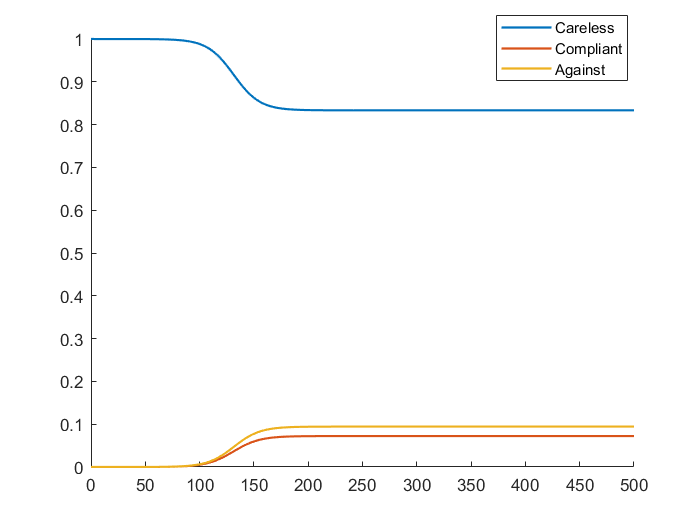
\includegraphics[width=0.47\linewidth]{1_corpo/figure/behavioural_equilibrium/r1equalr2_dyn}} \quad
	\subfloat[][\emph{Nullclines plots.}]
	{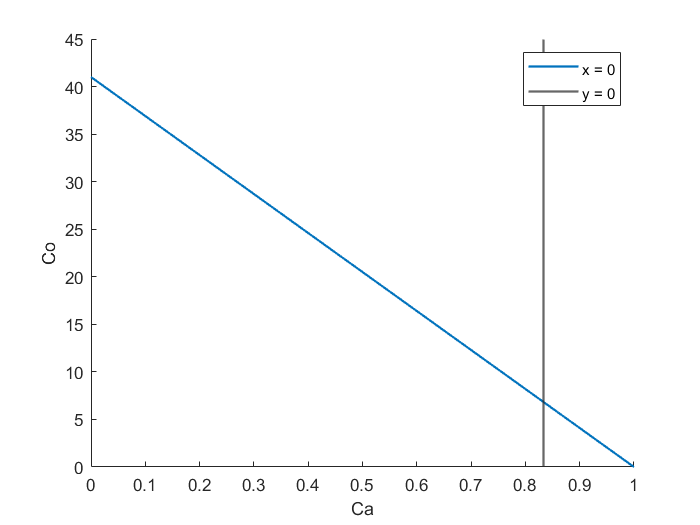
\includegraphics[width=0.47\linewidth]{1_corpo/figure/behavioural_equilibrium/r1equalr2_nullcline}} \\
	\caption[Behavioural model fourth case]{Behavioural system dynamics and nullcline in the case of   $R1 = R2$.}
	\label{fig:r1r2equaldyn}
\end{figure}

\subsubsection{Behavioural model experiment}
To better comprehend all the possible scenarios that can emerge with the behavioural model a simulation is performed. Four vectors are defined, one for each parameter of the model. A different simulation for each combination of the coefficient is then roll out. In this case the value of the parameters is kept constant during each simulation.
The range of variation of each parameter is the following:
\begin{itemize}
	\item $k_1$ between $0.1$ and $0.99$
	\item $k_2$ between $0.1$ and $0.99$
	\item $\lambda_1$ between $1/5$ and $1/30$ $d^{-1}$
	\item $k_1$ between $1/5$ and $1/30$ $d^{-1}$
\end{itemize}
We observe the evolution of the dynamics of all the states, and to present a summary of the effects we collect for each simulation data such as the final value of the compartment, the max peak value and the corresponding time in which the peak occur. 
Also here, for the sensitivity plots realization, the reproduction rates deriving from the combination of coefficients, equation \ref{eq:behave_rate}, are used. 

The first plots \ref{fig:subfig_sensitivity_behavioural} are heat maps about the final value reached by various compartments, varying $R_1$ and $R_2$.

\begin{figure}[h]
	\centering
	\subfloat[][\emph{Final Compliant compartment}]
	{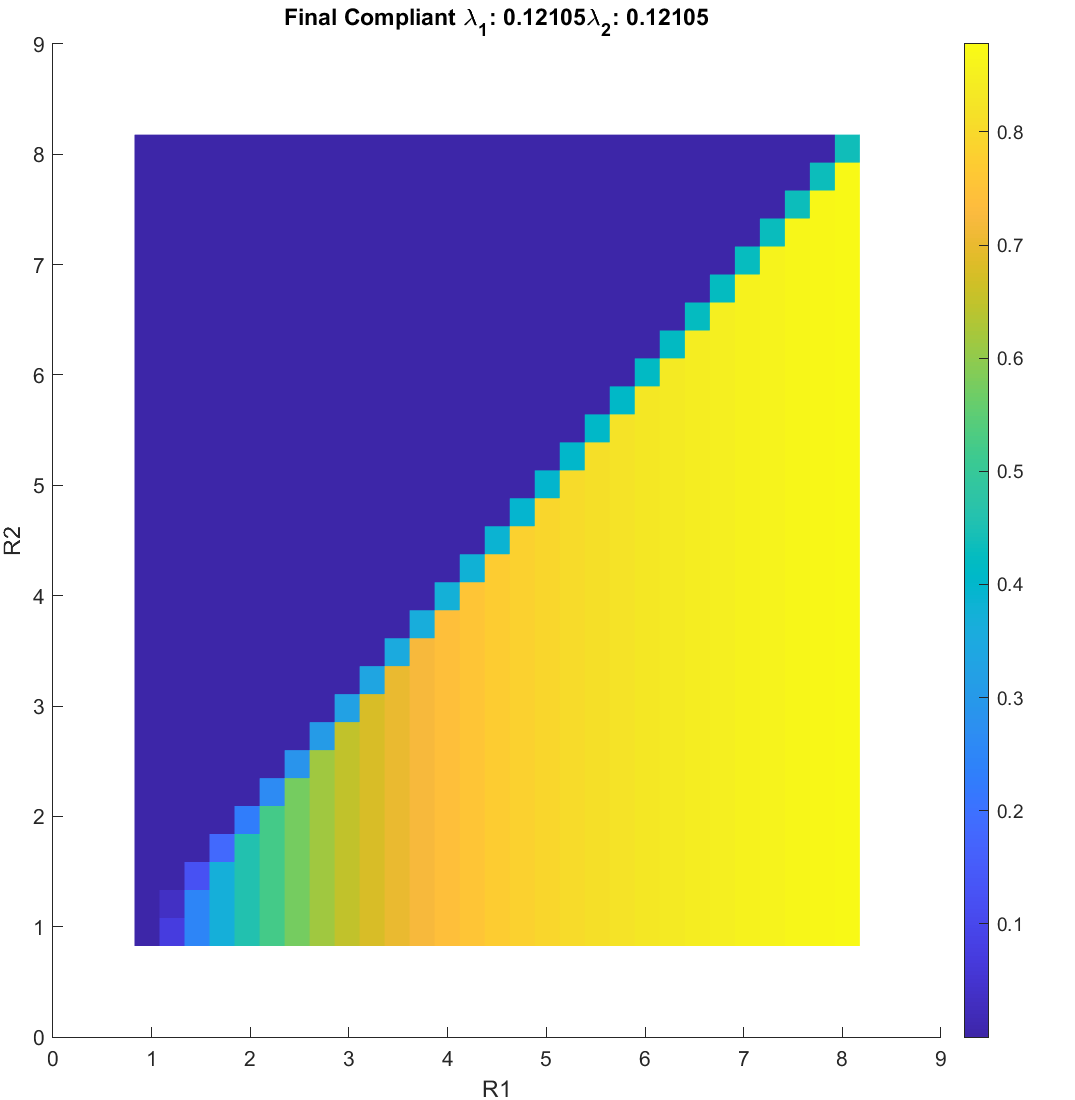
\includegraphics[width=.47\textwidth]{1_corpo/figure/behavioural_equilibrium/final_compliant_sensitivity}} \quad
	\subfloat[][\emph{Final Against compartment}]
	{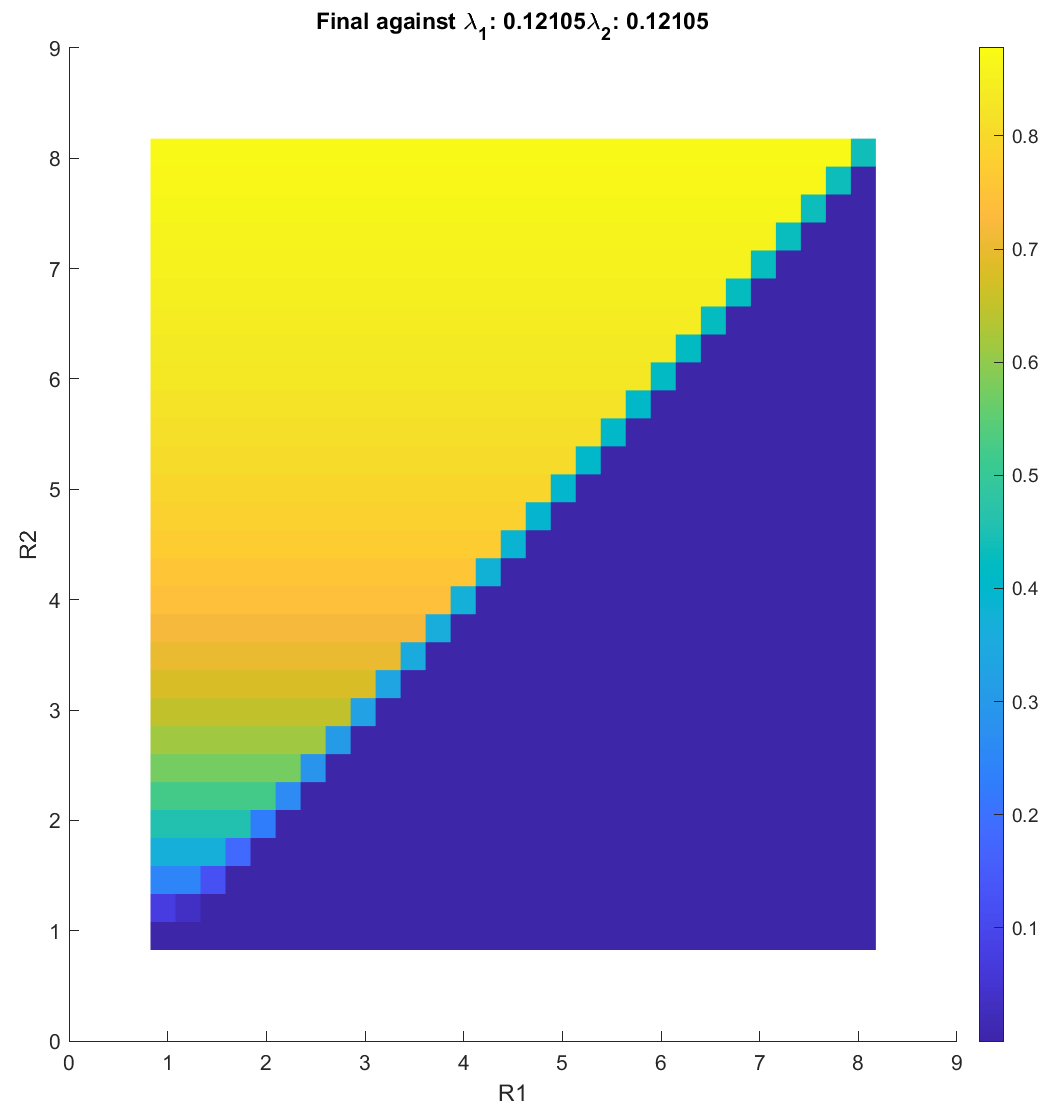
\includegraphics[width=.47\textwidth]{1_corpo/figure/behavioural_equilibrium/final_against_sensitivity}} \\
	\subfloat[][\emph{Final Careless compartment}]
	{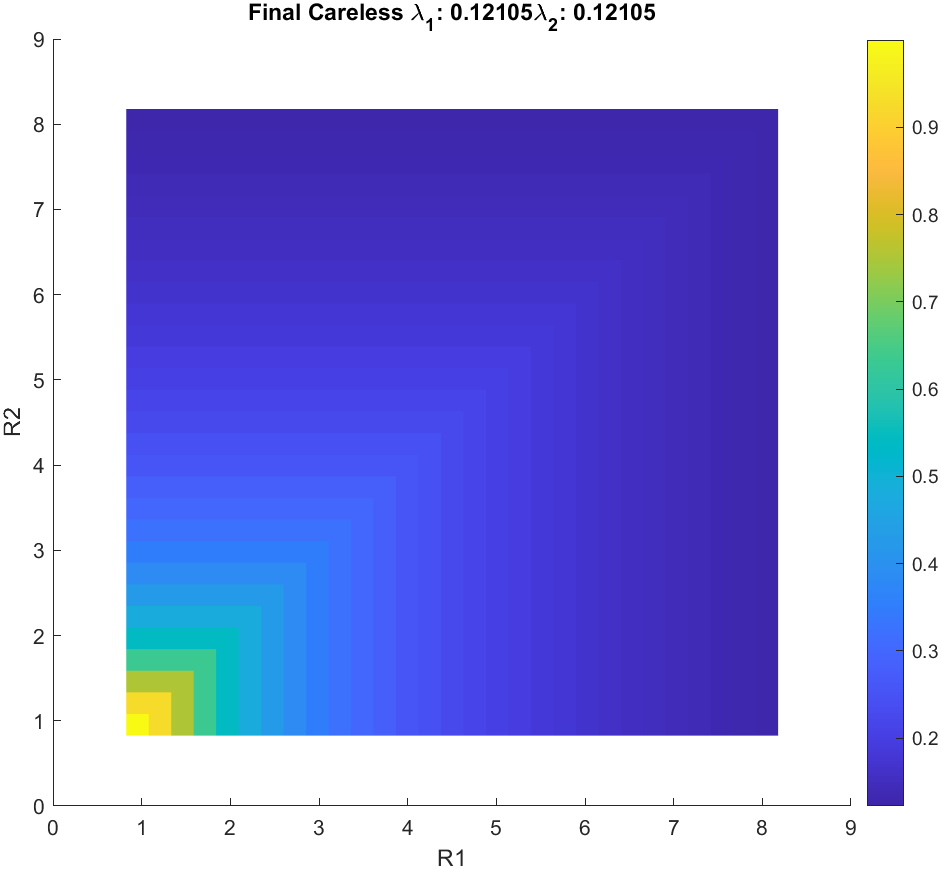
\includegraphics[width=.47\textwidth]{1_corpo/figure/behavioural_equilibrium/final_careless_sensitivity}}
	\caption[Final Behavioural compartments]{The final value reached at equilibrium by every compartment in the behavioural model.}
	\label{fig:subfig_sensitivity_behavioural}
\end{figure}

In these pictures is clearly visible the threshold effect observed in the stability analysis performed earlier. While one of the reproduction ratios becomes larger than the other, the system equilibrium is composed by the dominant group and a portion of Careless individuals.The greater is the ratio, the  smaller is the size at equilibrium of the Careless. 

Another figure in which this threshold effect can be observed is \ref{fig:subfig_sensitivity_behavioural_r1}.

\begin{figure}[h]
	\centering
	\subfloat[][\emph{Final Compliant compartment}]
	{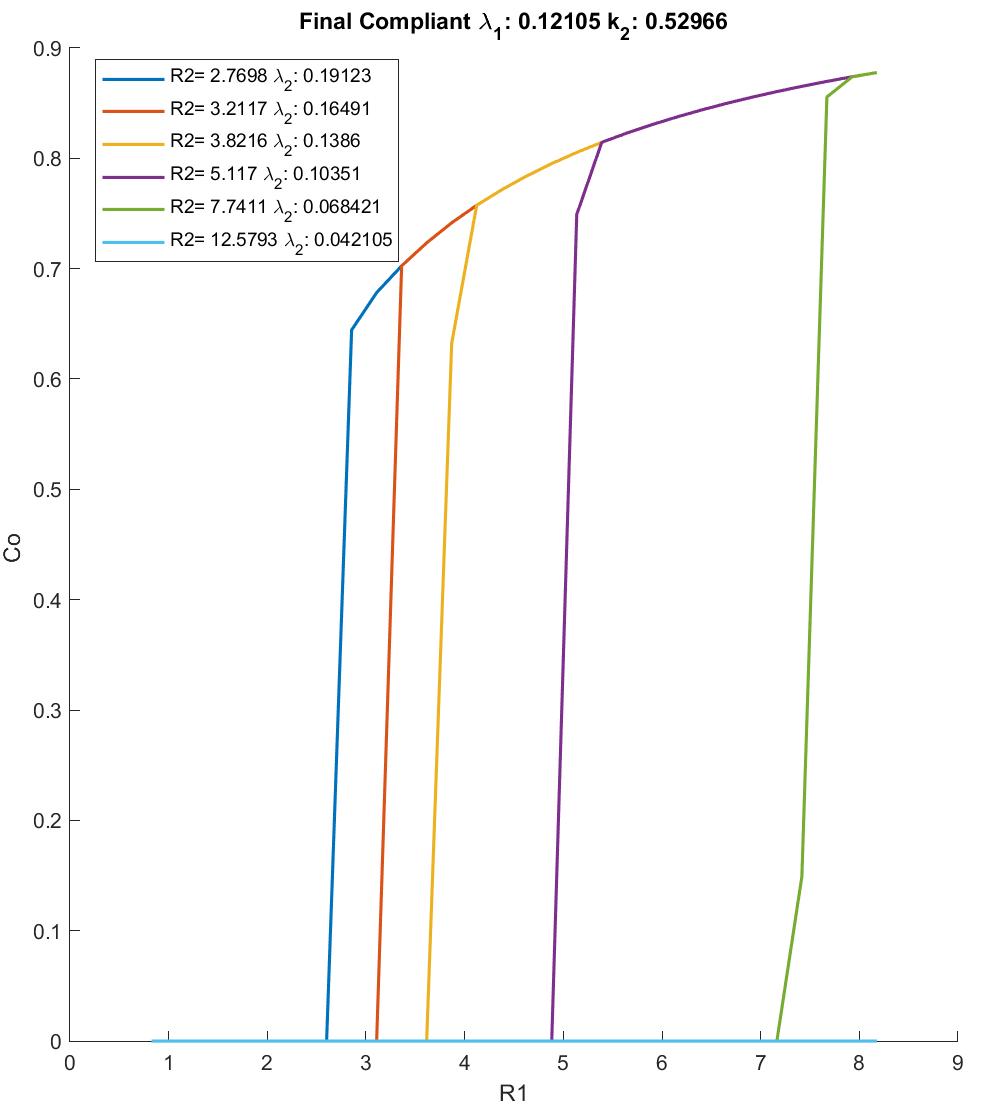
\includegraphics[height=.45\textwidth]{1_corpo/figure/behavioural_equilibrium/final_compliant_r1}} \quad
	\subfloat[][\emph{Final Against compartment}]
	{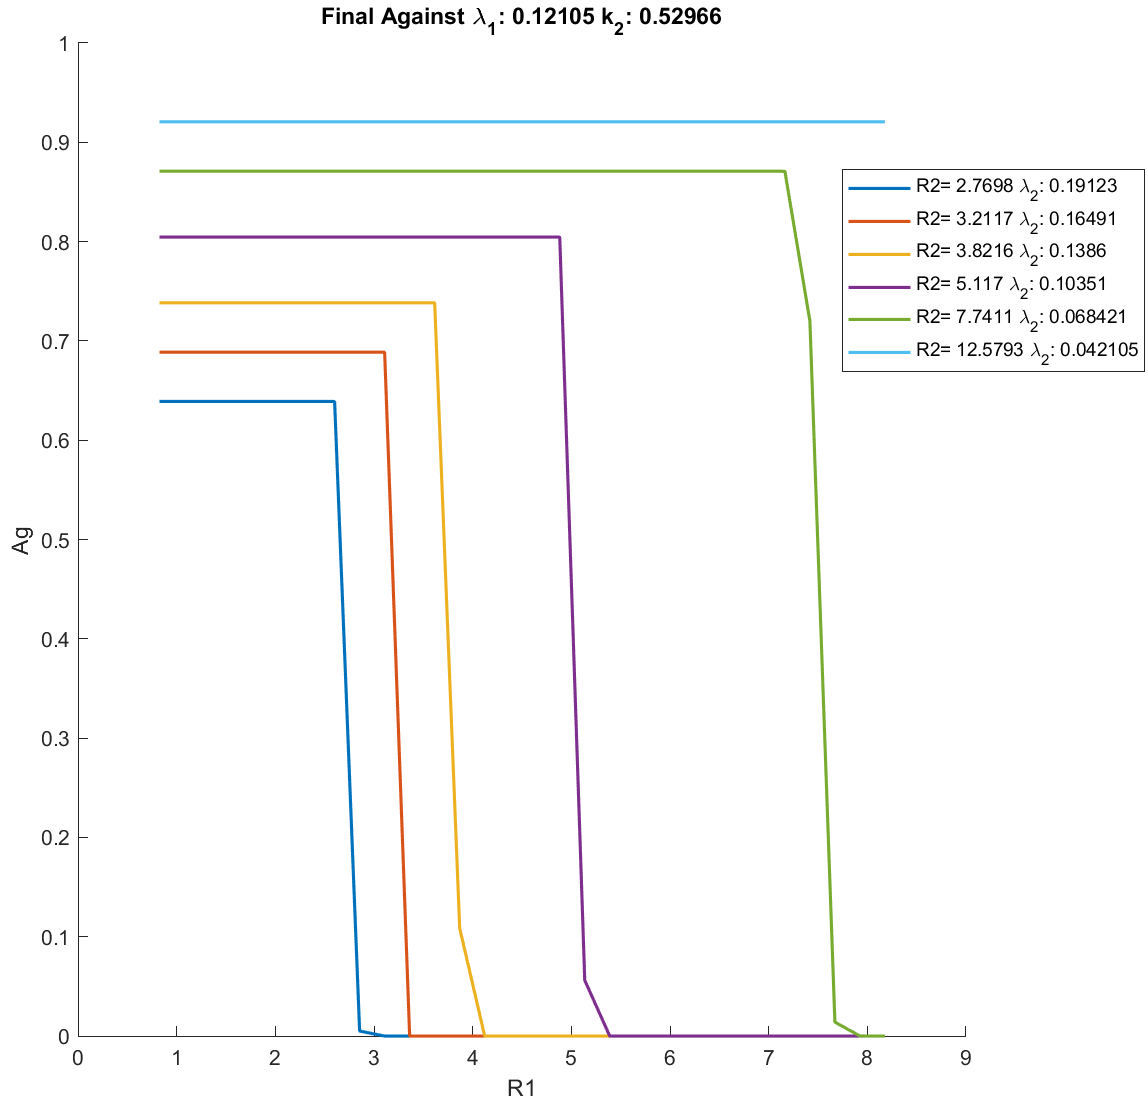
\includegraphics[height=.45\textwidth]{1_corpo/figure/behavioural_equilibrium/final_against_r1}} \\
	\subfloat[][\emph{Final Careless compartment}]
	{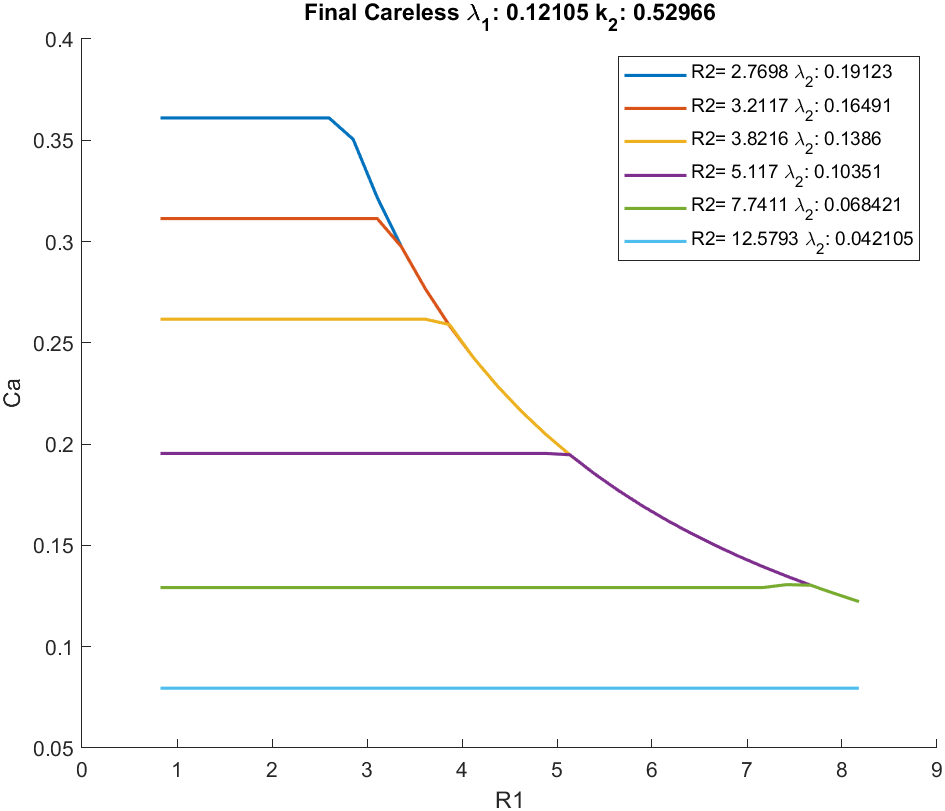
\includegraphics[height=.45\textwidth]{1_corpo/figure/behavioural_equilibrium/final_careless_r1}}
	\caption[Final Behavioural compartments varying $R_1$]{The final value reached at equilibrium by every compartment in the behavioural model varying the $R_1$ coefficient w.r.t different $R_2$ values.}
	\label{fig:subfig_sensitivity_behavioural_r1}
\end{figure}
The plots show how, for a fixed values of $\lambda_1$ and $k_2$, change the size at equilibrium of the system, varying the $k_1$ coefficient. To highlight the threshold effect due to the comparison of reproduction rates, on the x-axis is plotted the $R_1$  coefficient, that can be calculated knowing the value of  $\lambda_1$ and $k_1$. For the same reason, different $R_2$ situations are represented. 

The threshold effect is clearly visible also here. Looking at the Compliant and Against final values it can also be seen that after the $R_1$ reproductive coefficient is became dominant, the  increase is the final size observed in the Compliant plot is due to the decrease in the Careless compartment. 

Provo a scrivere, ma si va tutto molto bene
L'inglese, come disse Daniele è da sistemare, però sono su una buona strada...
%\chapter*{Acknowledgements}
\thispagestyle{empty}

Giunti alla fine della tesi, rimane solo da dedicare qualche parola a chi è stato con me durante questo intenso cammino.
Vorrei ringraziare Giulia e Daniele per tutto il sostegno, i suggerimenti e l'aiuto che hanno dedicato a me e al mio lavoro di tesi. Non è scontato essere seguiti in questo modo, grazie per tutte le cose che mi avete insegnato.

Grazie mamma e papà per tutto il supporto di questi anni e per aver saputo aspettare i miei tempi. Siete un bell'esempio per me, sia nel vostro ruolo familiare, che in quello professionale. Grazie per tutti i sacrifici che avete fatto e fate per me e Annamaria. 
Grazie nonni, il vostro amore nei confronti miei e degli altri nipoti mi riempie il cuore. Sono stato molto fortunato a poter condividere tanto fino a qui con voi e vi ringrazio per le tantissime cose fatte e tutto il tempo che avete mi avete dedicato, dal portarmi a fare allenamenti di sport vari, alle vacanze in montagna. La vostra capacità di sapervi donare agli altri, anche nel volontariato penso sia veramente qualcosa che ho imparato da voi e che porterò per sempre con me.
Grazie Annamaria, sei una super sorella, e pur con le nostre difficoltà ad esprimerci so che ci vogliamo molto bene. Aspetto sempre con molta trepidazione di vederti raggiungere i tuoi sogni e compiere i tuoi traguardi. Speriamo che le tue dermatiti ti consentano di farlo, prima di decomporti definitivamente.  


Grazie al convitto salesiano di Trento per avermi accolto e fatto conoscere alcune persone molto importanti per i miei anni universitari come Nicola, Davide, Pietro, Alessandro, Pietro, Chiara e tutti gli altri ragazzi con cui ho condiviso molto. 
Grazie Simone e Federico che durante la magistrale, compagni di progetti, mezzi flottanti, freccette e macchinine hanno condiviso molto tempo con me. Grazie a tutto il gruppetto Scout, in particolare a chi c'è praticamente sempre stato, Federico, Gabriele, Leonardo, Chimi, Andrea, Cicci e a chi è arrivato un po' dopo, Francesco e Giulio. Grazie Franz, Alberto, Mario, Michele, Leonardo, Nene, amici sia a Trento che alla fine della Valsugana, compagni di pizze doppia pasta, cinema e avventure. Penso che siate il principale bersaglio verso cui sfogo i miei interessi e il desiderio di parlarne con qualcuno. Mi spiace se vi ho tediato con videogiochi vecchi, orologi Casio, film sui sottomarini, fotografia, Doom-engine, eccetera eccetera. 

Infine grazie Marty, che mi sei stata accanto in questo non semplice percorso e hai sopportato le mie difficoltà e i miei momenti no. Ti ringrazio per tutto l'amore e il sostegno incondizionato. Da quel giorno ai mercatini sono cambiate tante cose, ma sono felice del percorso fatto e penso che con nessun altro sarebbe stato possibile trasformare anche i momenti difficili in occasione di crescita.\\

Portami \hyperref[sec:inizio]{su}, Scotty!

%%%%%%%%%%%%%%%%%%%%%%%%%%%%%%%%%%%%%%%%%%%%%%%%%%%%%%


\backmatter
%%%%%%%%%%%%%%%%%%%%%%%%%%%%%%%%%%%%%%%%%%%%%%%%%%%%%%%%%
%% 

%% BIBLIOGRAFIA

%%\cleardoublepage                    
%% per la stampa su due lati,chiude tutti gli elementi flottanti e aggiunge
%% non serve più usando biblatex

\printbibliography[heading=bibintoc]

\chapter*{Acknowledgements}
\thispagestyle{empty}

My gratitude goes to my primary supervisor Prof. Diego Giuliani who assisted me in this project, and also to my second supervisor Prof. Alessandro Giuseppe Veltri for supporting this research.

My heartfelt thanks goes to Atotus entrepreneurs, Silvia and Nicola, for helping me constantly in the first phase of the analysis and whom I consider two great human beings for their constant hard work and passion that they put in their project. I do really believe it is a unique and precious innovation in this territory. I wish them all the best.

First, I would like to thank my parents for supporting every decision and for helping me during moments of difficulties. Mum, you are such a great inspiration and your good heart is always a light in the dark. Dad, you are a great supporter with always an unstoppable humor.
I want to thank all my friends who are my greatest joy. 

I would like to thank my dearest and oldest friends Valentina and Paola with whom I have the opportunity to share a great piece of my life. Thank you for being always present and always on my side, you are my rocks.

Thank you Maria, Anna and Vale for being such an amazing sparkle and for always bringing me happiness. 

Thank you Anna, Jack and Ale, sharing these last years with you has made everything better and even the bad days were still full of beauty because of you.

At last, I would like to thank you, Riccardo, for your constant and unconditional love. I have no words to express the gratitude and the love I feel for you. 



%%%%%%%%%%%%%%%%%%%%%%%%%%%%%%%%%%%%%%%%%%%%%%%%%%%%%%%%%%%%%%%%%%%%%%%%%%%%%%%%%%%%


%%%%%%%%%%%%%%%%%%%%%%%%%%%%%%%%%%%%%%%%%%%%%%%%%%%%%%%%%%%%%

\end{document}